\documentclass[11pt]{article}
\ifdefined\pdfinfoomitdate\pdfinfoomitdate=1\fi
\ifdefined\pdftrailerid\pdftrailerid{}\fi
\ifdefined\pdfsuppressptexinfo\pdfsuppressptexinfo=15\fi
\usepackage[T1]{fontenc}
\usepackage[utf8]{inputenc}
\usepackage{lmodern}
\usepackage[margin=1.05in]{geometry}
\usepackage{amsmath,amssymb,amsthm,mathtools}
\usepackage{enumitem,booktabs,microtype}
\usepackage{tikz}
\usetikzlibrary{arrows.meta,positioning}
\PassOptionsToPackage{hyphens}{url}
\usepackage[hidelinks]{hyperref}
\usepackage[nameinlink,noabbrev,capitalise]{cleveref}
\hypersetup{pdftitle={Semialgebraic universal covers of normal projective varieties},
  pdfauthor={OpenAI}}
\setlist{topsep=4pt,itemsep=2pt}
\setlength{\emergencystretch}{2em}

\newtheorem{theorem}{Theorem}[section]
\newtheorem{proposition}[theorem]{Proposition}
\newtheorem{lemma}[theorem]{Lemma}
\newtheorem{corollary}[theorem]{Corollary}
\theoremstyle{definition}
\newtheorem{definition}[theorem]{Definition}
\newtheorem{hypothesis}[theorem]{Hypothesis}
\theoremstyle{remark}
\newtheorem{remark}[theorem]{Remark}
\newtheorem{example}[theorem]{Example}

\newcommand{\C}{\mathbb C}
\newcommand{\R}{\mathbb R}
\newcommand{\Z}{\mathbb Z}
\newcommand{\N}{\mathbb N}
\newcommand{\Q}{\mathbb Q}
\newcommand{\Pj}{\mathbb P}
\newcommand{\dd}{\mathrm d}
\DeclareMathOperator{\Aut}{Aut}
\DeclareMathOperator{\Alb}{Alb}
\DeclareMathOperator{\Pic}{Pic}
\DeclareMathOperator{\supp}{supp}
\DeclareMathOperator{\rank}{rank}
\DeclareMathOperator{\codim}{codim}
\DeclareMathOperator{\tr}{tr}
\DeclareMathOperator{\id}{id}
\DeclareMathOperator{\Hom}{Hom}

\title{Semialgebraic universal covers of normal projective varieties}
\author{OpenAI}
\date{September 24, 2026}

\begin{document}
\maketitle

\begin{abstract}
We prove the Koll\'ar--Pardon conjecture: the universal cover of a
connected normal projective complex variety is biholomorphic to a
semialgebraic open subset of a projective variety if and only if it
is a product of a bounded symmetric domain, a complex affine space,
and a simply connected normal projective variety.
\end{abstract}

\section{Introduction}\label{sec:introduction}

The universal cover of a projective variety remembers its fundamental
group through the deck action and its complex geometry through the
space on which that group acts. In complex dimension one, uniformization
leaves only the projective line, the complex line and the unit disc.
The question considered here asks whether an analogous decomposition
survives in arbitrary dimension when the universal cover admits a
finite real-algebraic description.

A subset of a complex algebraic variety is \emph{semialgebraic} if,
in algebraic affine charts, it is defined by finite Boolean combinations
of real polynomial equalities and inequalities in the real and imaginary
coordinates. We say that a complex space has a \emph{semialgebraic
projective-open presentation} if it is biholomorphic to a semialgebraic
open subset of a projective variety, with openness taken in the ordinary
complex topology. This is a condition on the complex space: the
biholomorphism is not required to be algebraic, and the deck
transformations of a covering are not required to preserve the chosen
semialgebraic structure.

A \emph{bounded symmetric domain} is a connected bounded domain in a
complex vector space for which every point is an isolated fixed point
of a holomorphic involution of the domain. We allow a point as a
zero-dimensional bounded symmetric domain. The compact factor in our
result may be singular. All universal covers and fundamental groups
below are taken in the classical topology.

\begin{theorem}[The Koll\'ar--Pardon classification]\label{thm:main}
Let \(X\) be a connected normal projective variety over \(\C\), and let
\(\widetilde X\) be its universal cover. The following conditions are
equivalent:
\begin{enumerate}[label=\textup{(\roman*)}]
\item \(\widetilde X\) is biholomorphic to a semialgebraic open subset
of a projective variety.
\item There are an integer \(m\geq0\), a bounded symmetric domain \(D\),
and a simply connected normal projective variety \(F\) such that
\[
                 \widetilde X\simeq D\times\C^m\times F.
\]
\end{enumerate}
A point is allowed as either \(D\) or \(F\). No algebraicity of the
deck transformations is assumed.
\end{theorem}

This proves Conjecture~2 of Koll\'ar and Pardon
\cite[Conjecture~2]{KollarPardon2012} in its normal-projective scope.
The three factors have different roles. The bounded factor records
hyperbolic transverse geometry, the affine factor arises from
Albanese varieties of compact fibres after finite covers, and the
remaining projective factor is simply connected. Retaining normal
singularities is essential: the assertion does not replace the
compact factor by a smooth resolution.

The group-theoretic input is the theorem of OpenAI that the entire
ordinary fundamental group of a connected smooth special compact
K\"ahler manifold is virtually abelian, meaning that it contains an
abelian subgroup of finite index
\cite[Theorem~1.1]{SpecialAbelianity}. We state its precise interface
in Section~\ref{grp:section} and apply it only to smooth compact
special manifolds furnished by Campana's core. That theorem is proved
in the separately cited companion article. The geometric construction of
the transverse quotient and the arguments passing from those compact
fundamental groups to the deck action are proved here.

\subsection{History and related results}
The affine-space case belongs to Iitaka's uniformization problem:
one asks whether a smooth projective variety covered by \(\C^n\)
is a finite unramified quotient of an abelian variety.
Nakayama proved the relevant structure theorem under semiampleness
of the canonical divisor and derived the affine-space statement
from abundance \cite[Theorem~1.4]{Nakayama1999}. This is an important
predecessor of the separation between a group-theoretic reduction
and the geometry of the Albanese map.

Claudon, H\"oring and Koll\'ar extended the question from affine
to quasi-projective universal covers. Their classification and its
general-cover extension were proved assuming smooth abundance
\cite[Theorem~1.1, Conjecture~1.2 and Corollary~1.5]{ClaudonHoeringKollar2013}.
The zero-boundary case of OpenAI's log-abundance theorem
\cite[Theorem~1.1]{OpenAILogAbundance2026} supplies exactly that
premise. Their Albanese bundle theorem itself was unconditional
\cite[Theorem~1.4]{ClaudonHoeringKollar2013}.
Semialgebraic openness admits the additional bounded symmetric
factor, and Koll\'ar and Pardon formulated the resulting product
conjecture in \cite[Conjecture~2]{KollarPardon2012}.

Koll\'ar and Pardon established a nonabelian lattice case of this
conjecture. Let \(X\) be smooth and projective, and let
\(\pi_1(X)\twoheadrightarrow\Gamma\) be a quotient such that
\(\Gamma\) acts freely, properly discontinuously and cocompactly on
an irreducible bounded symmetric domain \(D\) of dimension at least
two. Their Theorem~3 identifies a biholomorphic realization of the
associated \(\Gamma\)-cover as a semialgebraic subset of a projective
variety with a fibre-bundle structure \(X\to D/\Gamma\) and a product
presentation of that cover as \(D\times F\), with \(F\) projective
\cite[Theorem~3]{KollarPardon2012}.
Their proposed approach separates determining the fundamental group,
constructing a morphism to the locally symmetric quotient, and
proving the bundle assertion \cite[\S3]{KollarPardon2012}.
In the present proof, the intrinsic quotient is constructed before
its deck action is proved discrete and its base is identified as
symmetric.

Koll\'ar and Pardon also proved a fibre-bundle theorem that remains
an essential input here: if a morphism from a normal projective
variety to a smooth projective variety with contractible universal
cover has an entire semialgebraic projective-open pullback, then
it is a holomorphic fibre bundle
\cite[arXiv version~2, Theorem~20]{KollarPardon2012}.
Their topological and Chow-space arguments in Sections~1--2,
together with the control of invariant subvarieties in
\cite[Section~2]{ClaudonHoeringKollar2013}, are predecessors of our
compact-factor argument. We use the bundle theorem after constructing
the normal relative Albanese family, and adapt the invariant-subset
method to the polarized fibre classes on its Stein universal base.

Compactifiable K\"ahler covers give a related analytic problem.
Claudon and H\"oring, with Campana's appendix, proved an Albanese
bundle theorem after finite cover under a K\"ahler compactification
and an almost abelian group hypothesis
\cite[Theorem~1.5]{ClaudonHoering2013}. Their minimal-counterexample
analysis identifies specialness under the weaker compactification
condition \cite[Proposition~1.4]{ClaudonHoering2013}. Campana's core
\cite{Campana2004} and the compact special abelianity theorem
\cite{SpecialAbelianity} provide the group input in the present
proof. The compactification conditions in these analytic results
and semialgebraic projective openness are kept distinct.

A recent approach imposes definability on geometric data as well
as on the space. Rogov proves a metric form of the Koll\'ar--Pardon
statement for smooth aspherical projective varieties with definable
lifted K\"ahler metric \cite[Theorem~C]{Rogov2024}. That metric
hypothesis supplies information beyond a semialgebraic presentation
of the complex space. A different recent result shows that finite-CW
homotopy type alone does not suffice for the bundle conclusion:
Corr\^ea, Koll\'ar, Schreieder and Wang construct examples
with finite-CW-type universal covers whose Albanese maps are not
differentiable fibre bundles
\cite[Corollary~30]{CorreaKollarSchreiederWang2026}.
Our application of the Koll\'ar--Pardon bundle theorem retains the
entire semialgebraic pullback.

The analytic tools also have distinct roles. Real analytic
uniformization and preparation
\cite{BierstoneMilman1988,LionRolin1997} supply controlled paths and
finite scaling data. The thin-set theorem of V\^aj\^aitu
\cite{Vajaitu2000} turns small pseudoconcave omissions into analytic
holes. Bochner's tube theorem and Berndtsson's variation theorem
\cite{Noguchi2020,Berndtsson2006} identify whole quadratic fibres.
The Nadel--Frankel splitting theorem, in the form recalled by
Farb--Weinberger \cite[Theorem~1.10]{FarbWeinberger2008}, identifies
the transverse symmetric factor once the compact quotient has been
constructed. Finally, Grauert's Oka principle
\cite{Grauert1958,ForstnericPrezelj2000} turns the resulting local
compact-factor products over a contractible Stein base into a global
product. The new constructions join these inputs through projective
windows, bounded-path localization and an intrinsic quotient.


\subsection{The proof and its main obstacles}

We first explain the two geometric problems that prevent a direct
application of bounded-domain uniformization. The given cover can
contain compact positive-dimensional subvarieties, and its
semialgebraic boundary can have several successive degeneracies.
A scaling near one boundary face therefore need not produce the
whole cover or a bounded domain. Moreover, convergence on compact
subsets of a prospective limit gives only an interior inclusion:
paths in the original domains could reach other components or
escape through parts of the boundary lost under scaling. The proof
constructs the compact directions and controls this additional
boundary behaviour together.

\paragraph{Successive boundary faces.}
Write \(U=\widetilde X\). A functorial resolution of its projective
presentation gives a smooth semialgebraic open set \(V\) and a
proper modification \(\mu:V\to U\). The same deck group acts on
\(V\), with smooth projective quotient. Compact K\"ahler extension
makes \(V\) locally pseudoconvex. Near a regular real-algebraic
boundary hypersurface, the directions on which the Levi form
vanishes integrate into complex plaques. Their algebraic closures
supply projective parameter families. Scaling in the directions
transverse to a plaque produces a quadratic epigraph whose
coefficients are meromorphic functions on the plaque's projective
model. Repeating on that lower-dimensional model terminates in a
finite tower of positive-matrix inequalities. We denote this limit
domain by \(P\).

Two kinds of retention are needed in this induction. Projective
hole propagation ensures that each selected fibre is a whole
projective variety minus an analytic subset, and that these holes
stay inside a divisor defined over a full parameter box. Triangular
recentering maps control the parameters along bounded paths.
Analytic discs attached to their real orbits show that the endpoint
of every such limiting path lies in \(\overline P\).
Sections~\ref{prep:section} and~\ref{loc:section} establish these
two tools; Section~\ref{win:section} applies them to the successive
faces. The outcome includes contractibility and a bounded
realization of \(P\), together with complete real holomorphic vector
fields that span its complex tangent spaces.

\paragraph{From a window to an intrinsic quotient.}
The projective families initially describe only local regions of
\(V\). For such a region, a bounded plurisubharmonic trace of its
incident parameters is constant on every projective variety minus
analytic holes. Strict plurisubharmonicity in the parameter then
forces two intersecting fibres to coincide. Thus the fibres are
intrinsic to \(V\), even though their construction used a chosen
boundary face. Holomorphic functions that decay at the moving chart
boundaries control the exhaustion obtained by deck translations.
We call these functions \emph{guards}.
They produce a global quotient \(f:V\to M\), and a separate
compactness argument for the inverse charts proves \(M\simeq P\).
This inverse argument is what upgrades limit maps to a
biholomorphism.

The bounded realization makes \(f\) constant on the compact fibres
of \(\mu\), so it descends to \(f_X:U\to M\). To retain singular
normal compact factors, we also prepare normal fibres, flatness,
fibrewise resolutions and Whitney-stratified submersions before
choosing the scales. The exhaustive translated charts propagate
these properties to every fibre. Section~\ref{quo:section} proves
the quotient and these normal-source assertions.

\paragraph{The transverse action and its kernel.}
Put \(\Gamma=\pi_1(X)\), let \(\Lambda\) be its image in
\(\Aut(M)\), and put \(K=\ker(\Gamma\to\Lambda)\).
The induced action on \(M\) is not initially known to be discrete.
Campana's core has smooth compact special general fibres. The
abelianity theorem and a Liouville argument show that the lifts of
each such fibre have countable image in \(M\). Orbifold extension
to the full proper projective parameter families turns these
countable sets into locally finite sets. Their dense union forces
the transverse action to be discrete. After a finite cover the
action is free. The compact quotient has ample canonical bundle,
and the Nadel--Frankel splitting theorem, combined with the spanning
vector fields, identifies \(M\) as a bounded symmetric domain.
A compact-fibre monodromy map proves that \(K\) is finitely generated;
a second application of core extension and compact special
abelianity proves that it is virtually abelian.
These are the steps of Section~\ref{grp:section}; transverse
symmetry is derived within this argument.

\paragraph{Separating the affine and compact factors.}
Choose a characteristic finite-index free-abelian subgroup
\(K'\subset K\). The normal projective fibres of \(U/K'\to M\)
have fundamental group \(K'\). Their relative Albanese construction,
carried out through the simultaneous resolution and descended by
normality, gives a family of tori. The semialgebraic fibre-bundle
theorem of Koll\'ar--Pardon applies to the \emph{entire} Albanese
pullback. Its universal covering produces a proper map
\[
                  j:U\longrightarrow T\simeq M\times\C^m
\]
with simply connected normal projective fibres.

The remaining issue is variation of those compact fibres. In a
projective Chow space the fibres, and each of their polarized
isomorphism classes, form semialgebraic loci. A topological rigidity
argument forces the closure of every invariant class to be all of
\(T\). Two disjoint semialgebraic subsets cannot both be dense, so
there is only one class.
Relative Hilbert embeddings give local holomorphic products, and
the Oka principle over the contractible Stein base \(T\) gives the
global product with \(F\). Section~\ref{cmp:section} proves this
splitting and the converse. Section~\ref{sec:assembly} assembles the
classification. Section~\ref{sec:quasiprojective} records the
quasi-projective-cover consequences of smooth abundance.
Figure~\ref{fig:classification} records the three
maps constructed in the proof and the distinct group inputs.

\begin{figure}[htbp]
\centering
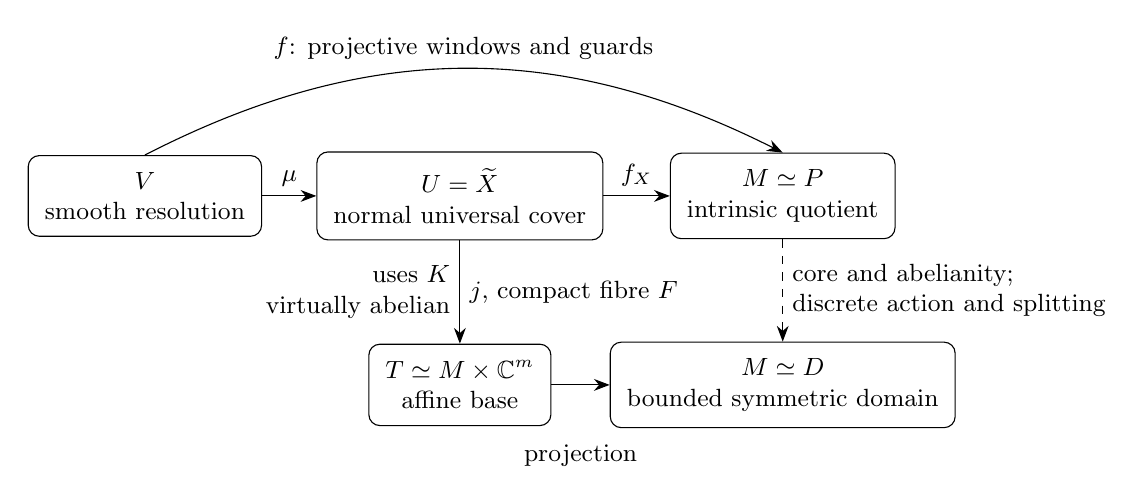
\begin{tikzpicture}[
  box/.style={draw,rounded corners,align=center,inner sep=6pt},
  every node/.style={font=\small},
  >={Stealth[length=2mm]}
]
\node[box] (v) at (0,2.4) {$V$\\smooth resolution};
\node[box] (u) at (4.0,2.4) {$U=\widetilde X$\\normal universal cover};
\node[box] (m) at (8.1,2.4) {$M\simeq P$\\intrinsic quotient};
\draw[->] (v) -- node[above] {$\mu$} (u);
\draw[->] (u) -- node[above] {$f_X$} (m);
\draw[->] (v.north) to[bend left=27] node[above] {$f$: projective windows and guards} (m.north);
\node[box] (t) at (4.0,0) {$T\simeq M\times\C^m$\\affine base};
\node[box] (d) at (8.1,0) {$M\simeq D$\\bounded symmetric domain};
\draw[->] (u) -- node[right] {$j$, compact fibre $F$}
  node[left,align=right] {uses $K$\\virtually abelian} (t);
\draw[->] (t) -- node[below=18pt] {projection} (d);
\draw[->,dashed] (m) -- node[right,align=left] {core and abelianity;\\discrete action and splitting} (d);
\end{tikzpicture}

\caption{The geometric maps in the proof. The top row constructs the
intrinsic quotient on a resolution and descends it to the normal
cover. The bottom row separates its affine and compact directions.
Solid arrows are geometric maps; the dashed arrow records the
theorem identifying the same base as symmetric. After the quotient
is constructed, compact special abelianity is used both to prove
transverse discreteness and to control the kernel \(K\) needed for \(j\).}
\label{fig:classification}
\end{figure}

\subsection{Conventions}
All projective varieties are reduced and irreducible unless stated
otherwise; a connected normal variety has one irreducible component.
A domain is connected and open. Local pseudoconvexity means local
Steinness at the boundary in the indicated ambient complex manifold.
Families with projective fibres may be analytic pullbacks of algebraic
families; bounded algebraic data in their projective variables are
specified when needed. Generic real parameters are chosen on relatively
compact boxes after removing the exceptional subanalytic sets of the
particular construction. The precise convention, including countable
families of tests, is Definition~\ref{prep:generic}.

\section{Preparation, kernels, and projective holes}
\label{prep:section}

This section supplies the two kinds of control needed for projective
windows. Preparation makes the boundary limits finite and preserves
their real parameters. The second half of the section proves that
projective fibres which are present up to algebraic holes retain this
property throughout a connected parameter domain.

All manifolds in this section are complex manifolds unless real coordinates
are specified. A locally pseudoconvex open subset of a manifold means an
open subset which is locally Stein at every boundary point. The open sets are
allowed to be disconnected before a distinguished component is selected.
Subanalytic data on a relatively compact coordinate box are always assumed
to extend as globally subanalytic data to a slightly larger box. Rational
powers of a positive scale variable are allowed. Polynomial descriptions
in projective variables are understood in a finite collection of bounded
algebraic charts, including charts at infinity. In this paper,
\emph{bounded algebraic data} means that one such finite atlas and
uniform finite bounds for the number and degrees of the polynomial
fibre equations and tests have been fixed. The coefficient arrays
depend analytically, or globally subanalytically, on the retained
parameter boxes as specified in each statement. For an algebraic
map, the same convention is imposed on its graph. A \emph{bounded-data
semialgebraic family} has a fixed finite Boolean description of this
kind in real and imaginary fibre coordinates. These are bounds on
finite algebraic complexity; estimates for coefficients, scale
matrices or their inverses are stated separately when required.

\subsection{The preparation conventions}

\begin{definition}[Generic real parameters]\label{prep:generic}
An assertion at generic parameters in an open real box means that it holds
outside a locally finite union of subanalytic subsets of smaller dimension.
When countably many fixed compact boxes or positive accuracies are tested,
a countable union of such exceptional sets is permitted. Each application
involving finitely many data is subsequently restricted to a neighborhood
of the chosen parameter on which those data have the asserted regularity.
No uniform neighborhood for all members of a countable list is implicit.
\end{definition}

We use the following standard forms of real analytic preparation.
The underlying results are the uniformization and rectilinearization
theorems and the distance inequality of
\cite[Theorems 0.1, 0.2, and 6.4]{BierstoneMilman1988}, together with
one-variable preparation with parameters
\cite[Theorem 1 and Sections 0.3--0.4]{LionRolin1997}.
Parusi\'nski's earlier preparation theorem
\cite[Theorem~7.5]{Parusinski1994} is a predecessor of this method;
the specified centre condition used below is the one in Lion--Rolin.
For finite definable partitions, choice and components we use
\cite[Theorems~2.10, 3.1 and~3.9]{Coste1999}.

\begin{lemma}[Power bounds and generic Puiseux preparation]
\label{prep:puiseux}
Let $A$ be globally subanalytic and let $f(v,t)$ be globally subanalytic
for $v\in A$ and $0<t<\epsilon(v)$, where $\epsilon$ is positive.
If $f(v,t)>0$, there is an integer $N$ such that, for every fixed $v$,
\[
 t^N<f(v,t)<t^{-N}
 \quad\hbox{for all sufficiently small }t>0.
\]
The threshold may depend on $v$. For finitely many such functions one
may use a common $N$.

If $A$ is an open real box, then near a generic $v_0$ a given finite
collection of functions admits convergent expansions
\[
 f(v,t)=\sum_{j\geq j_0}a_j(v)t^{j/q}.
\]
with a common positive integer $q$ and coefficients real analytic in $v$.
After multiplication by a sufficiently high power of $t$, these are
jointly real analytic functions of $(v,t^{1/q})$ through $t=0$.
Convergence and every fixed number of $v$-derivatives are uniform on
smaller compact parameter boxes.
\end{lemma}

\begin{proof}
Apply one-variable preparation with $t$ as the last variable. The finitely
many preparation cylinders meeting $t=0$ have, on their bottom bands,
center zero: a nonzero center comparable to $t$ cannot remain comparable
as $t$ tends to zero with $v$ fixed. On each such band the prepared
function is a rational power of $t$ times a nonzero function of $v$
times a unit bounded above and below. There are only finitely many
rational exponents. Taking $N$ larger than all their absolute values
absorbs the positive factors depending on fixed $v$ and proves the
first assertion. Apply the same argument to $1/f$ when necessary.

For the second assertion, restrict to a full-dimensional base cell on
which the finitely many coefficient functions in the preparation are
analytic and their required nonzero denominators remain nonzero.
In the analytic unit choose projective coordinate charts about the
limiting arguments. An argument involving a negative power of $t$
either has identically zero numerator on the chosen base cell or
tends to infinity; in the latter case its reciprocal is a valid
analytic coordinate and its nonzero coefficient can be inverted.
In these charts the arguments are analytic in $v$ and nonnegative
rational powers of $t$.
Clear their denominators. The unit is analytic on a neighborhood of
its compact argument set, giving the asserted joint analytic extension.
Ordinary convergence of analytic power series on a smaller box gives
the derivative assertion. The discarded base cells and coefficient
singularities have smaller dimension.
\end{proof}

\begin{remark}\label{prep:fixed-parameters}
An estimate obtained with additional parameters held fixed does not
permit those parameters to move during a correction. When a distance
inequality is needed fibrewise, apply preparation to the definable
fibrewise distance and residual functions. This gives a common power
on finitely many parameter pieces; its positive constants and thresholds
may still depend on the fixed parameters. Joint analytic preparation,
when needed, requires restriction to a full-dimensional parameter piece.

Here is an explicit way to retain the fixed parameter. For compact
closed fibres $C_v$ and a nonnegative continuous definable residual
$r(v,z)$ whose zero set is $C_v$, put
\[
 m(v,s)=\min\{r(v,z):\operatorname{dist}(z,C_v)\geq s\}
\]
on a compact test box, assigning the value $1$ when the set is empty.
This is positive for $s>0$. Lemma \ref{prep:puiseux} bounds it below
by $s^N$ for sufficiently small $s$, with $N$ independent of fixed
$v$. Compactness excludes points of fixed positive distance when
their residual tends to zero. Consequently, for small residuals,
\[
 \operatorname{dist}(z,C_v)\leq r(v,z)^{1/N}.
\]
All corrections therefore take place in the same fibre $C_v$.
Empty $C_v$ cause no spurious limit, since the residual then has
a positive minimum on the compact test box.
\end{remark}

\begin{lemma}[Projective models with parameters]\label{prep:projective-models}
Suppose an algebraic family in projective coordinates is pulled back
by a local analytic parameter map. Suppose an irreducible member is
specified by a marked irreducible germ. Near a generic point of a
maximally totally real open parameter box, one may track that component
on a local branch and replace the family and its evaluation maps by
a smooth proper projective family of connected smooth models.
The evaluation maps are holomorphic, and their restrictions to the
projective fibres are algebraic of bounded data. Real analytic
parameter dependence can first be complexified.
\end{lemma}

\begin{proof}
Track irreducible components on a relative Hilbert or Chow parameter
space; for their algebraic existence and projectivity see
\cite[\S3, Theorems~3.1--3.2]{Grothendieck1961} and
\cite[\S2.4(b), Proposition~4]{AndreottiNorguet1967}. On the locus of a fixed component type the tracking map is
generically finite. Remove its branch and nonflat loci and choose a
local branch. Resolve the resulting total family and the graphs of
the finitely many evaluation maps by projective modifications. Generic
smoothness removes a further proper analytic subset of the complex
parameter space. A maximally totally real open box is not contained
in a proper complex analytic subset, by the holomorphic identity
theorem. Thus these deletions are legitimate at generic real parameters.
The selected generic fibres are irreducible, and their smooth models
are connected. After shrinking, properness and smoothness preserve
connectedness. All constructions are made with finitely many projective
equations and modifications; restricting to a relatively compact
parameter box supplies the stated bounded data.
\end{proof}

\subsection{Open kernels and finite jets}

\begin{definition}[Open kernel]\label{prep:kernel}
Let $U_t$ be open subsets of a fixed manifold $M$, $0<t<t_0$. Their
open kernel is
\[
 \mathcal K(U_t)=\{z\in M: \text{some neighborhood }W\ni z
       \text{ satisfies }W\subset U_t
       \text{ for every sufficiently small }t\}.
\]
Equivalently, if $F_t=M\setminus U_t$, then
\[
 \mathcal K(U_t)=M\setminus\limsup_{t\downarrow0}F_t,
\]
where the upper limit allows both $t$ and the point of $F_t$ to vary.
In a varying family these tests are relative to the total space;
smooth local trivializations identify the limiting fibre. A marked
kernel is the connected component containing a specified point of
the open kernel.
\end{definition}

The neighborhood quantifier in this definition is essential. In
particular, pointwise eventual membership is insufficient. The compact
subsets of an open kernel are eventually contained in $U_t$, with a
neighborhood, by a finite covering argument.

We use the Hartogs-figure criterion for local pseudoconvexity and the
Euclidean Levi theorem in their standard forms; see
\cite[II.3.4 and II.3.7]{FritzscheGrauert2002} and
\cite[VIII.9.11(a)]{Demailly2012}. The exhaustion and directional-radius
criteria used below are \cite[I.7.2]{Demailly2012}.

\begin{lemma}[Pseudoconvexity of open kernels]
\label{prep:kernel-pseudoconvexity}
An open kernel of locally pseudoconvex open sets is locally
pseudoconvex. The assertion also holds in varying manifolds equipped
with smoothly converging holomorphic coordinate charts.
\end{lemma}

\begin{proof}
Use the local Hartogs-figure criterion in a coordinate polydisc. A
relatively compact Hartogs figure with a neighborhood contained in
the kernel is contained, together with that neighborhood, in every
$U_t$ for sufficiently small $t$. Pseudoconvexity fills its associated
polydisc in each $U_t$. To obtain neighborhood inclusion for a compact
subset of the filling, slightly enlarge the figure within the given
neighborhood before applying the criterion. The resulting enlarged
fillings supply a neighborhood of that compact subset in every small
$U_t$. Thus the filling lies in the kernel. This is precisely the
Hartogs-figure criterion for the kernel. The same argument uses the
corresponding figures in smoothly varying holomorphic charts; strict
compact containment persists under this change.
\end{proof}

\begin{lemma}[Finite-jet specialization]\label{prep:finite-jet-specialization}
In bounded projective charts let a family of sets be described by
finitely many Boolean combinations of equations and inequalities
polynomial in the real fibre coordinates $y$, with coefficients real
analytic in real parameter coordinates $b$. Fix $x$ and substitute
\[
 b=x+R_t h,
\]
where the entries of $R_t$ have convergent Puiseux expansions,
$R_t\to0$, and both $R_t$ and $R_t^{-1}$ have power bounds.
The upper limits of these sets, and hence the open kernels of their
complements, are semialgebraic in $(h,y)$ on the central fibre.
Here $h$ ranges over its whole affine space, while the substitution
is tested only where $b$ belongs to the original parameter box.
When external parameters are present, assume that all data, including
$R_t$, are jointly globally subanalytic and that the displayed
analytic coefficients are jointly analytic. Then the resulting
descriptions have analytic coefficients after generic restriction.
If all the original data are merely
globally subanalytic, the corresponding conclusions are subanalytic.
\end{lemma}

\begin{proof}
The subanalytic assertion follows immediately by writing the
upper-limit quantifiers with a positive accuracy and a positive
upper bound for $t$. We prove the stronger assertion in the stated
polynomial-in-$y$ situation. Work on one basic piece, written as
\[
 F_i(b,y)=0,\qquad H_j(b,y)\geq0,\qquad L_k(b,y)>0.
\]
Finite unions cause no difficulty. First require a common strict
slack $L_k\geq t^A$. This does not change the upper limit when $A$
is sufficiently large. Indeed, for a proposed limit point, a positive
accuracy, and a fixed bound on $h$, take the supremum of the minimum
strict slack among witnesses within that accuracy; cap this supremum
by $1$. Whenever witnesses exist for arbitrarily small $t$, they
exist for every sufficiently small $t$ by one-dimensional
subanalyticity. The positive supremum is definable. Lemma
\ref{prep:puiseux} gives one exponent $A$ for this family, allowing
the threshold to depend on the point, accuracy, and bound. A witness
with at least half the supremum gives the desired slack after
increasing $A$.

For a second exponent $B>A$, allow residual errors of size $t^B$
in the equations and weak tests. Include the slack as an extra
variable. On a slightly larger compact original-coordinate box the
distance inequality for the resulting closed semianalytic set gives
\[
 \operatorname{dist}((b,y,\sigma),C)
      \leq c\,\operatorname{residual}(b,y,\sigma)^{\theta}
\]
for some $\theta>0$. The same statement with external parameters
fixed follows from the fibrewise version described in Remark
\ref{prep:fixed-parameters}. Choose $B$ so large that
$B\theta>A+1$ and
$\|R_t^{-1}\|t^{B\theta}\to0$.
A point satisfying the relaxed tests can then be corrected to $C$;
the correction is $o(t^A)$ in slack, $o(1)$ in $y$, and $o(1)$ in
the normalized coordinate $h$. Strict tests still have, for example,
half the original slack. Thus these relaxed tests have exactly the
original upper limits.

Taylor-expand every coefficient at $b=x$. Since $R_t\to0$ with a
positive power bound, sufficiently high finite Taylor order makes
all remainders $o(t^B)$ on each fixed bounded $h$-box. Truncate the
Puiseux series at correspondingly high order. Changing the relaxed
error by a fixed factor absorbs these remainders and leaves the same
upper limit, by the preceding correction argument. The resulting
tests are polynomial in $h,y$ and in a common root of $t$, with
finitely many negative powers removable by multiplication by a
positive power of $t$. Real quantifier elimination therefore gives
a semialgebraic upper limit.

The exponent choices can be made independently of the fixed bound
on $h$: include its reciprocal as another bounded fixed parameter
in the slack and distance tests. The constants and the small-$t$
threshold may deteriorate with that bound; the finitely many power
exponents do not. Consequently one finite polynomial description
works on the full affine $h$-space. A finite projective atlas treats
all fibre points. The finite Taylor coefficients and the finitely
many choices used above are analytic in external parameters after
generic restriction. In particular, apply Lemma \ref{prep:puiseux}
jointly to the entries of $R_t$ and $R_t^{-1}$ and discard the zero
loci of their nonzero leading coefficients. Their relevant positive
orders of decay and inverse power bounds are then fixed on the
smaller parameter box. This supplies a common Taylor order there,
rather than only a separate order for each fixed parameter.
\end{proof}

\begin{lemma}[Generic convergence of distance tests]
\label{prep:generic-distance-convergence}
Let $x$ range over an open real box $U$, let $K$ be compact and globally
subanalytic, and let
$d_t(x,z)$ be a bounded globally subanalytic family of functions on
$K$, for $0<t<t_0$, uniformly Lipschitz in $z$. There is a relatively closed
subanalytic subset $E\subset U$ of dimension smaller than $\dim U$
such that the extension
\[
 \widehat d(x,z,t)=
 \begin{cases}
 d_t(x,z),&t>0,\\
 d_0(x,z),&t=0,
 \end{cases}
 \qquad d_0(x,z)=\lim_{t\downarrow0}d_t(x,z)
\]
is jointly continuous at every $(x,z,0)$ with $x\in U\setminus E$
and $z\in K$. In particular, for such $x$, if $x_t\to x$ and
$z_t\to z$, then
\[
 d_t(x_t,z_t)\longrightarrow d_0(x,z).
\]
For every compact $L\subset U\setminus E$, the convergence
$d_t\to d_0$ is uniform on $L\times K$. One common exceptional
set and one smaller open center box may be used for finitely many
such tests. For countably many tests one may exclude the union of
their exceptional sets, but no common open center box is asserted.
These conclusions apply in particular to bounded, capped distance
functions of definable closed sets.
\end{lemma}

\begin{proof}
Pointwise limits exist by one-dimensional definable monotonicity.
They have the same Lipschitz bound in $z$. A finite net in $K$ thus
upgrades convergence at fixed $x$ to uniform convergence on $K$.
For each positive rational $\delta$, the supremum of the positive
numbers $a$ for which
\[
 |d_t(x,z)-d_0(x,z)|<\delta
       \quad(0<t<a, z\in K)
\]
is a positive definable function of $x$, after capping it by $1$.
It is continuous on a dense open definable set, and hence locally
bounded below there. This controls the error also at moving centers
$x_t$ near a chosen generic $x$. For each point of a countable dense
subset of $K$, the definable function $d_0(x,z)$ is likewise
continuous at generic $x$. A finite-net argument and the common
Lipschitz constant give continuity in $x$ uniformly on $K$ at all
points outside the resulting countable union of lower-dimensional
subanalytic sets. Combining the two estimates proves that
$\widehat d$ is continuous at every point of $\{x\}\times K\times\{0\}$
for all such $x$.

To obtain one open good locus for this fixed compact test, define
\[
 \Sigma=\{x\in U:\text{ for some }z\in K,\
        \widehat d\text{ is not continuous at }(x,z,0)\}.
\]
This is a subanalytic set: both $d_0$ and the extension are
definable, and failure of continuity is expressed by the finite
quantifiers
\[
 \exists z\in K\ \exists\epsilon>0\ \forall\delta>0\
 \exists(x',z',t'):\quad
 \begin{cases}
 x'\in U,\ z'\in K,\ t'\geq0,\\
 |x'-x|+|z'-z|+t'<\delta,\\
 |\widehat d(x',z',t')-d_0(x,z)|\geq\epsilon.
 \end{cases}
\]
All variables are restricted to the domains of the given functions.
The preceding argument puts $\Sigma$ inside a countable union of
lower-dimensional subanalytic sets. Their closures are nowhere
dense, so the Baire theorem shows that $\Sigma$ has no interior.
Since $\Sigma$ itself is subanalytic, it has dimension smaller
than $\dim U$, as does its relative closure $E$.

On $U\setminus E$ the extension is therefore jointly continuous
at every boundary point with $t=0$. Compactness of $L\times K$
turns this into uniform convergence on that product. Taking a
finite union of the exceptional sets proves the finite-family
assertion. Taking a countable union gives precisely the weaker
countable-family assertion stated above.
\end{proof}

\begin{corollary}[Freezing the real center]\label{prep:generic-freezing}
Let a definable family be written using $\operatorname{Re}b$ and
$\operatorname{Im}b$, and let $R_t\to0$ be a fixed real power matrix,
independent of the real center $x$. For the substitution
\[
 b=x+R_t(u+iv)
\]
its upper-limit and open-kernel tests at generic $x$ are independent
of $u$. Thus the kernels are invariant under real translations in
the scaled coordinates. The tests may include remaining bounded
fibre variables jointly. More generally, when a normalization
$R_t(x)$ depends definably on $x$, Lemma
\ref{prep:generic-distance-convergence} applies to the normalized
closed-set tests themselves.
\end{corollary}

\begin{proof}
For the fixed matrix use $a=\operatorname{Re}b$ as an independent
parameter and take the closed-set distance tests after setting
$\operatorname{Im}b=R_tv$. Their generic limit at $a=x$ is unchanged
by replacing $a$ by $x+R_tu$, by Lemma
\ref{prep:generic-distance-convergence}. This applies to arbitrary
bounded $u,v$ and to their convergent perturbations, which are the
quantifiers defining upper limits. Taking complements gives the
kernel assertion. The final statement is the same lemma applied
after, rather than before, the parameter-dependent normalization.
\end{proof}

\begin{lemma}[Power diagonalization]\label{prep:power-diagonalization}
Let $f(e,t,v)$ be a bounded globally subanalytic function with
iterated limit $f_{00}(v)=\lim_{t\downarrow0}\lim_{e\downarrow0}
f(e,t,v)$. There is an integer $N_0$ such that for every integer
$N>N_0$,
\[
 \lim_{t\downarrow0}f(t^N,t,v)=f_{00}(v)
\]
for each fixed $v$. The same choice works for finitely many tests;
the parameter $v$ may include fixed box sizes and positive
accuracies. For bounded closed-set tests, apply this to the distance
functions on slightly larger boxes, retaining a smaller box to
avoid artificial edge effects.
\end{lemma}

\begin{proof}
Let $f_0(t,v)=\lim_{e\downarrow0}f(e,t,v)$. For fixed positive
$\delta$, the supremum of those $a\in(0,1)$ such that
$|f(e,t,v)-f_0(t,v)|<\delta$ for every $0<e<a$ is positive and
definable. Lemma \ref{prep:puiseux}, with $(v,\delta)$ held fixed,
bounds this threshold below by $t^{N_0}$ for all sufficiently small
$t$, with $N_0$ independent of $(v,\delta)$. The asserted diagonal
then lies below the threshold. Let $t$ tend to zero and then let
$\delta$ tend to zero.
\end{proof}

\subsection{Polynomial tests for compact holes}

We now turn from limits of parameter sets to omissions inside compact
fibres. The basic test measures a polynomial on the omitted set.
Its plurisubharmonicity will turn containment along a parameter edge
into containment throughout a neighbourhood.

\begin{lemma}[Polynomial maximum over the holes]
\label{holes:polynomial-maximum}
Let $B$ be a complex manifold and let $J\subset B\times\mathbb C$
be closed. Assume that $J\to B$ is proper, its fibres are locally
bounded in the line coordinate, and $(B\times\mathbb C)\setminus J$
is locally pseudoconvex. If $g(b,t)$ is monic of positive degree in
$t$ with holomorphic coefficients in $b$, then
\[
 \psi_g(b)=\log\max_{t\in J_b}|g(b,t)|
\]
is plurisubharmonic, with value $-\infty$ for an empty fibre or a
zero maximum. The assertion also holds for polynomials with
nowhere-zero holomorphic leading coefficient, and for the constant
test $1$.
\end{lemma}

\begin{proof}
Work over a small Stein coordinate box. The map
$F(b,t)=(b,g(b,t))$ is finite, proper, and open. Put $J'=F(J)$.
Its complement $\Omega'$ is locally pseudoconvex. Here is the
justification, including the ramification locus. Take a
plurisubharmonic exhaustion of
$\Omega=(B\times\mathbb C)\setminus J$, which is Stein over the
small box by the local Levi criterion. On $\Omega'$ take the maximum
of this exhaustion over all preimages under $F$. Away from branch
values this is a finite maximum of plurisubharmonic functions.
Local boundedness above and continuity of the finite fibres extend
it plurisubharmonically across branch values. It is an exhaustion:
a sequence approaching $J'$ has at least one preimage approaching
$J$, while properness of $F$ handles escape to infinity. This proves
the claim about $\Omega'$.

Invert the image line coordinate and adjoin its point at infinity.
In the inverse coordinate $w$, the resulting domain contains
$w=0$ over every base point. It is locally pseudoconvex there by
local boundedness of $J'$. Its largest centered vertical disc has
radius
\[
 r(b)=\bigl(\max_{v\in J'_b}|v|\bigr)^{-1},
\]
where $r=+\infty$ when the maximum is zero or the fibre is empty.
The Hartogs radius criterion says that $-\log r$ is
plurisubharmonic, proving the assertion. Multiplication by a
nowhere-zero holomorphic leading coefficient adds a pluriharmonic
function.

For the constant test, note first that empty fibres form an open
set by properness. Choose, locally on the base, a constant $a$ outside
a disc containing every $J_b$. The already proved test $t-a$ has
a positive lower bound on every nonempty fibre and is $-\infty$
on empty fibres. If there is an empty fibre, it is $-\infty$ on an
open base set and therefore identically $-\infty$ on the connected
base box. Thus either every fibre is empty or none is. The test
for $1$ is accordingly constant $-\infty$ or constant zero.
\end{proof}

In this proof the Hartogs radius criterion concerns the largest
disc centered at a fixed holomorphic section; the whole vertical
section need not be a disc. Equivalently, take its complete circular
Hartogs subdomain. The criterion follows from the local
Hartogs-figure test, and gives the negative logarithm of that radius.

\begin{lemma}[Boundary trapping]\label{holes:boundary-trapping}
Let a proper holomorphic submersion be given near a relatively compact
parameter interval $I$ on the boundary of a one-sided complex disc.
Let $G$ be locally pseudoconvex on that side, and suppose every
limit of its fibre holes as the transverse parameter tends to $I$
belongs to a relative divisor $D$ that extends holomorphically
across $I$ and is proper in each fibre. Then, after restriction near
an interior point of $I$, the holes on that side belong to $D$.
The conclusion holds with additional fixed parameters whenever
these hypotheses hold locally uniformly in those parameters.
\end{lemma}

\begin{proof}
At a possible limiting hole choose fibre coordinates $(z,t)$ in
which $D$ is given by a Weierstrass polynomial $g(s,z,t)$. Choose
the vertical disc with boundary disjoint from $D$ and shrink all
other variables. The limit hypothesis confines the holes to a
strictly smaller vertical disc. After filling trivially outside
this disc, they give a closed set $J$ as in Lemma
\ref{holes:polynomial-maximum}, with base $(s,z)$.

For fixed $z$, the subharmonic function $\psi_g(s,z)$ is bounded
above near a compact subinterval of $I$ and tends locally uniformly
to $-\infty$ there. To see that it is identically $-\infty$, fix a
smaller half-disc. Harmonic measure comparison bounds it by
$C-M\omega(s)$ for every $M>0$, where $\omega(s)>0$ is the
harmonic measure of a nontrivial subinterval. Let $M$ tend to
infinity. Thus $g$ vanishes at every hole. Finitely many such
cylinders cover the possible holes on compact fibre sets; outside
them the limit hypothesis already excludes holes. This proves
the assertion, including its locally uniform version.
\end{proof}

\begin{lemma}[Interior trapping]\label{holes:interior-trapping}
Let $G$ be open and locally pseudoconvex over a whole connected
base box, with the preceding local confinement hypotheses.
Suppose a relative
divisor $D$ is holomorphic in a whole base box and contains the
holes on a nonpluripolar parameter slice inside the box. Then it
contains the holes nearby. In particular this applies to an open
piece of a real analytic maximally totally real slice.
\end{lemma}

\begin{proof}
Use the same Weierstrass cylinders and polynomial maximum. For
fixed remaining fibre coordinates, $\psi_g$ is $-\infty$ on the
specified nonpluripolar set. A plurisubharmonic function with this
property is identically $-\infty$ on its connected box. For the
last stated case this can also be checked without a capacity
criterion: straighten the real analytic slice biholomorphically,
and apply the one-variable uniqueness principle successively to
the real intervals in a real coordinate box. The resulting
vanishing on the complex box proves containment.
\end{proof}

\begin{lemma}[Tangency propagation in a connected fibre]
\label{holes:tangency-propagation}
Let $q:Q\to\Delta$ be a holomorphic submersion, let $G\subset Q$
be open and locally pseudoconvex, and let $A$ be a divisor in
$Q_0$. Suppose $Q_0\setminus A$ is connected. Assume that on one
side of a regular embedded real analytic arc through $0$, every
limit of holes belongs
to $A$. If $G_0$ is nonempty, then
\[
 Q_0\setminus A\subset G_0.
\]
It suffices to have these hypotheses on neighborhoods of compact
paths in $Q_0\setminus A$.
\end{lemma}

\begin{proof}
Since $G_0$ is open and $A$ has no interior, it contains a point
outside $A$. Connect that point to any prescribed point of
$Q_0\setminus A$ by a path and cover the path by finitely many
submersion boxes avoiding $A$ on the central fibre. On a sufficiently
small fixed one-sided disc the limit hypothesis and compactness
give all these boxes on the good side. In each box choose a disc
$\Delta(c,r)$ in the transverse parameter internally tangent to
the arc at $0$. The full product of this disc with a smaller
connected vertical patch belongs to $G$.

For a vertical point $z$ let $R(z)$ be the largest radius of the
transverse disc centered at $c$ contained in $G$ within this box.
The Hartogs radius criterion gives that $-\log R$ is
plurisubharmonic, and $R\geq r$ everywhere. At the starting patch,
openness of $G$ at the tangency point gives $R>r$ at some point:
the rest of the closed tangent circle is compactly on the good
side. If $R=r$ anywhere in the connected patch, $-\log R$
attains its maximum there and the strong maximum principle
would force $R=r$ everywhere. Thus $R>r$ throughout the patch,
so the central-fibre points of that patch are in $G$. Continue
through successive overlapping boxes along the path. This reaches
the prescribed point.
\end{proof}

\subsection{Thin holes and propagation in a projective family}

The preceding lemmas propagate one specified container. We next show
that bounded algebraic containers can be chosen through a boundary
wall, then use this to propagate the existence of a Zariski open
fibre. Analyticity of a sufficiently thin omitted set completes the
argument across the remaining lower-dimensional parameter strata.

\begin{theorem}[Analyticity of a thin pseudoconcave set]
\label{holes:thin-analyticity}
Let $M$ be a complex manifold of dimension $n$, and let $A\subset M$
be closed and subanalytic, with real dimension at most $2n-2$.
If $M\setminus A$ is locally pseudoconvex, then $A$ is either
empty or an analytic set of pure complex codimension one.
\end{theorem}

\begin{proof}
The measure hypothesis in the standard analyticity theorem is
automatic here. Indeed uniformize the closed subanalytic set near
a compact coordinate box by a proper analytic map from a manifold
of dimension at most $2n-2$. The inverse image of the box is
compact. A finite covering by coordinate patches makes the map
Lipschitz on compact smaller patches, so its image has finite
$(2n-2)$-dimensional Hausdorff measure there. The local Stein
complement means exactly that $A$ is $1$-concave in the sense of
\cite[Definition 1]{Vajaitu2000}. For $n>1$, apply
\cite[Theorem 1]{Vajaitu2000} with $q=1$; it gives analyticity and
pure dimension $n-1$. For $n=1$, a zero-dimensional closed
subanalytic set is locally finite and hence is an analytic divisor
directly. For smooth ambient spaces, the thin-pseudoconcave-set method
already appears in \cite[Theorem~1.4]{Hirschowitz1973}.
\end{proof}

\begin{lemma}[A relative divisor containing a proper subset]
\label{holes:relative-divisor-container}
Let $q:Q\to B$ be a smooth projective family with connected fibres,
and let $A\subset Q$ be a relative algebraic subset with analytic
coefficient data, proper in every fibre. Near a generic parameter
there is a relative effective divisor $D$ containing $A$, defined
over the full smaller parameter box and proper in every fibre.
\end{lemma}

\begin{proof}
First restrict near a generic parameter at which $A\to B$ is flat.
Since $q$ is smooth, the exact sequence of its ideal $\mathcal I_A$
shows that $\mathcal I_A$ is flat over this smaller base as well.
In a relative projective embedding, choose a twist
$\mathcal I_A(k)$ which is generated and has vanishing higher
cohomology on the selected fibre
\cite[Tag~0B5T]{StacksProject}, using the comparison in
\cite[Theorems~1--3]{Serre1956}. Upper semicontinuity preserves
the vanishing after shrinking; constancy of the Euler characteristic
in a proper flat family makes $h^0$ constant. Grauert's
constant-cohomology theorem therefore gives a locally free direct
image and fibrewise base change
\cite[\S7, S\"atze~3, 5 and~6]{Grauert1960}; see the correction
\cite[p.~36]{Grauert1963} for the distinct general base-change statement.
The evaluation map generates on the selected fibre. Nakayama's
lemma and properness allow a further shrinking on which it generates
throughout. We thus have local holomorphic sections of the twisted
ideal whose restrictions generate every fibre ideal. Choose one whose
restriction at the selected parameter is not identically zero;
such a section exists because $A$ is proper in that fibre.
Extend it over a smaller base box. It stays nonzero at a local
section of $q$ through a point where its central restriction is
nonzero. Thus its zero divisor is proper in every nearby fibre
and contains $A$. The construction uses one fixed twist, hence
has bounded algebraic fibre degree. Generic flatness supplies the
initial parameter outside a proper analytic subset; the subsequent
choices only shrink its neighbourhood. Such a parameter can be
chosen in the maximally totally real box. This argument does not
require the general bad base-change locus to be closed.
\end{proof}

\begin{lemma}[Bounded algebraic containers]\label{holes:bounded-containers}
Consider a smooth proper projective family with connected fibres, and
a bounded-data semialgebraic family of subsets of those fibres.
There is a degree bound, depending only on the
family description, such that every member contained in a proper
complex algebraic subset is contained in an effective divisor of
that degree or smaller. The parameters admitting such a container
form a subanalytic set, and containers can be selected subanalytically.
For a one-sided family approaching a generic real analytic parameter
wall, its limiting containers can be chosen as proper effective
divisors varying real analytically on that wall.
\end{lemma}

\begin{proof}
Regard the finitely many real polynomial coefficients and the
projective fibre equations as independent algebraic parameters.
Real algebraic cell decomposition, with these parameters first,
expresses each fibre as finitely many Nash pieces of uniformly
bounded algebraic complexity. Their algebraic closures, and the
complex Zariski closures of their projections into the complex
fibre coordinates, consequently have bounded degree by elimination.
The complex Zariski closure of the original set is the union of
these finitely many closures. When it is proper, a homogeneous
polynomial of bounded degree vanishes on it without vanishing
identically on the ambient fibre. Its zero divisor is a container.

At a fixed degree the condition that a homogeneous equation
vanish on every point of the semialgebraic set, but not on the
whole fibre, is a quantified semialgebraic condition on its
coefficients. Quantifier elimination and definable choice give
the parameter locus and the selection. In a varying smooth
projective family, record the chosen zero divisors as cycles in
the finite union of relative Chow spaces of these degrees.
Their closure is proper over a smaller parameter box. Its
limiting cycles retain their fibre dimension, so their supports
are proper divisors; a limiting homogeneous equation alone would
not suffice, since it could vanish identically on a special fibre.

Across a generic real wall, one-sided subanalytic limits of this
bounded cycle data exist and vary real analytically after a
stratification and generic restriction. This follows equally by
applying Lemma \ref{prep:puiseux} to the normal wall variable in
projective coordinate charts. More precisely, restrict to a
full-dimensional real analytic stratum of the wall on which the
cycle degree and these charts are fixed. Preparation in the
one-sided normal variable gives an analytic limit map on that
stratum and convergence uniform on each smaller compact wall
box. Restrict this map to the real interval of a transverse
analytic complex disc. Its real analytic coefficients complexify
holomorphically in the disc variable, jointly real analytically
in the other wall parameters. The equations defining the relative
Chow space vanish on the real interval, so continue to vanish by
the holomorphic identity theorem. Pulling back its universal cycle
gives a relative divisor on the smooth pulled-back family.
The analytic extensions exist on a common small disc after
restriction to a compact smaller wall box. This is the claimed
locally uniform continued container; no holomorphic extension in
all complex base variables at once has been asserted.
\end{proof}

\begin{proposition}[Projective-fibre propagation]
\label{holes:projective-propagation}
Let $q:Q\to B$ be smooth, proper, and projective, with connected
smooth fibres. Let $G\subset Q$ be open, subanalytic, locally
pseudoconvex, and fibrewise semialgebraic with bounded data.
Put $S=q(G)$, and let $S_0$ be a connected component of $S$.
If $G_b$ contains a Zariski open dense subset of $Q_b$ for every
$b$ in some nonempty open subset of $S_0$, then
\[
 J=q^{-1}(S_0)\setminus G
\]
is an analytic divisor, possibly empty. Its intersection with
each fibre is proper, so every $G_b$, $b\in S_0$, contains a
Zariski open dense subset of $Q_b$.
\end{proposition}

\begin{proof}
Call a parameter good when its holes have proper complex Zariski
closure. Lemma \ref{holes:bounded-containers} makes the good locus
subanalytic. Choose a finite local stratification of it and its
complement. We first show that no generic real hypersurface wall
can separate an open good region from an open bad region inside
$S_0$.

At a generic point of a proposed wall choose transverse analytic
complex discs, with their real arcs in the wall. Concretely, choose
a real analytic tangent vector field on the wall which is not in
its complex tangent hyperplane, take its local real integral curves,
and complexify those curves. Their imaginary directions are
transverse to the wall, and the resulting family fills a neighborhood.
Lemma
\ref{holes:bounded-containers} gives on each arc a limiting proper
divisor from the good side and its holomorphic continuation on
the disc. All limiting holes on that side are in its support.
The central fibre has a point in $G$, since the wall lies in $S$.
The complement of a proper divisor in a connected smooth
projective variety is connected: a path between two points can
be perturbed off its real-codimension-two strata. Lemma
\ref{holes:tangency-propagation} therefore puts that entire
complement in the wall fibre of $G$.

This also confines holes on both sides near the limiting divisor.
Indeed, any compact subset of the wall fibre outside the divisor
has a neighborhood in $G$; finite coverings and properness make
this uniform on smaller arc intervals. We can now choose
Weierstrass cylinders for the continued divisor. On the real
interval their holes belong to the divisor. Lemma
\ref{holes:interior-trapping}, in the transverse disc, confines
the holes to that divisor on both sides. Varying the transverse
discs through generic wall points yields an open good region on
the proposed bad side, a contradiction.

A connected open real manifold cannot be separated by a
subanalytic subset of real codimension at least two: a compact
path can be perturbed to meet only the hypersurface strata of
a finite stratification. Thus the preceding wall argument shows
that the open good locus is dense in $S_0$. Apply the same
argument to generic hypersurface strata whose two neighboring
open regions are good. It makes their generic parameters good
as well. What remains is a subanalytic subset $E\subset S_0$
of real codimension at least two.

Write $n=\dim_{\mathbb C}Q$ and $f=\dim_{\mathbb C}Q_b$.
Outside $E$ the fibre holes have real dimension at most $2f-2$;
over $E$ they have dimension at most $2f$. The dimension theorem
for subanalytic fibres therefore gives $\dim_{\mathbb R}J\leq2n-2$.
Theorem \ref{holes:thin-analyticity} makes $J$ an analytic divisor.
No fibre is contained in $J$, because every parameter of $S_0$
has a point in $G$. Its intersection with a fibre is consequently
a proper analytic subset of a projective variety, and is algebraic
by Chow's theorem. This proves the final assertion.
\end{proof}

\begin{corollary}[Continuation of a fixed container]
\label{holes:container-propagation}
In Proposition \ref{holes:projective-propagation}, let $D$ be a
relative analytic divisor defined on the full parameter box and
proper in every fibre. If $J\subset D$ over a nonempty open
subregion of $S_0$, then $J\subset D$ over all of $S_0$.
The same conclusion holds for any relative proper analytic
subset in place of $D$.
\end{corollary}

\begin{proof}
Every irreducible component $H$ of $J$ dominates $S_0$. To check
this, $q|_H$ is proper, so its image is analytic. If that image
were proper, dimension of $H$ would force it to be a hypersurface
in $S_0$ with full-dimensional generic fibres in $Q_b$. Those
fibres would equal $Q_b$, contradicting $G_b\ne\varnothing$.
Thus $H$ meets the stated open subregion. The local equations of
$D$ vanish on a nonempty open subset of $H$, and hence on $H$
by the analytic identity theorem. Apply this to every component.
\end{proof}

\begin{corollary}[A section detects the projection domain]
\label{holes:section-test}
Suppose a full-box container $D$ as in Corollary
\ref{holes:container-propagation} is available. A local holomorphic
section $\sigma$ of $q$ avoiding $D$ lies in $G$ at every parameter
of $S_0$. Near a boundary point of $S_0$ that lies in the parameter
box, $S_0$ is locally pseudoconvex wherever such a section exists.
\end{corollary}

\begin{proof}
The first assertion is immediate from containment of the holes.
Since $S=q(G)$ is open, a boundary point of its component $S_0$
cannot belong to $S$: a small connected neighborhood within $S$
would otherwise join it to $S_0$. In submersion coordinates near
$\sigma(b_0)$ choose a connected vertical patch disjoint from
$D$. Over $S_0$ this whole patch is in $G$, while over the
boundary it is disjoint from $G$.

More explicitly, $\sigma^{-1}(G)$ is locally pseudoconvex, since
holomorphic pullback preserves the local Hartogs criterion, and
it is contained in $S$. In a sufficiently small parameter ball,
each component of $S_0$ intersected with that ball is a component
of $\sigma^{-1}(G)$ there: a path in the latter is a path in $S$
and hence cannot leave $S_0$, while every point of $S_0$ belongs
to the pullback. Thus the local pieces of $S_0$ satisfy the same
criterion. This proves the assertion at $b_0$.
\end{proof}

\section{Localization with triangular recenterings}
\label{loc:section}

An open kernel alone does not control the component reached by a bounded
path.  The additional structure used here is a family of real
recenterings, available at every bounded real displacement.  We prove the
required upper containment, including the uniform path selection needed
for the analytic-disc argument.

\label{loc:kernel}
For open sets $D_t\subset\C^d$, $0<t<t_0$, write $\mathcal K(D_t)$
for their open kernel in the sense of Definition~\ref{prep:kernel}.
If a fixed point $p$ belongs to this kernel, let $P$ be its connected
component.  For $L>|p|$, let $A_t(L)$ be the component containing
$p$ in $D_t\cap B(0,L)$, whenever $p\in D_t$.  Thus $P$ is defined
by eventual neighborhood inclusion, whereas $A_t(L)$ records access
from the seed at one fixed scale and radius.

Throughout this section, subanalytic families are restricted to bounded
coordinate boxes and are globally subanalytic there.  In particular,
quantification, closure, connected components in families, and definable
selection are available.  A generic conclusion permits deleting a
countable union of subanalytic sets of dimension smaller than that of the
real parameter box.  A separate exceptional set is allowed for each
integer $L$ and each positive rational accuracy.

\subsection{Normalized domains and recenterings}

Fix a decomposition $\mathbb R^d=\mathbb R^{d_1}\times\cdots
\times\mathbb R^{d_s}$, and write $u_{>j}=(u_{j+1},\ldots,u_s)$.
Let $U\subset\mathbb R^d$ be a real box in a complex coordinate box
$\Omega$.  Suppose $S\subset\Omega$ is a fixed subanalytic open set,
locally pseudoconvex at its boundary in $\Omega$.  In particular $S$
does not change when its real center changes.  Let
$R_t(x)\in\operatorname{GL}_d(\mathbb R)$ be subanalytic and tend to zero,
locally uniformly at generic $x$.  Define
\begin{equation}\label{loc:normalized}
 D_t^x=\{Z:x+R_t(x)Z\in S\},\qquad
 C_t(x,u)=R_t(x)^{-1}R_t(x+R_t(x)u).
\end{equation}
Only portions whose original coordinates lie in $\Omega$ are used.
Assume that, locally at generic $x$, for every finite $M$ and every
integer $k\geq0$,
\begin{equation}\label{loc:ratio}
 \|C_t(x,\cdot)-G_x\|_{C^k(\{|u|\leq M\})}\longrightarrow0,
 \qquad
 G_x(u)=\operatorname{diag}
       (G_{x,1}(u_{>1}),\ldots,G_{x,s}(u_{>s})),
\end{equation}
where all entries of $G_x$ are real polynomials,
$G_x(0)=I$, and $G_x(u)$ is invertible for every real $u$.
The last condition means, in particular, that $G_x^{-1}$ is bounded
on each of the fixed finite boxes that will be used.  Suppose a fixed
$p\in\mathbb C^d$ belongs to $\mathcal K(D_t^x)$ throughout the real
parameter box under consideration.  Put $P_x$ for its marked component.

\begin{theorem}[Accessible upper containment]\label{loc:theorem}
Under these hypotheses, at generic $x$, for every finite $L>|p|$ and
every $\eta>0$ there is $t_0=t_0(x,L,\eta)>0$ such that
\begin{equation}\label{loc:upper}
 0<t<t_0\quad\Longrightarrow\quad
 A_t^x(L)\subset\{Z:\operatorname{dist}(Z,\overline{P_x})<\eta\}.
\end{equation}
Consequently, if $t_n\downarrow0$ and paths in $D_{t_n}^x$ start at
$p$, stay in one fixed bounded box, and have endpoints tending to $z$,
then $z\in\overline{P_x}$.  The same holds for starting points tending
to $p$ inside a uniform initial ball.  Fixed auxiliary parameters are
permitted; generic restrictions are made in the real centers used for
the recenterings.
\end{theorem}

The proof uses the recentering identity in \eqref{loc:normalized}
to turn paths at nearby real centers into real families of points
in one normalized domain.  In the limit these families have the
form $u+G_x(u)F(a)$, where $F$ is a limiting path.  We will attach
analytic discs to them, solving from the last block to the first,
and obtain centers in the marked kernel approaching the path
endpoint.  The next two lemmas supply replacement paths whose
dependence on the real center and on the path parameter permits
this disc construction.

\subsection{Controlled paths from ordinary uniformization}

We use two precise forms of real-analytic resolution: a closed
subanalytic set has a proper real-analytic uniformization by a manifold
of the same dimension, and a nonzero analytic function becomes a
monomial times a nonvanishing analytic function after a proper
surjective real-analytic map.  These are Theorem~0.1 and Corollary~4.9 of
\cite{BierstoneMilman1988}.  The relative estimates below are consequences
proved here, rather than an additional relative resolution theorem.

\begin{lemma}[Generic analytic power parametrization]
\label{loc:puiseux}
Let $U\subset\mathbb R^k$ be open and let
$f:U\times(0,\epsilon)\to\mathbb R^m$ be bounded and globally subanalytic.
Outside a closed subanalytic subset of $U$ of dimension less than $k$,
locally in $x$, there are an integer $q\geq1$ and a real-analytic map
$a(x,s)$, defined near $U'\times\{0\}$, such that
\[
                 f(x,t)=a(x,t^{1/q})\qquad(0<t<\epsilon').
\]
Here $U'$ and $\epsilon'$ may be reduced.  If a scalar coordinate of $f$
is positive, it either has a nonzero limit or, after a further generic
restriction, has the form
\[
                 t^{\nu/q}a_0(x,t^{1/q}),\qquad a_0(x,0)>0,
                 \quad \nu\in\mathbb N.
\]
On smaller parameter boxes the analytic maps have a common complex
neighborhood and all their derivatives are bounded.
\end{lemma}

\begin{proof}
Apply Lemma~\ref{prep:puiseux} to the finitely many coordinate
functions of $f$.  On a generic parameter box they have joint
convergent Puiseux expansions with a common denominator.  Boundedness
forces every negative-power coefficient to vanish, giving the
analytic map $a(x,t^{1/q})$.  For a positive coordinate, restrict
further so that its first nonzero coefficient does not vanish.
Positivity then makes that coefficient positive and gives the
asserted factorization.  The discarded preparation cells and
coefficient zero loci come from finitely many data on the bounded
boxes in use.  Their lower-dimensional relative closures give the
closed subanalytic exceptional set in the statement.  Restricting
the joint analytic extensions to smaller compact parameter boxes
gives a common complex neighborhood and bounds for every derivative.
\end{proof}

\begin{lemma}[Uniformly controlled replacement paths]
\label{loc:paths}
Let $U\subset\mathbb R^k$ be open, let
$D\subset U\times(0,\epsilon)\times\mathbb R^n$ be a bounded
globally subanalytic family of open sets, and let $v,w$ be bounded
subanalytic sections that belong to the same component of $D_{x,t}$.
Locally at generic $x_0\in U$, there are a neighborhood $U'$ of $x_0$,
$\epsilon'>0$, and paths
\[
 F_t:U'\times[0,1]\longrightarrow\mathbb R^n
\]
with endpoints $v(x,t),w(x,t)$ and image in $D_{x,t}$, with the following
uniform properties.  For each $t$, $F_t(\cdot,a)$ extends holomorphically
to one fixed complex neighborhood $U'_{\mathbb C}$, independently of
$t$ and $a$.  On a smaller such neighborhood there is $C<\infty$ such
that
\begin{equation}\label{loc:path-estimate}
 \sup_{0<t<\epsilon'}\sup_{x\in U'_{\mathbb C}}
 \bigl(|F_t(x,a)|+|F_t(x,a)-F_t(x,b)|/|a-b|\bigr)\leq C
 \quad(a\ne b).
\end{equation}
In particular, every fixed order of $x$-derivatives satisfies the same
estimate, with its own constant.  The replacement paths and their
timing need not be subanalytic.
\end{lemma}

\begin{proof}
Apply definable Hardt triviality to the projection of $D$ onto $(x,t)$,
compatibly with the two marked endpoint graphs
\cite[Theorem~5.22]{Coste1999}. On each base cell
the trivialization identifies these sections with fixed points in a
model fiber.  They lie in the same component; choose a fixed definable
path between them and transport it by the continuous trivialization.
This gives continuity jointly in $(x,t,a)$ on that cell.  The finite
base walls have dimension at most $k$, and their limiting loci at
$t=0$ have dimension less than $k$.  Deleting those loci puts a smaller
product $U\times(0,\epsilon)$ in one cell.  Retain the original
path parameter $a$ and let $T$ be the closure of its graph in
$(x,t,a,z)$.  This graph has dimension $k+2$.  Over $t>0$ and interior
base parameters its closure is still that graph.  Uniformize $T$
properly, resolve $t$, and discard components supported at $t=0$.
The maps from the resulting manifold into $(x,t,a,z)$ are analytic.

For every stratum of the normal-crossings divisor, delete the closure
of its critical values in $x$.  A stratum that cannot dominate the
$k$-dimensional base is avoided altogether.  At every remaining point
over $(x_0,0)$, the original $x$ coordinates can be retained as
tangential coordinates while all divisor coordinates are retained as
normal coordinates.  Indeed the differential of $x$ is surjective
on their common zero stratum, so the analytic inverse function theorem
allows precisely this coordinate change.  Absorbing the nonzero
monomial unit gives, on each fixed sign piece,
\begin{equation}\label{loc:monomial}
                t=y_1^{m_1}\cdots y_r^{m_r},\qquad y_i>0.
\end{equation}
The coordinates not displayed are free coordinates in an ordinary
box.  We use smaller closed boxes inside larger analytic chart boxes.
Properness gives finitely many of them that cover every relevant
graph point for $x$ near $x_0$ and $t$ small.  Their maps have common
complex neighborhoods in $x$ after further shrinking.

Here is a precise gluing argument.  At fixed $(x,t)$, the image of a
smaller closed chart box with fixed signs and
\eqref{loc:monomial} is compact and connected: in logarithmic
coordinates its monomial part is an affine hyperplane intersected
with coordinate half-spaces, and the free part is a box.
The positivity constraints do not spoil compactness: if $y_h\leq B_h$
and $t>0$ is fixed, then
$y_i\geq(t/\prod_{h\ne i}B_h^{m_h})^{1/m_i}>0$.
These finitely many sets are subsets of the actual continuous path
graph for $t>0$ and cover that graph.  The
intersection graph of the sets needed to connect its two endpoints
therefore has a chain joining them; use a simple chain, whose length
is bounded by the number of chart/sign pieces.  The existence of
each finite chain, its intersection points, and their lifts is a
subanalytic condition.  Selection followed by a generic restriction
fixes one chain and bounded subanalytic endpoint lifts for all
$(x,t)$ in a smaller product.  Adjacent endpoint images agree exactly.
All endpoint lifts remain in the larger analytic boxes.  This argument
uses closed boxes to retain the interface points and does not assume
that open chart images overlap uniformly.

By Lemma~\ref{loc:puiseux}, all these finitely many endpoint
coordinates have analytic power parametrizations with a common
denominator.  For two positive endpoint coordinates $A_i(x,t)$ and
$B_i(x,t)$, join them by
\[
 y_i(x,t,s)=A_i(x,t)^{1-s}B_i(x,t)^s,
                   \qquad 0\leq s\leq1.
\]
The monomial equality is retained, since it holds at both endpoints.
The interpolation stays in the coordinate box.  Free coordinates are
interpolated linearly.  If needed, insert one interior waypoint before
making these interpolations; this also retains specified strict sign
conditions.  Every image point with $t>0$ still belongs to the original
graph, and hence its $z$ coordinate belongs to $D_{x,t}$.

For completeness, the clock controlling the speed is independent of
$x$.  Write $y_i^0(s)=y_i(x_0,t,s)$.  Positive endpoint coordinates have
the form $t^\alpha$ times analytic positive units.  On a fixed small
complex neighborhood of $x_0$, logarithms of the unit ratios to their
values at $x_0$ are analytic and uniformly bounded, with bounded
derivatives.  It follows that
\[
 y_i(x,t,s)=y_i^0(s)E_i(x,t,s),\qquad
 |E_i|+|\partial_s E_i|\leq C,
\]
uniformly also for complex $x$.  Thus
\[
 |\partial_s y_i(x,t,s)|
           \leq C\bigl(|(y_i^0)'(s)|+y_i^0(s)\bigr).
\]
Each $y_i^0$ is monotone and bounded.  Define the increasing clock
\[
 h_t(s)=
 \frac{s+\sum_i|y_i^0(s)-y_i^0(0)|}
 {1+\sum_i|y_i^0(1)-y_i^0(0)|}.
\]
After $s=h_t^{-1}(a)$, the displayed derivative estimate, the bounded
total variations of the $y_i^0$, and the elementary estimates for the
free coordinates give a common Lipschitz bound.  Shrinking the complex
$x$ neighborhood ensures that the complex interpolations remain in the
complex analytic chart neighborhoods.  Cauchy estimates give the same
Lipschitz bounds for every $x$-derivative on a smaller neighborhood.
Analytic chart maps preserve the estimates.  Allocate fixed consecutive
subintervals to the finitely many chart segments and concatenate them.
The joints agree for real $x$, and hence also on the complex
neighborhood by analytic uniqueness.  This proves
\eqref{loc:path-estimate}.
\end{proof}

\subsection{Attached discs and upper containment}

\begin{proof}[Proof of Theorem~\ref{loc:theorem}]
We first prove the analytic assertion for one controlled path family
provided by Lemma~\ref{loc:paths}.  Fix its generic real center $x$ and
suppress $x$ on $R_t,G$ and $P$.  Suppose
$F_t(x,0)=p$ and the paths are uniformly bounded.  Passing to a
subsequence, the uniform Lipschitz estimate gives
\[
                  F_t(x,\cdot)\longrightarrow F(\cdot)
                        \quad\hbox{in }C^\alpha([0,1])
                        \quad(0<\alpha<1).
\]
Here and below this convergence is along the selected subsequence.
The derivative bounds in Lemma~\ref{loc:paths} and $R_t\to0$ show that
on every fixed finite real $u$ box the actual graphs
\begin{equation}\label{loc:actual-graphs}
 \Phi_t(u,a)=u+C_t(x,u)F_t(x+R_t(x)u,a)
\end{equation}
converge to
\begin{equation}\label{loc:limit-graphs}
                       \Phi(u,a)=u+G(u)F(a).
\end{equation}
This holds in $C^\alpha$ in $a$, with any fixed finite number of
$u$ derivatives, after lowering $\alpha$ if necessary.  Every real
point of \eqref{loc:actual-graphs} belongs to $D_t^x$: in original
coordinates it is exactly
\[
 x'=x+R_t(x)u,\qquad x'+R_t(x')F_t(x',a)\in S.
\]
This identity is why all bounded real displacements, rather than a
small fixed collection of orbits, must be retained.

The initial graph has room at every real displacement needed below.
Indeed, the initial kernel condition, definable selection, and generic
restriction give a real neighborhood $U'$ and numbers $r,\epsilon>0$
such that
\begin{equation}\label{loc:uniform-start}
 B(p,r)\subset D_t^{x'}
       \qquad(x'\in U',\ 0<t<\epsilon).
\end{equation}
To see the uniformity, select positive radii and thresholds definably
from the initial kernel condition, restrict to a cell on which they
are continuous, and shrink to a relatively compact smaller box.
For every fixed $M$, \eqref{loc:ratio} and invertibility give $c_M>0$
such that
\begin{equation}\label{loc:orbit-room}
 B\bigl(u+C_t(x,u)p,c_Mr\bigr)\subset D_t^x
               \qquad(|u|\leq M,\ 0<t<\epsilon_M).
\end{equation}
One may take $c_M$ smaller than
$\bigl(2\sup_{|u|\leq M}\|G(u)^{-1}\|\bigr)^{-1}$.
Thus the later real corrections are admissible even when they do not
stay close to zero.

\emph{The triangular equation.}
We use Bishop's reduction of the attached-disc condition to a
boundary conjugation equation \cite{Bishop1965}; see also
\cite[\S2, equation~(2.1) and Proposition~2.1]{HillTaiani1978}.
The triangular polynomial system and the endpoint estimates needed
here are established below. Normalize circle measure to have total mass one, denote its mean by
$\langle\cdot\rangle$, and let $H$ be the real Hilbert transform with
$H(1)=0$ and $H(\cos n\theta)=\sin n\theta$.  A complex boundary value
$v+iw$ bounds a holomorphic disc precisely when
$v-\langle v\rangle=-Hw$.  The operator $H$ is bounded on $C^\alpha$
for $0<\alpha<1$ by the conjugate-function estimate of
\cite[pp.~100--102]{Priwaloff1916}, and on $L^q$ for $1<q<\infty$
by the M.~Riesz theorem in the form proved in
\cite[equation~(0.1) and \S\S1--2]{Essen1984}.

Choose a Lipschitz schedule $a:\partial\mathbb D\to[0,1]$ that equals
zero on a nonempty open arc $I$.  Choose a smooth nonnegative function
$\chi$ supported in $I$, with $\langle\chi\rangle>0$.  Add a complex
parameter $\zeta_j\chi$ in each block.  Write
\[
 V_j(u,\theta,\zeta)
     =G_j(u_{>j}(\theta))F_j(a(\theta))+\chi(\theta)\zeta_j.
\]
The real unknowns $u_j\in C^\alpha(\partial\mathbb D,\mathbb R^{d_j})$
are required to have mean zero.  Their equations are exactly
\begin{equation}\label{loc:bishop}
 u_j=-H\operatorname{Im}V_j
       -(I-\langle\cdot\rangle)\operatorname{Re}V_j,
                       \qquad j=s,s-1,\ldots,1.
\end{equation}
Starting with block $s$, whose matrix is the identity, these formulas
define a unique solution successively.  They give a holomorphic disc
$f_{a,\zeta}$ with boundary $u+G(u)F(a)+\chi\zeta$.  Polynomial
composition is continuous on $C^\alpha$, so every compact family of
schedules and sufficiently small perturbations has a uniform
$C^\alpha$ bound on its solutions.  In particular it uses just one
finite real $u$ box.  No estimate is asserted uniformly over schedules
whose transition intervals subsequently shrink to zero.

Its center is
\begin{equation}\label{loc:center}
 C_j(a,\zeta)=\langle G_j(u_{>j})F_j(a)\rangle
                       +\langle\chi\rangle\zeta_j.
\end{equation}
Later blocks do not depend on earlier perturbations.  Hence the real
differential of $\zeta\mapsto C(a,\zeta)$ is block triangular, with
diagonal $\langle\chi\rangle I$ on each complex block.  It is invertible
at every solution.  This proves full real rank $2d$, not only motion
in the imaginary center directions.

\emph{Persistence and filling.}
Replace $G(u)F(a)$ in the equations by
$C_t(x,u)F_t(x+R_t(x)u,a)$.  On the Banach space of mean-zero real
$C^\alpha$ functions, the differential of the limiting left-hand
system is identity plus a strictly block triangular bounded operator.
Its inverse is the finite sum for a nilpotent triangular operator.
The convergence after \eqref{loc:actual-graphs} gives convergence of
these systems and their first derivatives in operator norm near any
compact family of limiting solutions.  For example it follows
directly from the $C^2$ bounds in $u$, the product estimate in
$C^\alpha$, and convergence of the $a$-dependent coefficients in a
slightly stronger H\"older norm.  The implicit function theorem
therefore gives nearby solutions, uniformly along the compact
family, and convergence of their centers and center differentials.
Local uniqueness patches the solutions over the family.  To justify a
uniform center-image ball, let $K$ bound the inverse differentials of
the limiting center maps at zero perturbation.  Compactness and $C^1$
convergence allow a fixed perturbation radius $r_0>0$ on which the
variation of those differentials, including the small-$t$ error, is
at most $1/(4K)$, while the small-$t$ inverse differentials at zero
have norm at most $2K$.  The contraction proof of the inverse function
theorem then puts a ball of radius $r_0/(4K)$ about each unperturbed
center in its center-map image.  One first decreases $r_0$ further if
the start-room restriction below requires it.

Use the homotopy of schedules $a_\sigma=\sigma a$, $0\leq\sigma\leq1$;
all retain the start arc $I$.  First use a preliminary closed
perturbation ball to bound the limiting solutions in a finite $u$ box.
Enlarge that box slightly, compute its start-room constant in
\eqref{loc:orbit-room}, and then decrease the perturbation ball so that
$\|\chi\zeta\|_\infty$ is smaller than half that room.  Only after these
choices take $t$ small.
On the support of $\chi$, \eqref{loc:orbit-room} admits all the chosen
small complex perturbations.  Away from that support the boundary
lies on the actual graphs \eqref{loc:actual-graphs}.  Thus the entire
compact homotopy of disc boundaries lies in $D_t^x$.  At $\sigma=0$
and $\zeta=0$ the limiting solution is $u=0$ and the disc is constant
$p$.  For small $t$ and small $\zeta$, its actual disc lies in the
initial ball.  The continuity principle in the locally pseudoconvex
domain now keeps every filled disc in $D_t^x$.

There is no issue at the exterior of the original coordinate box:
for this fixed schedule the normalized boundary values, and hence
the entire discs, are bounded by a fixed constant.  Their original
coordinates converge uniformly to $x\in\Omega$.  Choose a fixed
convex coordinate box $\Omega_0$ with $x\in\Omega_0\Subset\Omega$.
The intersection $S\cap\Omega_0$ is locally pseudoconvex at every
boundary point in $\mathbb C^d$, using the given condition on $S$ and
convexity at the artificial boundary.  Its components are therefore
Stein by the Euclidean Levi theorem.  A plurisubharmonic exhaustion
of the component in use bounds every filled disc by its boundary
maximum; the compact boundary homotopy prevents a first exit.  All
the discs stay in $\Omega_0$ by their already established coordinate
bounds.

For each $\sigma$, the uniform center rank supplies a fixed ball
$B(C(a_\sigma,0),\rho)$ contained in $D_t^x$ along the chosen
subsequence, after slightly decreasing $\rho$.  This already implies
eventual inclusion for all small $t$: the set
\[
 \{t>0:B(C(a_\sigma,0),\rho)\subset D_t^x\}
\]
is a one-dimensional subanalytic set and has $0$ in its closure.
It therefore contains an interval $(0,\epsilon_\sigma)$.
Consequently $C(a_\sigma,0)$ belongs to the full open kernel.  The
continuous curve of these centers starts at $p$, so all its points
belong to $P$.  This step does not require the replacement paths or
the schedule homotopy themselves to be subanalytic.

\emph{Approaching the endpoint.}
For each $\delta>0$, choose a Lipschitz loop $a_\delta$ that starts at
$0$, goes to $1$ and returns, equals $0$ on a nonempty arc, and equals
$1$ outside a set of measure at most $\delta$.  Apply the preceding
argument at this fixed $\delta$, with zero perturbation.  It gives
$C(a_\delta,0)\in P$.  Set $c=F(1)$.  Since $F$ is bounded,
\[
 F(a_\delta)\longrightarrow c\quad\hbox{in }L^q
                            \quad(1<q<\infty).
\]
We claim that every block of $u^\delta$ from \eqref{loc:bishop}
converges to zero in every such $L^q$.  For the last block this is
the boundedness of $H$ and subtraction of the mean.  If it holds
for the later blocks, polynomiality gives
$G_j(u_{>j}^\delta)\to I$ in every finite $L^q$: each monomial is
estimated by H\"older's inequality using the finitely larger
exponents required by its degree.  Multiplication by the uniformly
bounded $F_j(a_\delta)$ then gives $V_j\to c_j$ in every finite
$L^q$.  Equation~\eqref{loc:bishop} proves the induction.  Taking
means in \eqref{loc:center} yields
\[
                         C(a_\delta,0)\longrightarrow F(1).
\]
Thus $F(1)\in\overline P$.  The order of choices was: fix the loop
and its nonempty start arc; solve and bound all corrections; choose
their finite real box; let $t\downarrow0$ and obtain a center in $P$;
only then shrink the exceptional arcs.  No shrinking-arc estimate is
used to justify the finite-$t$ implicit function theorem.

\emph{The generic and uniform quantifiers.}
It remains to pass from controlled paths to all paths.  The family
of kernels $\mathcal K(D_t^x)$ is subanalytic, by its quantified ball
definition; so is its component $P_x$ marked by $p$.  For fixed integer
$L>|p|$ and positive rational $\eta$, let $E_{L,\eta}$ be the set of
real centers for which arbitrarily small $t$ admit a point of
$A_t^x(L)$ at distance at least $\eta$ from $\overline{P_x}$.
This is a subanalytic set, using definability of components.

If $E_{L,\eta}$ had interior, choose within it a generic smaller real
box.  One-dimensional definability in $t$ and selection give endpoints
and paths to them for every sufficiently small $t$, after reducing
the box generically.  Use a slightly larger fixed spatial box for the
paths.  Lemma~\ref{loc:paths} supplies a controlled replacement family
there.  At a generic fixed center, a subsequence of its endpoints
converges, and the analytic argument just proved puts its limit in
$\overline{P_x}$.  This contradicts their distance of at least $\eta$.
Thus $\dim E_{L,\eta}<d$.  Delete these exceptional sets for the
countably many $L,\eta$.  At every remaining center the negation of
membership in $E_{L,\eta}$ is exactly \eqref{loc:upper}.  Increasing
integer boxes and decreasing rational accuracies give the stated
quantifiers for all finite boxes and all positive accuracies.

Finally, a starting point approaching $p$ can be joined to $p$ by a
segment in the uniform initial ball.  Enlarging the fixed path box
by a fixed amount accommodates this segment and proves the last
assertion.
\end{proof}

\begin{corollary}[Semidefinite outer tests]\label{loc:matrix-outer}
Suppose, in addition, that the marked kernel is described recursively
by strict positive-definiteness tests for finitely many continuous
Hermitian matrix functions $M_j(Z)$, and that every point of
$\overline P$ satisfies $M_j(Z)\geq0$.  Then for each finite $L$,
at a generic fixed center,
\[
 \inf_{Z\in A_t(L)}\lambda_{\min}(M_j(Z))\geq-o(1)
                \qquad(t\downarrow0)
\]
simultaneously for all $j$.  The assertion is uniform over the
accessible component in that fixed box.
\end{corollary}

\begin{proof}
If one inequality failed, a sequence in the bounded box would have
a convergent subsequence on which the corresponding least eigenvalue
is bounded above by a fixed negative number.  Theorem~\ref{loc:theorem}
puts its limit in $\overline P$, contradicting continuity and the
semidefinite test there.  There are only finitely many tests.
\end{proof}

The corollary is applied first at a fixed radius.  A diagonal choice
of radii and scales may subsequently impose these outer estimates
together with compact inner inclusion.  In particular, an arbitrary
joint limit of the radius and scale is not part of the assertion.

\section{Successive faces and projective windows}\label{win:section}

Throughout this section let $Y$ be a connected smooth projective variety
and let $V\subset Y$ be a nonempty connected semialgebraic open subset
that is locally pseudoconvex at its boundary.  A domain is connected.
A matrix inequality means
positive definiteness of the indicated real symmetric matrix.  Empty matrices
are permitted; thus the test associated with an empty lower block is simply
$\Im s>0$.  The open kernel always has the neighborhood meaning of
Definition~\ref{prep:kernel}.  In particular, its complement is the limiting
accumulation set of the forbidden points, and not merely the set of pointwise
failures of eventual membership.

We use the following precise consequences of the preceding preparatory
results.  Specializations with fixed rational weights preserve local
pseudoconvexity and have semialgebraic open kernels; after restriction at
generic real centers their tests are invariant under real translations.
The references are Lemmas~\ref{prep:kernel-pseudoconvexity}
and~\ref{prep:finite-jet-specialization} and
Corollary~\ref{prep:generic-freezing}.
We also use the projective hole tests with a container defined on a full
parameter box, including its real edge: boundary trapping, interior trapping
on a nonpluripolar slice, and propagation through a connected projection
component, as in Lemmas~\ref{holes:boundary-trapping}
and~\ref{holes:interior-trapping} and
Corollary~\ref{holes:container-propagation}.
Whenever these results are applied below, the projective family is smooth
and proper, its fibres are connected, its evaluation is holomorphic, and its
open subset is the inverse image of the locally pseudoconvex domain under
consideration.  No conclusion about the boundary behavior of arbitrary
holomorphic functions is part of these inputs.

\subsection{Algebraic plaques and the contact quotient}

\begin{lemma}[Algebraicity of the null plaques]\label{win:plaques}
Let $M$ be a regular patch of a real algebraic hypersurface in a smooth
complex algebraic $n$-fold.  Suppose one side is locally pseudoconvex and
the Levi form has constant rank $r$ on $M$.  Put $\ell=n-r-1$.
The Levi-null distribution integrates into complex $\ell$-dimensional
plaques.  Each sufficiently small plaque is open in an irreducible complex
algebraic variety of dimension $\ell$.  Locally at generic transverse
parameters these varieties form a real analytic family of bounded degree.
After complexifying the parameters, taking the relevant components, and
resolving, they have smooth projective models in a smooth proper family.
\end{lemma}

\begin{proof}
Choose a real analytic defining function $\rho$, and let $\theta$ be its
characteristic one-form on $M$.  Write $D=\ker\theta=TM\cap JTM$.
Since the Levi form is semidefinite, its null space agrees with the
characteristic distribution
\[
 K=\{v\in D:d\theta(v,D)=0\}.
\]
This distribution has real rank $2\ell$ and is $J$-invariant.  If $X$ is a
section of $K$ and $Y$ is a section of $D$, then
$\theta([X,Y])=-d\theta(X,Y)=0$.  Applying the Jacobi identity to two
sections of $K$ and one section of $D$ shows that their bracket again has
this property.  Consequently $K$ is involutive.  The analytic Frobenius
theorem gives analytic leaves, and their $J$-invariant tangent spaces make
them complex submanifolds.

In affine algebraic coordinates write the real polynomial defining $M$ as
\[
             \rho(z,\bar z)=v(z)^*C v(z),\qquad C=C^*,
\]
where $v$ is a finite vector of holomorphic monomials; adjoining a constant
monomial is harmless.  For a parametrization $f$ of a complex plaque,
polarization of the identity $\rho(f(\zeta),\overline{f(\zeta)})=0$ gives
\[
             v(f(\eta))^*C v(f(\zeta))=0
\]
for all $\eta,\zeta$ in a smaller plaque.  Indeed the polarized expression
is holomorphic in $\zeta$ and antiholomorphic in $\eta$, and its restriction
to the diagonal determines every coefficient of its convergent series.
The complex span $W$ of the vectors $v(f(\zeta))$ is therefore totally
isotropic for $C$.

The algebraic set $A=v^{-1}(W)$ contains the plaque and lies in
$\{\rho=0\}$.  Every complex submanifold of $M$ has tangent space in $K$:
the restriction of $\rho$ vanishes identically, so its Levi form vanishes
there, and semidefiniteness identifies its zero vectors with its kernel.
Applying this at regular points of each local component of $A$ bounds
that component's dimension by $\ell$.  The component containing the
plaque thus has dimension exactly $\ell$, and the plaque is open in it.

Only finitely many evaluation vectors are needed to span $W$.  Choose
them by fixed evaluations in analytic plaque coordinates, and restrict
to a parameter neighborhood where their rank is maximal and constant.
Their span is then an analytic map into a Grassmannian.  The equations
$v(z)\in W$ have uniformly bounded degrees, and their projective closures
therefore have bounded degree.  Track the component containing the marked
plaque, using its irreducible germ.  The family and its evaluation have
the analytic algebraic presentation of Lemma~\ref{prep:projective-models}.
Complexification, a local branch in the component space,
relative resolution, and generic smoothness give the stated smooth
projective family.  The generic restrictions here remove rank-drop and
component-change loci; they do not assert uniformity over their closures.
\end{proof}

\begin{lemma}[The period matrix]\label{win:period}
In the situation of Lemma~\ref{win:plaques}, there is a real analytic
$(r+1)$-parameter family of plaques, with coordinates $(s,w)\in
\R\times\R^r$, whose complexification evaluates with full complex rank
near the original plaque.  The remaining $r$ real transverse coordinates
can be retained as external parameters.  At a fixed real center $x_1$,
let $L$ be the smooth projective model of its plaque.  There is a symmetric
meromorphic $r\times r$ matrix $H$ on $L$, holomorphic near the original
plaque, such that $\Im H>0$ there and the weighted tangent inequality is
\begin{equation}\label{win:quadratic-test}
       q_z(s,w)=\Im s-(\Im w)^{\mathsf T}
                          (\Im H(z))^{-1}\Im w>0.
\end{equation}
The meromorphic data depend analytically on the generic external
parameters.
\end{lemma}

\begin{proof}
The quotient of $M$ by the characteristic plaques is a real analytic
contact manifold of dimension $2r+1$.  Indeed the hyperplane field $D$
descends because $[K,D]\subset D$, and its induced exterior derivative is
nondegenerate.  Choose Darboux coordinates with contact form
$da-\sum_j v_j\,du_j$.  Holding $v$ fixed and writing
$a=s+v^{\mathsf T}w$, $u=w$, gives a family on which the pulled-back
contact form is $ds$.  Thus the $w$-directions form a Legendrian
Lagrangian and the $s$-direction is transverse.  The parameters $v$ are
the external parameters just mentioned.

At a point of a plaque, divide the complex tangent space by its null
space.  This gives a complex vector space of dimension $r$ with a positive
Levi form.  The chosen real Lagrangian is complex independent: if its
real span contained both $a$ and $Ja\ne0$, its symplectic form would
vanish on $(a,Ja)$, contrary to Levi positivity.  Its complexified
evaluation, the leaf tangent, and the complexified transverse direction
therefore span the ambient complex tangent space.  This proves the
full-rank assertion.

Let $e_1,\ldots,e_r,f_1,\ldots,f_r$ be a fixed real symplectic frame of
the contact quotient, with the $e_j$ the chosen Lagrangian.  Normalize
the characteristic form by its value on $\partial_s$.  Its pullback is
the fixed contact form, so its exterior derivative on the contact
directions is the fixed symplectic form $\omega$, including as the point
moves along the plaque.  The infinitesimal evaluations of the frame are
holomorphic in the plaque variable.  Use the evaluations of the $e_j$
as a complex frame, and write those of the $f_j$ as the columns of $H$.
The complexified kernel of evaluation consists of $(-H\xi,\xi)$.
It is isotropic for the complexification of $\omega$, since $\omega$
has type $(1,1)$.  The equation
\[
 \omega((-H\xi,\xi),(-H\eta,\eta))
                =\xi^{\mathsf T}(H-H^{\mathsf T})\eta=0
\]
proves symmetry.  Choose the sign of the second symplectic frame so that
$B=\Im H$ is positive definite.  For a vector $a$ in the first real
Lagrangian, its $J$-multiple in real symplectic coordinates is
\[
                  Ja=(-\Re H\,B^{-1}a,B^{-1}a).
\]
Consequently the metric $\omega(a,Ja')$ on that Lagrangian has matrix
$B^{-1}$.

Here is the Taylor calculation, including the mixed terms.  In the
complexified family let $\widetilde\rho(b,z)$ be the pulled-back defining
function, positive on the selected side, and write $b=x+iy$.  On the
real parameter family it is identically zero.  The Legendrian choice
gives $\widetilde\rho_{y_w}(x,z)=0$ identically there, whereas
$a(z)=\widetilde\rho_{y_s}(x_1,z)>0$ after orientation.  Thus every pure
$x_w$ derivative and every $x_wy_w$ derivative occurring in the
weight-two Taylor polynomial vanishes.  Dividing by $a(z)e^2$ gives,
uniformly on compact sets in $(s,w,z)$ near the original plaque,
\[
 \frac{\widetilde\rho(x_1+(e^2s,ew),z)}{a(z)e^2}
       \longrightarrow\Im s-(\Im w)^{\mathsf T}A(z)\Im w.
\]
The positive matrix $A$ is the normalized Levi metric on the chosen
Lagrangian, up to the fixed positive convention in the Levi form and
Taylor coefficient.  Rescale the symplectic frames by that constant;
the preceding computation then gives $A=(\Im H)^{-1}$ exactly.

Finally all infinitesimal evaluations come from a family algebraic in
the projective fibre variable.  Their entries are rational sections on
the plaque variety.  Taking the indicated frame ratios and pulling to
its projective model makes $H$ meromorphic on $L$.  This also proves
the asserted bounded algebraic and analytic parameter dependence.
\end{proof}

\subsection{The first kernel and its whole fibres}

Complexify the family in Lemma~\ref{win:period}, pull back $V$, and take
the open kernel for $b_1=x_1+(e^2s,ew)$.  Denote by $E$ the component
containing $((i,0),z_0)$ for a point $z_0$ of the original regular plaque.
The fixed-weight specialization results show that $E$ is semialgebraic
and locally pseudoconvex, and that it is invariant under real
translations in $(s,w)$ and under $(s,w)\mapsto(a^2s,aw)$, $a>0$.
These actions preserve its component because they are connected actions
starting at the identity.

\begin{lemma}[The whole seed fibre has a Bergman function]\label{win:seed-bergman}
At every $z_0$ in a sufficiently small original plaque patch, the
component of the kernel fibre containing $(i,0)$ is precisely
\[
 T_A=\{(s,w)\in\C^{r+1}:\Im s>(\Im w)^{\mathsf T}A\Im w\},
                    \qquad A=(\Im H(z_0))^{-1}>0.
\]
Its Bergman kernel is strictly positive at every point.  This is a
statement about the entire fibre component, not a relatively compact
part of it.
\end{lemma}

\begin{proof}
Let $K$ be any compact set in the entire scaled $(s,w)$-space.  For
sufficiently small $e$, the points $x_1+(e^2s,ew)$ for $(s,w)\in K$,
and $z$ in a fixed smaller plaque patch, lie in the original regular
defining chart.  The Taylor convergence in the preceding proof holds
uniformly there.  Strict positive points of $q_{z_0}$ have neighborhoods
eventually in the chosen side; strict negative points have neighborhoods
eventually outside it.  A zero of $q_{z_0}$ cannot be in the open kernel,
because every neighborhood contains a strict negative point.  Since
$K$ was arbitrary, this identifies the whole positive component with
$T_A$.  It is connected.  If $r=0$ and both original sides occur, the
two halfplanes are distinct fibre components: the real axis consists
of the original boundary family and is still forbidden.  The component
through $i$ is the upper halfplane in this case as well.

There is an explicit biholomorphism of $T_A$ with a ball.  First set
\[
          S=s+\frac{i}{2}w^{\mathsf T}Aw,
          \qquad W=\frac1{\sqrt2}A^{1/2}w.
\]
An immediate expansion gives
$\Im S-|W|^2=\Im s-(\Im w)^{\mathsf T}A\Im w$.
The map
\[
          (S,W)\longmapsto
          \left(\frac{S-i}{S+i},\frac{2W}{S+i}\right)
\]
then maps the Siegel half-space onto the unit ball in $\C^{r+1}$.
The complex Jacobian $g$ of their composition is nowhere zero, and
the change-of-variables formula yields
\[
                     \int_{T_A}|g|^2
                       =\operatorname{Vol}(\mathbb B^{r+1})<\infty.
\]
Thus every point evaluation on $A^2(T_A)$ is nonzero.  If the fibre
of $E$ has other components, extend $g$ by zero to them; this gives
a holomorphic square-integrable function on that same whole fibre.
No extension from a proper subdomain is being used.
\end{proof}

\begin{lemma}[Exact first epigraph]\label{win:first-epigraph}
There is a connected semialgebraic locally pseudoconvex domain
$V_2\subset L$ such that $H$ is holomorphic on $V_2$, $\Im H>0$ there,
and
\begin{equation}\label{win:epigraph}
 E=\{(s,w,z):z\in V_2,\quad
              \Im s>(\Im w)^{\mathsf T}(\Im H(z))^{-1}\Im w\}.
\end{equation}
In particular $V_2=\{z:((i,0),z)\in E\}$.
\end{lemma}

\begin{proof}
We first classify the fibres away from a proper real algebraic subset
of $L$.  Refine a Boolean algebraic description of $V$ using the
irreducible real polynomial factors of its boundary equations, and
take the factor defining the chosen regular hypersurface patch.
Any other irreducible factor cannot vanish on every generic plaque:
varying all $2r+1$ real transverse parameters would make it vanish on
an open part of the chosen irreducible hypersurface.  The condition
that its restriction to a plaque is identically zero is a finite
algebraic condition on the bounded-degree family.  Exclude its proper
parameter locus.  For the resulting generic plaque, discard the zeros
of the remaining boundary equations, the singular locus of the chosen
equation, and the zeros or poles of the frame determinants and normal
derivative.  These form a proper real algebraic subset of $L$: none
contains the original regular plaque patch.

At any remaining point, the original Boolean description is locally
empty, full, or consists of one or both sides of the chosen equation.
The identities of the Taylor calculation and of $A=(\Im H)^{-1}$
continue as identities of real meromorphic functions on $L$.
Accordingly the full kernel fibre there is empty, full, or one or both
of the two strict quadratic sides.  Each side is connected, being an
epigraph or a hypograph of a quadratic form.  If such a side meets $E$,
it is wholly in its fibre, since a path in that side stays in the same
total kernel component.

Each fibre component is a pseudoconvex tube and hence is convex by
Bochner's tube theorem \cite[Theorem~1.1]{Noguchi2020}.  Moreover a generic component
of $E$ cannot contain a complex affine line.  Indeed, over a small
coordinate polydisk $U\subset L$, the total domain
$E\cap(\C^{r+1}\times U)$ is pseudoconvex in a Stein coordinate
space.  Berndtsson's theorem, with weight zero, says that
\[
                 ((s,w),z)\longmapsto\log K_{E_z}(s,w)
\]
is plurisubharmonic, allowing the value $-\infty$
\cite[Theorem~1.1]{Berndtsson2006}.  The slices here are the actual
unbounded slices; the fibre coordinates have not been truncated.
These local assertions therefore agree on overlapping base boxes.
If the restricted total domain is disconnected, apply the theorem
to its components, or to an exhaustion componentwise.  The Bergman
kernel at a point only uses its fibre component, so this gives the
same function.

A convex domain containing a complex affine line is invariant under
translation in that line direction.  To see this, take the convex
hull of a small ball at any of its points and successively longer
segments in the line; openness then gives each fixed translate of a
smaller ball.  In complex linear coordinates the domain is consequently
a product with $\C$.  Fubini and the fact that an entire square-integrable
function on $\C$ is zero imply that its Bergman space is zero.
An open chamber of such fibres would make the displayed plurisubharmonic
function identically $-\infty$ on a nonempty open subset of connected
$E$.  This contradicts Lemma~\ref{win:seed-bergman}.

At a generic point the quadratic matrix is nonsingular.  Its epigraph
is convex precisely when it is positive semidefinite, and its hypograph
is convex precisely when it is negative semidefinite.  Hence the only
generic nonempty components remaining are the positive definite
epigraph, in $\{\Im s>0\}$, and the negative definite hypograph, in
$\{\Im s<0\}$.  No point of $E$ can have $\Im s=0$: an open
neighborhood of such a point would contain a point over a generic
base with that same imaginary scalar coordinate, contrary to this
classification.  Connectedness and the seed select the positive sign.
Thus $\Im H>0$ on a dense open subset of the projection $V_2$ of $E$.

The meromorphic Cayley matrix
\[
                    C=(H-iI)(H+iI)^{-1}
\]
has operator norm less than one on that dense subset.  It is bounded
where meromorphic and therefore extends holomorphically across its
polar locus.  Its norm is at most one throughout $V_2$.  Equality on
some unit vector would, by the maximum principle applied to a suitable
scalar matrix coefficient, give equality on the connected domain,
contradicting strict contraction on the original plaque patch.  Thus
$\|C\|<1$ everywhere, $I-C$ is invertible, and
$H=i(I+C)(I-C)^{-1}$ is holomorphic with positive imaginary part.
This defines the full epigraph $F$ on the right of
\eqref{win:epigraph}.  The generic classification and openness imply
$E\subset F$, since the non-strict limiting inequalities cannot have
an interior zero, by variation of $\Im s$.

We give the remaining fullness argument, to keep it distinct from the
Bergman argument.  At a generic base point $E_z=F_z$.  Stratify the
exceptional base set.  At a regular codimension-one wall point in
$V_2$, some point of $F_z$ is in $E$ by the definition of the projection.
Every compact path in the connected slice $F_z$ is covered by finitely
many small coordinate boxes compactly contained in $F$.  On a generic
side of the wall all these boxes are available.  The tangency
propagation lemma, Lemma~\ref{holes:tangency-propagation}, applied
successively to these boxes, propagates the one available central
patch along the path.  It uses only transverse parameter disks and
relatively compact fibre patches, so compactness of the whole tube
is not required.  We conclude $E_z=F_z$ at the generic wall points.

The remaining omission $A=F\setminus E$ is relatively closed and
subanalytic of real codimension at least two.  Local pseudoconvexity
and Theorem~\ref{holes:thin-analyticity} make $A$ complex analytic.
It is invariant under all real translations in the fibre coordinates.
For each such direction, analyticity continues this invariance to
small complex translations: restrict its local defining functions to
the complex translation parameter and apply the identity theorem.
Iteration along paths in the connected slice $F_z$ shows that if
$A_z$ is nonempty it is all of $F_z$.  This is impossible for
$z\in V_2=q(E)$.  Hence $A$ is empty.  Finally $V_2$ is the inverse
image of $E$ by $z\mapsto((i,0),z)$, proving its local pseudoconvexity
and the last assertion.
\end{proof}

\subsection{Polynomial normalizations}

The first epigraph reduces the boundary problem to its projective
plaque model. When that model is scaled again, its period matrix
varies with the second scale. The next two lemmas normalize this
matrix while retaining polynomial limits on every bounded box;
this is the compatibility needed for the induction.

We record the finite-dimensional argument used below.  In the phrase
``joint Puiseux expansion,'' a single substitution $t=v^q$ is understood,
after which a fixed power of $v$ times each function is analytic on
a neighborhood of $\{0\}\times U$.  An expansion separately for every
$x\in U$ does not have this meaning.  The generic parameter statement
of Lemma~\ref{prep:puiseux} is used in precisely this joint form.

\begin{lemma}[Finite Taylor extraction]\label{win:finite-taylor}
Suppose $A_t(x)$ and $A_t(x)^{-1}$ have joint Puiseux expansions on
a real parameter neighborhood, with polynomial bounds in $t^{-1}$,
and $R_t(x)$ has the same property and tends to zero locally uniformly.
If $f$ is holomorphic on a fixed complex neighborhood, then any
expression obtained by multiplying $f(x+R_tz)$ on either side by such
Puiseux matrices, and subtracting a similarly bounded constant term,
has a polynomial holomorphic limit on every bounded $z$-box whenever
it is locally bounded on one nonempty complex open $z$-set.  The limit
and convergence are analytic in a generic real center and smooth to
all orders in $z$ on bounded boxes.

In addition, if $R_t$ is invertible and
\[
       C_t(x,u)=R_t(x)^{-1}R_t(x+R_t(x)u)
\]
is bounded on real bounded $u$-boxes, it converges smoothly on those
boxes to a polynomial $G_x(u)$.  After generic restriction,
$\det G_x(u)=1$, and the limiting matrices have polynomial inverses.
\end{lemma}

\begin{proof}
Put $v=t^{1/q}$ with a common denominator for the finitely many
Puiseux expansions.  There are integers $a>0$ and $b\ge0$ such that
$R_t=v^a A(v,x)$, all multiplying factors have norm $O(v^{-b})$,
and their analytic parts extend to a common complex neighborhood.
Taylor-expand $f(x+R_tz)$ through order $m$.  On any fixed bounded
complex $z$-box the remainder after multiplication is
$O(v^{a(m+1)-c})$, where $c$ is a fixed integer bounding the poles
of all factors.  Choose $m$ with $a(m+1)>c$.  The retained part has
a convergent Laurent expansion in $v$, with finitely many negative
terms and coefficients polynomial in $z$.  Boundedness on a nonempty
complex open set forces the coefficient of the lowest negative power
to vanish there and hence identically as a polynomial.  Repeating
removes all negative powers.  The coefficient of $v^0$ is the claimed
polynomial, and the Taylor remainder proves convergence on every
bounded complex box.  Cauchy estimates give derivative convergence.
The same argument with the coefficient parameter $x$ retained gives
the generic local analytic statement.

For the ratio, Taylor-expand the analytic part of
$R_t(x+R_t(x)u)$ in the increment $R_t(x)u$, and then multiply by
$R_t(x)^{-1}$.  Again sufficiently many Taylor terms leave a vanishing
remainder.  Boundedness for real $u$ on an open box kills every negative
Laurent coefficient, because a polynomial vanishing on a real open
box vanishes identically.  This proves even locally uniform
holomorphic convergence on bounded complex $u$-boxes.
Finally, at a generic $x$,
\[
                  \det R_t(x)=v^k\bigl(d(x)+O(v)\bigr),
                         \qquad d(x)\ne0.
\]
Since $R_t(x)u\to0$, the quotient of these determinants at
$x+R_t(x)u$ and $x$ tends uniformly to one.  Thus $\det G_x=1$.
The adjugate formula gives both its polynomial inverse and uniform
boundedness of the inverses on fixed boxes.
\end{proof}

\begin{lemma}[Normalizing a varying Siegel matrix]\label{win:siegel-normalization}
Let $S_2$ be a fixed parameter domain with normalization $R_t^2(x_2)$,
open-kernel component $P_2$, and a fixed interior seed $p_2$.
Let $H_*$ be symmetric and holomorphic on a full neighborhood of $x_2$,
with $\Im H_*>0$ on $S_2$.  Assume the normalizations have joint
Puiseux expansions and polynomial inverse bounds.  Define
\begin{align}
 T_t&=\bigl(\Im H_*(x_2+R_t^2p_2)\bigr)^{1/2},\label{win:T}\\
 H_t(z)&=T_t^{-1}\bigl(H_*(x_2+R_t^2z)
             -\Re H_*(x_2+R_t^2p_2)\bigr)T_t^{-1}.\label{win:Ht}
\end{align}
Then $H_t$ converges on all bounded complex boxes to a symmetric
holomorphic polynomial matrix $\tau$, with $\tau(p_2)=iI$ and
$\Im\tau>0$ on $P_2$.
\end{lemma}

\begin{proof}
The positive square root and its inverse are subanalytic algebraic
operations on positive matrices.  Generic joint Puiseux preparation
therefore applies to $T_t$ and $T_t^{-1}$; positivity of the seed
matrix and the nonzero leading coefficients give their power bounds.
Every compact subset of $P_2$ lies in the normalized $S_2$ for small
$t$, so $H_t$ maps there into Siegel space and $H_t(p_2)=iI$.
Apply the matrix Cayley transform.  Its values lie in the unit matrix
ball and its seed value is zero.  Montel's theorem and the maximum
principle imply bounds for the inverse Cayley transform on compact
subsets of connected $P_2$: a limiting contraction cannot reach the
unit sphere at an interior point while taking zero at $p_2$.
Thus $H_t$ is locally bounded on a nonempty complex open set.

Lemma~\ref{win:finite-taylor} now gives the polynomial limit on all
bounded boxes, not merely within $P_2$.  Its imaginary part is
nonnegative on $P_2$.  For every fixed nonzero complex vector $v$,
the harmonic function $v^*\Im\tau\,v$ is nonnegative and is
$|v|^2$ at $p_2$.  The strong minimum principle makes it positive
everywhere.  This proves strict positivity of the matrix.
\end{proof}

\subsection{The induction and its parameter tests}

\begin{theorem}[Projective windows]\label{win:construction}
Let $Y$ be a connected smooth projective variety and let
$V\subset Y$ be a nonempty connected semialgebraic open subset that
is locally pseudoconvex at its boundary.  The following data exist,
locally at generic centers in totally real parameter boxes.  The
same assertion holds in smooth projective families with additional
real parameters, analytic coefficients, and bounded algebraic
fibre data, when the hypotheses hold fibrewise.  The constructed
data depend analytically on those parameters after generic
restriction and may be complexified locally.

There is a complex box $B\subset\C^d$, a smooth proper projective
family $q:Q\to B$ with connected fibres of dimension $\dim Y-d$,
and a holomorphic evaluation $\mathrm{ev}:Q\to Y$, algebraic with
bounded data in the projective variables and of full rank on a
coordinate patch meeting every fibre.  Its fibre images
$Z_b=\mathrm{ev}(Q_b)$ are irreducible projective varieties of
dimension $\dim Y-d$, and $Q_b\to Z_b$ is proper and surjective.
If $G=\mathrm{ev}^{-1}(V)$, a component $S$ of $q(G)$ and a
relative proper algebraic subset $D\subset Q$ satisfy
\begin{equation}\label{win:container}
               Q_b\setminus D_b\subset G_b\qquad(b\in S).
\end{equation}
The container $D$ is analytic on the full box and proper in every
fibre, after shrinking the box.  The actual holes $Q|_S\setminus G$
are analytic; their images give precisely $Z_b\setminus V$ and
are algebraic in each fibre.  The domain $S$ is locally
pseudoconvex at its parameter boundary.  Its boundary inside $B$
is disjoint from $q(G)$.  All stated shrinkings of $B$ may be
made before the choice of scales and sequences.

There are a fixed interior seed $p$, real block diagonal matrices
$R_t(x)$ tending to zero with polynomial inverse bounds, and a
component $P$ of the open kernel of
\[
                       S_{t,x}=R_t(x)^{-1}(S-x)
\]
at $p$.  A fixed neighborhood of $p$ is eventually in $S_{t,x}$.
The domain $P$ is a finite recursive tower, beginning at a point and
adding a block $(s,w)\in\C\times\C^r$ over a previously constructed
domain $P_2$ by the condition
\begin{equation}\label{win:tower}
      z\in P_2,\qquad
      \Im M(s,w,z)>0,\qquad
      M(s,w,z)=\begin{pmatrix}s&w^{\mathsf T}\\w&\tau(z)\end{pmatrix},
\end{equation}
where $\tau$ is symmetric and polynomial holomorphic and
$\Im\tau>0$ on $P_2$.

For each bounded real $u$-box the ratios
\begin{equation}\label{win:ratio}
           R_t(x)^{-1}R_t(x+R_t(x)u)\longrightarrow G_x(u)
\end{equation}
converge with every derivative.  The matrix $G_x$ is polynomial and
block diagonal, each block depends only on later block coordinates,
$G_x(0)=I$, and every block has determinant one.  Its inverse is
polynomial.  For all sufficiently small real $u$,
\begin{equation}\label{win:orbit}
                           Z\longmapsto u+G_x(u)Z
\end{equation}
is an automorphism of $P$.

Finally the bounded-path localization conclusion holds: any limit
of endpoints of paths in $S_{t,x}$ starting at the seed and staying
in a fixed bounded box belongs to $\overline P$.  Equivalently, on
each fixed bounded box the accessible components have outer
distance to $\overline P$ tending to zero.
\end{theorem}

\begin{proof}
We induct on $\dim Y$.  If the boundary has no ordinary real
hypersurface patch, semialgebraic stratification shows that its
complement has real codimension at least two.  Indeed an open
exterior would be separated from the nonempty open set $V$ by a
stratum of codimension one.  Theorem~\ref{holes:thin-analyticity}
then makes $Y\setminus V$ analytic, and hence algebraic by Chow's
theorem.  Set $d=0$, $Q=Y$, $P=S$ a point, and take this complement
as the container.  In a family, Lemma~\ref{holes:bounded-containers}
selects a containing proper algebraic set with bounded equations;
generic analytic selection of their normalized coefficients gives
a real analytic container.  Complexify those coefficients and
use Lemma~\ref{holes:relative-divisor-container}, shrinking so that
the resulting relative divisor is proper on every fibre of the
full box.  The actual complements need not themselves be selected
as an analytic parameter family.  The same construction is available as a terminal
step as soon as the complement consists only of algebraic holes.
All zero-dimensional assertions have their evident empty-matrix
meaning.

\emph{Composing the projective families.}
Otherwise choose a regular algebraic boundary patch of constant Levi
rank, orient its inward side, and apply
Lemmas~\ref{win:plaques}--\ref{win:first-epigraph}.  This gives the
geometric first kernel $E$ over the smaller projective model $L$,
with projection $V_2\subset L$ and $\dim L=\dim Y-r-1<\dim Y$.
Write $b_1$ for the complex first-family parameters and $x_1$ for
their real center; $e$ will be their scale.  Apply the induction
hypothesis to $(L,V_2)$, keeping $x_1$ and the unused real contact
parameters as external parameters.  Its output is
\[
 q_2:Q_2\to B_2,\qquad D_2,\qquad S_2,\qquad
 (P_2,p_2,R_t^2).
\]
Here $b_2\in B_2$ is the lower-stage parameter, $x_2$ its real
center, and $t$ its scale.  For now $b_2$ is left unscaled.

Replace $D_2$, if necessary, by the full-box proper relative divisor
of Lemma~\ref{holes:relative-divisor-container}.  This only reduces
the available complement and preserves its containment in the open
family.  Complexifying the analytic dependence on $x_1$ composes
the lower family with the first plaque family.  We obtain
\[
 q:Q\longrightarrow B_1\times B_2,
 \qquad \mathrm{ev}:Q\longrightarrow Y,
 \qquad G=\mathrm{ev}^{-1}(V),
\]
where $q$ is smooth, proper, and projective.  The continued divisor,
still denoted $D_2$, is defined on this full box.  All resolutions,
component choices, and box shrinkings here precede the choice of
scales.  We must select one component $S$ of $q(G)$ retaining the
complements of $D_2$, then identify its first kernel.  This will
allow the lower scale $t$ to be introduced without changing the
actual domain being normalized.

On a projective fibre of $Q_2$ over $S_2$, the pullback of $H$ is
constant.  It is meromorphic on that connected projective fibre and
lies in Siegel space off $D_2$.  Its Cayley transform is bounded
there, extends across $D_2$, and is constant on a compact connected
complex manifold.  The resulting symmetric matrix is therefore a
meromorphic function $H_*(b_2)$, with positive imaginary part on
$S_2$; its dependence on the retained first parameters is understood.
Constancy along fibres persists meromorphically on the full connected
box by uniqueness.  Evaluate on a local holomorphic section avoiding
indeterminacy to make $H_*$ holomorphic on a full smaller box about
a generic real center $x_2$.  A proper complex analytic polar set
cannot contain an open subset of the totally real center box, so
this choice is available.

\emph{The fixed parameter domain and its whole fibres.}
We now pass from the limiting fibres of $E$ to the actual fibres of
$G$.  Fix an open chamber compactly inside $S_2$ and let
$b_1=x_1+(i\eta,0)$, $\eta>0$.  Every point of a central projective
fibre off $D_2$ evaluates into $V_2$.  By
\eqref{win:epigraph}, a neighborhood of each such point is eventually
in the inverse image of $V$.  Properness gives the following useful
closed-set formulation: every accumulation point, as $\eta\downarrow0$,
of a hole on a compact parameter subbox belongs to $D_2$.  Otherwise
a convergent sequence of holes would end in one of the just-described
eventually included neighborhoods.

Here the limiting statement holds for all approaches through the
upper half-disk, not just for the vertical ray.  Write its scalar
coordinate as $u+i\eta$, recenter the real first parameter at $u$,
and put $e=\sqrt\eta$.  In normalized coordinates the point is
again $(i,0)$.  On a compact fibre patch outside $D_2$, this point
has a positive distance from the limiting forbidden set.  Apply
Lemma~\ref{prep:generic-distance-convergence} to the capped distances
of the normalized forbidden sets, including the remaining real
parameters and the compact fibre variables jointly.  Use one fixed
bounded seed box and finitely many compact projective coordinate
charts.  The finite-test part of that lemma supplies one open real
center neighborhood on which convergence is uniform on compact
parameter and test boxes.  Now choose an accuracy smaller than half
the positive separation of the patch under consideration.  The
same separation holds for all sufficiently small $e$ and nearby
real centers.  The threshold may depend on the patch; no positive
lower bound for the separation near $D_2$ is required.  Every sequence of upper
half-disk holes approaching a point off $D_2$ would violate this
separation on a compact patch about its limit.  Thus all such
accumulation points belong to $D_2$, as required by the boundary
trapping hypothesis.  The container has a holomorphic continuation
on the full box.
Lemma~\ref{holes:boundary-trapping}, applied to the scalar upper
half-disk, therefore traps the holes in that continuation on the
indicated side.  For the remaining first parameters use
Lemma~\ref{holes:interior-trapping}: their real boxes are totally
real and nonpluripolar.  This gives actual containment on a nonempty
complex open parameter region.  Choose the component $S$ of $q(G)$
reached there.  Proposition~\ref{holes:projective-propagation} makes
the actual holes analytic throughout $S$, and
Corollary~\ref{holes:container-propagation} keeps them inside this
same full-box divisor $D_2$.
Their proper images are precisely $Z_b\setminus V$;
these are compact analytic and hence algebraic.  The container is
proper fibrewise after shrinking at a generic center.
Corollary~\ref{holes:section-test} now gives local pseudoconvexity of $S$
at its boundary.  Since $q(G)$ is open, a boundary point of one of
its components cannot belong to any of its components; this proves
the asserted exclusion from $q(G)$.

For the first-kernel comparison below, make one further full-box
restriction.  The total evaluation $Q_2\to L$ is generically a
submersion.  Choose at the generic center a point off $D_2$ where
its differential has full rank.  Smoothness of the projective
family gives a holomorphic section $\sigma$ through this point.
Shrink the box so that $\sigma$ is everywhere off the continued
container and the evaluation retains full rank on a fibre-coordinate
patch around $\sigma$.  Include the first parameters in this
holomorphic choice.  The differential includes both base and
projective fibre variables; it need not have full rank in the
fibre directions alone.

After these box restrictions, retain the selected connected
components $S$ and $S_2$.  Fix $b_2^0$ in the retained chamber of
$S_2$.  For a compact path in $S_2$ starting at $b_2^0$, choose
local sections of $Q_2$ off
$D_2$ along a finite covering of the path.  Their evaluations lie
in $V_2$.  The strict inequalities in \eqref{win:epigraph} and
neighborhood eventual inclusion put their small first-scale
displacements in $q(G)$, with overlaps joining them to the region
used to choose $S$.  Thus every such displaced path lies in this
same $S$ for all sufficiently small first scales.  The threshold
may depend on the compact path, but $S$ is fixed before either
scale tends to zero.

\emph{The first kernel in parameter space.}
Let $\mathcal K_1$ be the full first parameter kernel of this fixed
$S$, with $b_1=x_1+(e^2s,ew)$ and $b_2$ unscaled.  Its component
$A$ through $(i,0,b_2^0)$ is exactly
\begin{equation}\label{win:first-parameter-kernel}
 A=\left\{(s,w,b_2):b_2\in S_2,\quad
       \Im\begin{pmatrix}s&w^{\mathsf T}\\w&H_*(b_2)\end{pmatrix}>0\right\}.
\end{equation}
The compact-path argument and strict neighborhood inclusion in
\eqref{win:epigraph} put the entire displayed domain in this
component.  For the reverse inclusion, a parameter neighborhood in
$\mathcal K_1$ must give a neighborhood in the geometric kernel $E$.
Use the section $\sigma$ and evaluation patch prepared above to
make this an open evaluation test.

Suppose a neighborhood belongs eventually to the first normalized
parameter domain.  By \eqref{win:container} every point in this
evaluation patch is then in the inverse image of $V$.  The
submersion theorem, on a smaller fixed patch, sends these
neighborhoods to neighborhoods in the first plaque family.
The openness here is uniform after normalization.  In local
coordinates the normalized evaluation has the form
\[
 (s,w,b_2,v)\longmapsto
 (s,w,F(x_1+(e^2s,ew),b_2,v)),
\]
where $v$ is a projective fibre coordinate.  The first coordinates
are unchanged, and $D_{(b_2,v)}F$ has a uniformly bounded right
inverse on a smaller patch around $\sigma$.  The remaining
derivative block tends to zero because it contains the factors
$e^2,e$.  The block triangular differential consequently has a
uniformly bounded right inverse on each compact normalized path
neighborhood.  The quantitative local submersion theorem gives
the needed neighborhoods of a fixed positive size.  In the limit
this is a neighborhood test for membership in the full first
geometric kernel.  Along a path $(s(a),w(a),b_2(a))$ from
$(i,0,b_2^0)$ in the selected component,
the tested points
\[
       (s(a),w(a),\mathrm{ev}_2(\sigma(x_1,b_2(a))))
\]
form one continuous path in that kernel.  At the starting point,
the section is off $D_2$ over $S_2$, so its evaluation is in $V_2$
and the tested point is in $E$.  The entire tested path therefore
stays in $E$.  There are no changes of section in this argument.
Its base values stay in $q_2(\mathrm{ev}_2^{-1}(V_2))$ and, by
connection to the seed, in its component $S_2$.  Equation
\eqref{win:epigraph} gives precisely the strict matrix test in
\eqref{win:first-parameter-kernel}.  This proves the reverse
inclusion.  The same rank argument, followed by the first family's
full-rank evaluation, proves full rank of the final evaluation on
a patch meeting every fibre in a smaller box.  Its differential is
then injective also on the fibre tangent.  The irreducible image
therefore has dimension $\dim Q_b=\dim Y-d$; properness of $Q_b$
gives the remaining fibre-image assertions.

\emph{The second specialization and its marked component.}
We have obtained a fixed domain $S$ and identified its first marked
kernel $A$.  Now normalize $H_*$ by \eqref{win:T}--\eqref{win:Ht}.
In the first block use $b_1=x_1+(e^2s,eT_tw)$; in later blocks use
$b_2=x_2+R_t^2z$.  Congruence of the matrix inequality by
$\operatorname{diag}(1,T_t^{-1})$ identifies its first-stage test
with
\[
              \Im\begin{pmatrix}s&w^{\mathsf T}\\w&H_t(z)\end{pmatrix}>0.
\]
Lemma~\ref{win:siegel-normalization} gives its limit
\eqref{win:tower}.  Apply the above $t$-dependent affine normalization
to $\mathcal K_1$ and $A$ to obtain $\mathcal K_{1,t}$ and $A_t$.
The seed $(i,0,p_2)$ lies in $A_t$ for every small $t$, because
$H_t(p_2)=iI$.  Consider a compact path from this seed in the
marked component of the open kernel of $\mathcal K_{1,t}$.
A compact connected tube of small neighborhoods around this path
is eventually contained in $\mathcal K_{1,t}$.  Since that tube
contains the seed, it is contained in its component $A_t$ for all
small $t$.  Its projection supplies neighborhoods eventually in
the normalized $S_2$.  The projected path consequently belongs
to the second open kernel and, by connection to $p_2$, to $P_2$.
The limit matrix is nonnegative on the tube.  With its lower block
positive on $P_2$, varying $\Im s$ shows that a zero Schur
complement cannot be an interior point.  Thus the limiting matrix
test is strict.  Conversely, compact neighborhoods in the strict
tower inequalities are eventually in $A_t$, by kernel inclusion
for $S_2$ and locally uniform convergence of $H_t$; their paths
connect them to the seed.  This proves the equality of marked
iterated kernels.  In particular, other components of the full
first kernel cannot enter this marked component when the second
scale tends to zero.  Only compact-path neighborhood inclusion
is used here, not the later accessible-path localization theorem.

\emph{A single scale.}
Apply the closed-set power diagonalization theorem,
Lemma~\ref{prep:power-diagonalization}, to these fixed definable
forbidden-set tests and their complements.  It supplies an integer
$N$ such that replacing $e$ by $t^N$ preserves the iterated open
kernel on every fixed bounded box, with the seed component just
identified.  Accuracy and box radius are fixed parameters in that
theorem; the exponent is uniform in those parameters whereas the
threshold in $t$ is allowed to depend on them.  Increasing $N$
preserves this conclusion.  We shall do so finitely many times
below.  The final normalization is
\begin{equation}\label{win:Rt}
          R_t=\operatorname{diag}
                     (t^{2N},t^NT_t,R_t^2).
\end{equation}
It tends to zero and has polynomial inverse bounds.  A compact
ball about $(i,0,p_2)$ supplies the fixed seed neighborhood.

\emph{Recentering ratios and localization.}
We verify the ratio condition, including the square-root order.
By induction the later-block ratio $C_t^2(u_2)$ is bounded and
converges polynomially.  Replacing the later center by
$x_2'=x_2+R_t^2u_2$ makes its seed evaluation point equal to
\[
         x_2+R_t^2\bigl(u_2+C_t^2(u_2)p_2\bigr).
\]
This is a bounded normalized point for bounded $u_2$.
Polynomial bounded-box convergence of $H_t$ therefore bounds
\[
        T_t^{-1}(T_t')^2T_t^{-1}
          =(T_t^{-1}T_t')(T_t^{-1}T_t')^{\mathsf T}.
\]
It follows that $T_t^{-1}T_t'$ is bounded.  No commutativity of the
positive square roots is asserted or needed.

All functions involved have joint analytic Puiseux expansions near
generic centers.  Their derivatives of any fixed finite order
have power bounds.  The shift of $x_1$ is
$O(t^N\|T_t\|+t^{2N})$ on bounded boxes.  Choose $N$ larger than
the finitely many pole orders in the lower-scale data, their
inverses, and the Taylor remainders used here.  Its effect on those
data and on the square-root ratio then tends to zero.  The
normal-coordinate ratio is identically one, and the tangential
ratio has a limit depending only on $u_2$.  Apply
Lemma~\ref{win:finite-taylor} to obtain polynomial convergence with
all derivatives.  Applying its determinant argument separately
to $T_t$ and to each old block shows that every limiting block has
determinant one.  The later-variable dependence in older blocks
is the induction hypothesis.  This proves \eqref{win:ratio} and
all its asserted moderation properties.

Finally use Lemma~\ref{prep:generic-distance-convergence} for the
closed forbidden-set tests in the normalized coordinates.  At a
generic real center the distance limits on each fixed box are
unchanged by all centers tending to that center.  A separate
neighborhood and threshold are permitted for each fixed accuracy.
The exact change of center in the original fixed set $S$ is
\[
 x+R_t(x)\bigl(u+C_t(x,u)Z\bigr)
       =x+R_t(x)u+R_t(x+R_t(x)u)Z.
\]
Taking neighborhood limit tests on both sides and using the
bounded inverse ratios proves invariance of the full kernel
under $Z\mapsto u+G_x(u)Z$.  For small $u$, the image of the seed
stays in the same component; hence this is an automorphism of
$P$.  The bounded-path conclusion is now Theorem~\ref{loc:theorem},
applied to the fixed pseudoconvex domain $S$, the seed
ball, and the ratios just proved.  This completes the induction.
Here $D_t^x=S_{t,x}$ in the notation of the localization theorem.
\end{proof}

\subsection{Geometry of the limiting tower}

\begin{proposition}\label{win:tower-properties}
The domain $P$ of Theorem~\ref{win:construction} is diffeomorphic
to $\R^{2d}$, where $d=\dim_{\C}P$.  In particular it is
contractible.  It is Stein and biholomorphic to a bounded domain
of the same complex dimension.  Complete real holomorphic vector fields from
the identity component of its automorphism group span every
complex tangent space over $\C$.
\end{proposition}

\begin{proof}
At one stage of the tower put $B(z)=\Im\tau(z)$.  The Schur
complement rewrites its condition as
\[
       \Im s>(\Im w)^{\mathsf T}B(z)^{-1}\Im w.
\]
The positive slack
\[
 \lambda=\Im s-(\Im w)^{\mathsf T}B(z)^{-1}\Im w
\]
gives smooth coordinates $(z,w,\xi,\eta)$ on the whole stage,
where $\xi=\Re s$ and $\eta=\log\lambda$.  Their inverse recovers
$s=\xi+i\bigl(e^\eta+
(\Im w)^{\mathsf T}B(z)^{-1}\Im w\bigr)$.
Thus this stage is diffeomorphic to
$P_2\times\C^r\times\R^2$.  Induction, starting from a point,
proves the claimed diffeomorphism and contractibility.

For Steinness, let $M_j$ be the polynomial matrices in all blocks.
The function
\[
             \Phi(Z)=|Z|^2-\sum_j\log\det\Im M_j(Z)
\]
is strictly plurisubharmonic on $P$.  The matrix entries have
harmonic imaginary parts, and differentiating $-\log\det$ gives
a nonnegative Levi form, equivalently the squared matrix norm
of the derivative conjugated by the positive inverse square
root.  At a finite boundary point at least one positive matrix
becomes singular, so $\Phi\to+\infty$.  At infinity its negative
terms are at worst logarithmic in $|Z|$, because the $M_j$ are
polynomial, whereas $|Z|^2$ dominates them.  Thus $\Phi$ is an
exhaustion and $P$ is Stein.

For a bounded realization use one block at a time.  Since
$\Im M>0$, the matrix $K=I-iM$ has Hermitian part greater than
$I$, and hence $\|K^{-1}\|\le1$.  Write its first column as
$(a,b)^{\mathsf T}\in\C\times\C^r$.  The lower-right block
$D=I-i\tau(z)$ is invertible, and the Schur complement formula
gives $a\ne0$.  The equations for that column recover the original
coordinates holomorphically:
\[
       w=\frac{Db}{ia},\qquad
       s=\frac{i(1-a+iw^{\mathsf T}b)}{a}.
\]
Thus $(s,w,z)\mapsto(a,b,\psi_2(z))$, with an inductively obtained
bounded realization $\psi_2$, is injective, bounded, and has a
holomorphic inverse on its image.  It uses exactly $r+1$ new
coordinates and its image is open.  This proves the
same-dimensional bounded realization.

The automorphism group of a bounded domain is a real Lie group
\cite[Proposition~3.1 and Theorem~6.2]{Kobayashi1967}.
Differentiate the curves \eqref{win:orbit} at $u=0$ to obtain
complete real holomorphic vector fields.  In the block order of
the theorem their values have identity diagonal: differentiation
in a coordinate of block $j$ contributes its coordinate unit
vector in that block, nothing in later blocks, and possibly
vectors in earlier blocks, because $G_k$ only depends on blocks
later than $k$.  This triangular matrix has determinant one at
every point.  The resulting fields therefore span the complex
tangent space everywhere.
\end{proof}

\section{The intrinsic quotient}\label{quo:section}

We construct a quotient whose fibres are the projective-open varieties
found in the boundary windows. The first task is to show that these
fibres are intrinsic: two of them which meet must coincide. Guards
then make their translated charts exhaust the covering space, and
compactness of the inverse charts identifies the quotient with the
limiting tower. We begin by putting the given cover in the smooth
setting required by the window construction.

\subsection{The covering is locally pseudoconvex}

Normalize the projective ambient variety along the component containing
\(\widetilde X\), and use a functorial projective resolution
\cite[Theorem~1.1]{BierstoneMilman2008}.
Compatibility with local analytic isomorphisms identifies its restriction
with the pullback of a projective resolution \(X^+\to X\). Thus
\[
 \mu:V\longrightarrow\widetilde X
\]
is a proper modification, \(V\) is a smooth semialgebraic open subset
of a smooth projective variety \(Y\), and the lifted action of the
deck group \(\Gamma=\pi_1(X)\) is
free and properly discontinuous with compact projective quotient
\(X^+\). The inverse image \(V\) is connected: the fibres of a
proper modification of a normal space are connected, and such a map
cannot disconnect the inverse image of a connected open set.

\begin{lemma}\label{quo:pseudoconvex}
The open set \(V\) is locally pseudoconvex in \(Y\).
\end{lemma}
\begin{proof}
This is precisely Corollary~2(a) of Ivashkovich
\cite{Ivashkovich2008}. Here is also the Hartogs argument in the
present projective case. On a Hartogs figure in a coordinate polydisc
\(B\subset Y\), the covering map \(p:V\to X^+\) extends
meromorphically to \(B\), by the meromorphic Hartogs extension
theorem of Ivashkovich \cite{Ivashkovich1992}, in the form of
Theorem~4 of \cite{Ivashkovich2008}. It agrees with \(p\) on the
component of \(B\cap V\) containing the figure.

If that component does not fill \(B\), choose a straight segment
from a point of the figure to a point outside \(V\), and let \(a\)
be its first exit. The complex line containing the segment is not
contained in the indeterminacy locus, since it meets the figure.
Restriction of the meromorphic extension to this line extends
holomorphically across its isolated indeterminacies: in projective
homogeneous coordinates cancel the common vanishing order.
Consequently \(p\) tends to a point \(x\in X^+\) along the segment.
An evenly covered neighbourhood of \(x\) contains the image of a
connected final subsegment. That subsegment lies in one sheet and
converges, by the inverse sheet map, to a point of \(V\). Its limit
in the Hausdorff space \(Y\) must also be \(a\), a contradiction.
Every such Hartogs figure therefore fills in \(V\), which is the
local pseudoconvexity criterion. Pulling back its local
plurisubharmonic tests gives the same boundary property for
holomorphic inverse images used in the construction.
\end{proof}

\subsection{Whole projective fibres in a window}

The analytic-to-algebraic passages in this section use Remmert's
proper-image theorem in the reduced-space form proved in
\cite[\S7, Satz~1]{Grauert1960}, and Chow's theorem in
\cite[Proposition~13]{Serre1956}. We also use normalization and
normal holomorphic removability as in
\cite[II.7.3, II.7.12 and Remark~II.7.14]{Demailly2012}.
These apply to the possibly singular reduced incidence spaces as well
as to their smooth models.

We may now apply Theorem~\ref{win:construction}. Write \(n=\dim Y\),
\(r=n-d\), and denote the parameter family and its evaluation by
\[
 q:Q\longrightarrow B,\qquad e:Q\longrightarrow Y.
\]
The map \(q\) is smooth, proper, and projective, with connected
\(r\)-dimensional fibres. Their images \(Z_b=e(Q_b)\) are irreducible
projective varieties of dimension \(r\). The evaluation has generic
rank \(n\). The component \(S\) of \(q(e^{-1}(V))\) used in the
construction has a relative algebraic container for the complement
of \(G=e^{-1}(V)\) in \(Q|_S\), furnished by that theorem.
The same theorem makes the actual holes
\(J=(Q|_S)\setminus G\) analytic. The proper map
\((q,e):Q|_S\to S\times Y\) maps \(J\) to an analytic subset
of the incidence family, whose fibre at \(b\) is exactly
\(Z_b\setminus V\): every preimage of a point outside \(V\)
lies in \(J\), and no preimage of a point in \(V\) does.
Thus \(Z_b\cap V\) itself is a Zariski open subset of \(Z_b\),
not merely an image of some chosen Zariski open set.
All of these assertions concern whole fibres.

After normalization of the parameters, the accessible sets on successively
larger balls have marked open kernel \(P\). Every compact subset of
\(P\) eventually belongs to the accessible set. Their upper limits on
bounded sets belong to \(\overline P\). Boundary points other than those
on the artificial spheres lie outside \(q(e^{-1}(V))\). The last
assertion means that an incidence with a fixed point of \(V\) cannot
leave the chosen parameter component across a nonartificial boundary.
These are the interfaces with the construction and localization
sections; no conclusion about a quotient is part of these interfaces.

If \(d=0\), the window construction says that the whole of \(V\)
is a projective-open variety with analytic holes. Set \(M=P\) to
be a point and let \(f:V\to M\) be the constant map. The
normal-source assertions below follow from \(\mu\), and the
conditional proper-family conclusions concern maps to a point.
The guard, incidence, and inverse-map arguments that follow are
needed only when \(d>0\), which we assume until the descent step.

\subsection{The tower and its guards}

Write the successive symmetric matrices defining \(P\) as
\[
 M_j(Z)=
 \begin{pmatrix}s_j&w_j^{\mathsf T}\\w_j&\tau_j(Z_{>j})\end{pmatrix},
 \qquad j=1,\ldots,k.
\]
Here \(Z_{>j}\) consists of the later blocks, \(\tau_j\) is
holomorphic and polynomial, and every coordinate of \(Z\) occurs
as \(s_j\) or an entry of \(w_j\). The defining conditions are
\(\operatorname{Im}M_j(Z)>0\) for all \(j\).

\begin{lemma}\label{quo:tower}
The domain \(P\) is diffeomorphic to \(\R^{2d}\), is Stein, and is
biholomorphic to a bounded domain in \(\C^d\). Its Kobayashi distance
is a proper distance inducing its usual topology.
\end{lemma}
\begin{proof}
The first three assertions are Proposition~\ref{win:tower-properties}.
For the distance assertion, the map
\(Z\mapsto(M_1(Z),\ldots,M_k(Z))\) is a closed holomorphic
embedding into the product of the corresponding Siegel upper half
spaces. Closedness follows because the entries \(s_j,w_j\) recover
\(Z\), and a limit in that product still satisfies every strict
matrix inequality. The Cayley transform identifies each Siegel
upper half space with the unit ball for the operator norm in
symmetric matrices. The Kobayashi distance from its origin is
\(\operatorname{arctanh}\|W\|\): the radial disc gives the upper
bound, and a norming complex linear functional gives the lower
bound. Its automorphisms act transitively, so its distance balls
are compact. Distance decrease therefore puts a Kobayashi
ball of \(P\) inside a compact subset of \(P\). Bounded realization
implies nondegeneracy, and coordinate balls give the local upper
estimates proving that the Kobayashi distance induces the usual
topology. The balls are consequently closed in those compact sets,
and hence compact.
\end{proof}

\begin{lemma}\label{quo:guard}
There are normalized accessible parameter regions \(A_i\subset\{|Z|<R_i\}\),
where \(R_i\to\infty\), and holomorphic functions \(h\) on their
neighbourhoods, given by the same formula
\begin{equation}\label{quo:guard-formula}
 h(Z)=\exp\left(-\alpha\sum_j\operatorname{tr}
                      \log(I-iM_j(Z))\right),
\end{equation}
with the following properties. Their values lie in a fixed sector
\(\{\zeta:|\arg\zeta|<\theta\}\), \(\theta<\pi/2\), and are
uniformly bounded. On \(A_i\), \(|h(Z)|\leq C(1+|Z|)^{-\alpha}\).
Every compact subset of \(P\) is eventually contained in \(A_i\).
There are connected open subsets \(H_i\subset A_i\), containing
the seed and eventually every compact subset of \(P\), such that
\[
 u_i=\log|h|+a_i|Z|^2>m_i\quad\hbox{on }H_i,
 \qquad a_i>0,
\]
where \(a_iR_i^2\leq1\), \(m_i\to-\infty\), and every boundary
of \(H_i\) admitting an incidence with a point of \(V\) has
\(|h|\leq\delta_i\), with \(\delta_i\to0\).
\end{lemma}
\begin{proof}
Choose the scale on the ball of radius \(R_i+1\) so that localization
gives \(\operatorname{Im}M_j\geq-\eta_i I\), with
\(\eta_i\downarrow0\) and \(\eta_i<1/2\), throughout the accessible
component. Require also the distance of its points to
\(\overline P\), on each previously chosen bounded ball, to tend
to zero. This is a diagonal use of fixed-ball estimates.

For a matrix with \(\operatorname{Re}A_j\geq I/2\), the principal
matrix logarithm is holomorphic and
\(|\operatorname{Im}\operatorname{tr}\log A_j|<n_j\pi/2\),
where \(n_j\) is its size. Choose
\(0<\alpha<1/(2\sum_jn_j)\). This proves the sector bound.
All singular values of \(A_j\) are at least \(1/2\); hence
\[
 |\det A_j|\geq2^{-n_j},\qquad
 |\det A_j|\geq2^{-(n_j-1)}\|A_j\|.
\]
Since the matrices contain every coordinate of \(Z\), multiplying
these inequalities proves the asserted decay estimate.

Let \(r_i\downarrow0\) bound \(|h|\) near the artificial sphere.
Take \(a_iR_i^2\leq1\), and choose \(m_i\to-\infty\) with
\(\log r_i+1<m_i\). Let \(H_i\) be the seed component of
\(\{u_i>m_i\}\) in \(A_i\). Any connected compact subset of
\(P\) containing the seed belongs to \(H_i\) eventually, since
\(h\) has a positive minimum modulus there. At a level boundary
\(|h|\leq e^{m_i}\); the artificial boundary lies below the level;
and the other boundaries admit no incidence with \(V\). Take
\(\delta_i=e^{m_i}\). The function \(u_i\) is strictly
plurisubharmonic because \(h\) is nowhere zero.
\end{proof}

\subsection{Incidence traces and whole fibres}

After shrinking \(B\) at a generic real centre, the cycle map
\(b\mapsto Z_b\) is injective. To justify this, if its generic
rank were less than \(d\), the union of its \(r\)-dimensional
cycles would have dimension less than \(r+d=n\), contradicting
the generic rank of evaluation. The constant-rank theorem then
gives an injective restriction. Let
\[
 \mathcal I=\{(b,y)\in B\times Y:y\in Z_b\}.
\]
We give it its reduced structure; it is a proper analytic family
over \(B\), of pure dimension \(n\), obtained as the proper image
of \(Q\). The following argument is made separately at each fixed
scale; its bounds need not be uniform in the scale.

\begin{lemma}\label{quo:incidence}
The union \(U_i=\bigcup_{b\in H_i}(Z_b\cap V)\) is open in \(V\).
Distinct fibres in this union are disjoint, and there is a
holomorphic submersion
\[
 \pi_i:U_i\longrightarrow H_i,
 \qquad \pi_i^{-1}(b)=Z_b\cap V.
\]
These fibres are connected. Moreover, if \(T\) is a smooth connected
projective variety, \(D\subset T\) is a proper analytic subset,
and \(g:T\setminus D\to V\) is holomorphic, then any such image
meeting a fibre of \(\pi_i\) is contained in that fibre.
\end{lemma}
\begin{proof}
Fix \(y\in V\). The set of its incident parameters is analytic.
A positive-dimensional irreducible component meeting \(H_i\)
would have a maximum of \(u_i\) greater than \(m_i\): on the
artificial boundary \(u_i<m_i\), while the other parameter
boundaries cannot contain an incidence with \(y\). The part above
any intermediate level between \(m_i\) and a value on that component
is compact. The maximum principle for strictly plurisubharmonic
functions on positive-dimensional analytic sets is a contradiction.
Thus all incident parameters in \(H_i\) are isolated.

Near any one of these roots, the projection of \(\mathcal I\) to
\(V\) is proper and finite after choosing a small parameter
neighbourhood whose boundary avoids the root. It is open: each
local irreducible component of the finite source has dimension
\(n\), so its image germ is the full germ of the smooth
\(n\)-dimensional target. Count the roots with their finite-map
multiplicities. The function
\begin{equation}\label{quo:trace}
 \Phi_i(y)=\sum_{b:y\in Z_b,\ b\in H_i}
                    \max(0,u_i(b)-m_i)
\end{equation}
is bounded and plurisubharmonic on \(V\), with value zero when
there are no positive summands. Here and below one may first use
a slightly larger high region and put the cutoff strictly inside
it. This avoids any finiteness assertion exactly on a level seam.
Away from a finite projection's discriminant the assertion is the
sum rule for plurisubharmonic functions on holomorphic branches.
Across the discriminant the roots remain in a compact parameter
set, so the bounded removable extension gives the same trace,
including multiplicities. Across a cutoff seam the summands tend
to zero, and the plurisubharmonic pasting lemma applies. No upper
part can appear without a limiting incidence. Finally, the
subanalytic incidence family has a uniform finite bound on its
number of isolated roots on this fixed ball. Multiplicity is
bounded by the corresponding number of simple roots at nearby
generic target points. This proves boundedness of the trace.

A bounded-above plurisubharmonic function on a Zariski open subset
of a connected smooth projective variety extends across its
analytic complement by \cite[I.5.24]{Demailly2012} and is constant
by compactness. In particular
\(\Phi_i\) is constant after pullback to the projective model
of any \(Z_b\cap V\), \(b\in S\), or by any map \(g\) in the
statement. On a small disc in that model, lift the finite
correspondence of high roots to its normalization and make a
finite ramified base change. All its branches then become
holomorphic. The trace is a sum of subharmonic functions, and
each high branch contributes \(u_i\) minus a constant. Since
the sum is constant and \(u_i\) is strictly plurisubharmonic,
each high parameter branch has zero derivative. This also proves
constancy at a multiple root, by continuity.

If high fibres \(Z_b\cap V\) and \(Z_c\cap V\) meet, apply this
observation on a projective model of the first fibre. A neighbourhood
of the meeting point in that fibre lies in \(Z_c\). Irreducibility
and equal dimension give \(Z_b=Z_c\), hence \(b=c\). The finite
incidence projection consequently has one point in each fibre
over \(U_i\). Its reduced graph is a finite bimeromorphic map
onto a normal space, so it is an isomorphism. This proves
holomorphy and openness. Since \(\pi_i\circ e=q\) over the high
region and \(q\) is a submersion, \(\pi_i\) is a submersion at
every point: choose any preimage in \(Q_b\). The complement of
a proper analytic subset of the connected smooth \(Q_b\) is
connected and maps onto \(Z_b\cap V\); hence that fibre is
connected. Finally the argument with \(g\) gives a constant
parameter near a meeting point. The inverse image of the closed
analytic subset \(Z_b\cap V\) then contains an open set in the
connected source \(T\setminus D\), so is the whole source.
\end{proof}

The induced guard \(h\circ\pi_i\) has the boundary estimate
\begin{equation}\label{quo:chart-boundary}
 \limsup_{U_i\ni y'\to y}|h(\pi_i(y'))|\leq\delta_i
 \qquad(y\in\partial U_i\cap V).
\end{equation}
Indeed any offending sequence has a subsequence whose parameters
converge in the closed artificial ball. Closedness of incidence
gives an incidence with \(y\). The limit cannot belong to \(H_i\),
which would put \(y\) in \(U_i\), and cannot lie on a
nonartificial boundary outside \(q(G)\). It is therefore one of
the low-guard boundaries in Lemma~\ref{quo:guard}. This proves
the estimate without a bound on tangent directions along the
fibres.

\subsection{A compactness lemma for cutoff guards}

The next lemma allows the domains of the guards themselves to move.
The small-boundary assumption is uniform: it applies at every
boundary point internal to the test manifold.

\begin{lemma}\label{quo:cutoff-normal}
Let \(D\) be a complex manifold, let \(A_i\subset D\) be open,
and let \(h_i\in\mathcal O(A_i)\) satisfy \(|h_i|\leq C\).
Suppose that, for every \(x\in\partial A_i\cap D\),
\[
 \limsup_{A_i\ni z\to x}|h_i(z)|\leq\epsilon_i,
 \qquad \epsilon_i\longrightarrow0.
\]
Extend \(h_i\) by zero outside \(A_i\). These extended functions
have a subsequence converging uniformly on compact subsets of
\(D\) to a holomorphic function. Suppose in addition that their
nonzero values lie in \(|\arg\zeta|\leq\theta<\pi/2\), that
\(D\) is connected, and that
\(x_i\to x\), \(h_i(x_i)\to a\ne0\). Then every resulting
limit is nowhere zero, and every compact subset of \(D\) lies
in \(A_i\) eventually.
\end{lemma}
\begin{proof}
Increase \(\epsilon_i\) by \(1/i\) if necessary so it is positive.
First work on a disc compactly contained in \(D\), enlarging it
slightly for estimates. Put \(\eta_i=2\epsilon_i\), and extend
\(v_i=\max(|h_i|,\eta_i)\) by the constant \(\eta_i\).
Pasting gives a uniformly bounded subharmonic function. If
\(\chi\) is a smooth cutoff equal to one on a smaller disc,
\(\int\chi\,\Delta v_i=\int v_i\Delta\chi\) gives a uniform
bound for its Riesz mass there. On \(|h_i|>\eta_i\),
\[
 \Delta|h_i|=\frac{|h_i'|^2}{|h_i|}
\]
with the usual Euclidean Laplacian. It follows that the energy
of \(h_i\) on this set is bounded, and that
\[
 \int_{2\eta_i<|h_i|<4\eta_i}|h_i'|^2=O(\eta_i).
\]
Choose a smooth scalar cutoff \(\lambda\), zero on \([0,2]\)
and one on \([4,\infty)\), and extend
\(F_i=\lambda(|h_i|/\eta_i)h_i\) by zero. The extension is
locally in \(W^{1,2}\): near every internal boundary the formula
vanishes, and the preceding energy bounds control the remaining
region. Moreover
\[
 \|F_i\|_{W^{1,2}(D')}\leq C_{D'},\qquad
 \|\bar\partial F_i\|_{L^2(D')}^2=O(\eta_i),\qquad
 |F_i-h_i|\leq4\eta_i
\]
for the zero extension in the last expression. Rellich compactness
and the distributional Cauchy--Riemann equation show that a
subsequence converges in \(L^2_{\rm loc}\) to a holomorphic
function \(h\).

We verify uniform convergence, which does not follow just from
this Sobolev bound. Fix an annulus compactly inside the test disc
and first pass to a subsequence for which the squared \(L^2\)
errors \(\|F_i-h\|^2\) on that annulus are summable. Fubini's
theorem gives \(L^2\) convergence of the traces for almost every
radius. The integrals in the radial variable of the tangential
\(W^{1,2}\) energies are uniformly bounded. Fatou's lemma shows
that their lower limit is finite for almost every radius. Choose
a radius satisfying both conclusions and then a further subsequence
with bounded tangential energies on that circle. Compactness of
\(W^{1,2}\) of a circle in the continuous functions gives uniform
trace convergence; the difference between \(F_i\) and the zero
extension of \(h_i\) tends uniformly to zero as well.
If \(h(z_0)\ne0\), start with an arbitrarily small annulus about
\(z_0\) on which \(h\) takes values in a disc \(B(a,r)\) with
\(0\notin\overline{B(a,2r)}\). The preceding radius choice then
supplies such a surrounding circle inside this annulus.
For large \(i\), the original \(h_i\) is defined near that
circle and its values belong to \(B(a,2r)\).

For completeness, the argument principle excludes hidden holes
inside this circle. Choose a regular level
\(t_i\in(4\eta_i,5\eta_i)\) and apply the argument principle
to the part of \(\{|h_i|>t_i\}\) inside the circle. This part
has finitely many boundary components after a harmless choice
of the level and outer circle: it is compact in \(A_i\), and
the level is real analytic and regular. On each inner boundary,
the image has modulus \(t_i\), so its winding number about a
value \(w\) with \(|w|>t_i\) is zero. For
\(w\notin\overline{B(a,2r)}\), the outer winding number is
also zero. Thus \(h_i\) cannot take such a value with
\(|w|>t_i\) inside. The component adjoining the outer circle
cannot reach an inner level boundary: a continuous image from
\(B(a,2r)\) to that small circle would pass through an excluded
value. It therefore fills the disc, and all its values belong
to \(\overline{B(a,2r)}\). Taking arbitrarily small circles
and radii proves locally uniform convergence near \(z_0\).

At a zero of \(h\), choose a surrounding circle with no zeros
of \(h\) and small maximum modulus, and apply the maximum
principle to the pasted \(v_i\). This proves uniform convergence
also there. If \(h\equiv0\), the sliced circles and the same
maximum principle suffice directly. Hence every sequence has
a uniformly convergent subsequence on a smaller disc.

The estimates were uniform for discs of fixed radius lying in
a fixed coordinate box. They consequently apply to moving
complex lines as well. They imply \emph{asymptotic}
equicontinuity of the zero extensions: if it failed, one could
choose indices tending to infinity and two converging points
with the same limit and a fixed positive difference of values. Apply the
one-variable compactness result on the complex lines through
these pairs, using fixed-radius parametrized discs in the box,
to obtain a contradiction. The zero extensions can still have
small jumps at each fixed index, so apply Arzela--Ascoli to the
continuous functions \(F_i=\lambda(|h_i|/\eta_i)h_i\), defined
by the same cutoff formula and by zero in all dimensions.
Their difference from the zero extensions is at most
\(4\eta_i\). Asymptotic equicontinuity, together with continuity
of each of the finitely many initial \(F_i\), gives ordinary
equicontinuity of this family on compact subsets. Arzela--Ascoli
and a countable exhaustion give local uniform convergence of
\(F_i\), and hence of the zero extensions. The limit is
holomorphic on every coordinate line, by the disc result,
hence holomorphic.

Finally \(\operatorname{Re}h\geq0\), and the moving-point
condition gives \(h(x)=a\ne0\). The strong minimum principle
gives \(\operatorname{Re}h>0\) on connected \(D\). Its modulus
has a positive minimum on every compact set. Uniform convergence
then excludes points where the zero extension was used.
If compact containment failed for the original sequence, a
violating subsequence would have a further uniformly convergent
subsequence with the same nowhere-zero conclusion. This proves
eventual compact containment for the original sequence as well.
\end{proof}

\begin{corollary}\label{quo:trapping}
Let \(D_i\) exhaust a connected complex manifold \(D\), and let
\(g_i:D_i\to V\) be holomorphic. Suppose that at points
\(x_i\to x\) the images belong to \(U_i\), and their normalized
parameters \(\pi_i(g_i(x_i))\) converge to the seed \(p\in P\).
Then every compact subset of \(D\) is eventually mapped into
\(U_i\); after taking a subsequence, \(\pi_i\circ g_i\) converges
normally on \(D\) to a holomorphic map into \(P\). The same
assertion holds for maps into a manifold equipped with these
projection charts and their guards.
\end{corollary}
\begin{proof}
On each connected relatively compact test domain containing
\(x\), the maps \(g_i\) are defined for all sufficiently large
\(i\). Apply Lemma~\ref{quo:cutoff-normal} there to
\(h\circ\pi_i\circ g_i\) on \(g_i^{-1}(U_i)\).
The boundary estimate is \eqref{quo:chart-boundary}, including
where the projection chart ceases to exist. At the moving seed
the guard tends to \(h(p)\ne0\). A diagonal exhaustion of \(D\)
therefore gives eventual inclusion in \(U_i\) and a nowhere-zero
guard limit. Its positive minimum modulus on compact sets,
together with the decay in Lemma~\ref{quo:guard}, bounds all
normalized parameters there. Montel's theorem gives a holomorphic
parameter limit \(F\).

To apply localization, join \(x\) to a prescribed point of \(D\)
by a compact path, and precede it by a short path from \(x_i\)
to \(x\) in a fixed coordinate ball. Include these paths in one
relatively compact test domain. The preceding bounds hold
on the whole paths, whose images eventually lie in \(U_i\).
Their parameter paths start at points tending to \(p\) and stay
in one fixed bounded box. The moving-start assertion of
Theorem~\ref{loc:theorem} puts their limiting endpoints in
\(\overline P\). Hence \(F(D)\subset\overline P\). For each constant vector \(v\),
\(v^*\operatorname{Im}M_j(F)v\) is a nonnegative harmonic
function, positive at the seed whenever \(v\ne0\). The minimum
principle makes it positive everywhere. Thus all the strict
matrix inequalities hold and \(F(D)\subset P\).
\end{proof}

\subsection{Exhaustion and the inverse maps}

Choose a point \(y_i\) over the normalized seed of \(\pi_i\).
Cocompactness supplies \(\gamma_i\in\Gamma\) and, after passing
to a subsequence, points \(q_i\to q\in V\) with
\(\gamma_iq_i=y_i\). Corollary~\ref{quo:trapping}, applied to
\(\gamma_i:V\to V\), proves that
\[
 \widehat U_i=\gamma_i^{-1}U_i
\]
eventually contains every compact subset of \(V\). In particular
these sets form a covering, although they need not be nested.
Write \(\widehat\pi_i=\pi_i\circ\gamma_i\).

Any two fibres of these charts, or of any of their deck translates,
which meet are equal. Indeed each has a smooth projective model
with an analytic complement, and the maximality assertion of
Lemma~\ref{quo:incidence} gives both inclusions. They therefore
partition \(V\) into connected entire fibres. Give their set
\(M\) the quotient topology. Each \(\widehat U_i\) is saturated
and its quotient is biholomorphic to \(H_i\). On overlaps the
coordinate change is holomorphic: use a local holomorphic
section of the submersion \(\widehat\pi_i\) and compose with
the other projection. Equality of whole fibres makes the result
independent of the section. The inverse change is constructed
in the same way.

The quotient is Hausdorff. Given two distinct leaves, choose one
point on each. They lie together in one sufficiently late
\(\widehat U_i\), which contains both entire leaves. Disjoint
parameter neighbourhoods in that chart have disjoint saturated
inverse images, open also in \(V\). The quotient is second
countable because the quotient map is open and \(V\) is second
countable. It is connected and is therefore a complex manifold.
We obtain a surjective submersion
\[
 f:V\longrightarrow M.
\]
The deck action descends to \(M\).
Let \(M_i=f(\widehat U_i)\), let
\(\varphi_i:M_i\xrightarrow{\sim}H_i\) be its coordinate map,
and let \(\psi_i:H_i\to M_i\) be its inverse.
In particular, for any connected parameter box \(B_0\Subset H_i\),
the translated evaluation from \(G\cap q^{-1}(B_0)\) maps onto
the \emph{entire} saturated set \(f^{-1}(\varphi_i^{-1}(B_0))\).
It is generically of full rank and comes from the smooth proper
projective family \(Q|_{B_0}\). Its actual omitted set is analytic
and is contained in the specified relative algebraic divisor.
The next section applies meromorphic extension to this proper
family and uses surjectivity onto each entire leaf.

Every compact subset of \(M\) eventually belongs to \(M_i\): finitely many
local sections of \(f\) lift that compact set to a compact
subset of \(V\). Corollary~\ref{quo:trapping} and local sections
give a normally convergent subsequence
\[
 \varphi_i\longrightarrow\varphi:M\longrightarrow P.
\]
If \(b_i=f(q_i)\) and \(b_0=f(q)\), then
\(b_i\to b_0\), \(\varphi_i(b_i)=p\), and
\(\varphi_i(b_0)\to p\).

\begin{lemma}\label{quo:inverse-tightness}
For every compact \(K\subset P\), the images \(\psi_i(K)\)
eventually lie in a compact subset of one fixed chart \(M_j\).
\end{lemma}
\begin{proof}
Enlarge \(K\) to a compact set contained in a connected relatively
compact domain of \(P\) containing \(p\). Suppose the assertion
fails. Choose \(j_\nu\to\infty\) and compact sets
\(L_\nu\subset H_{j_\nu}\cap P\) exhausting \(P\): each
fixed compact subset of \(P\) belongs to \(L_\nu\) eventually.
Failure means that, for each fixed \(j_\nu,L_\nu\), there are
arbitrarily large \(i\) for which
\(\psi_i(K)\not\subset\varphi_{j_\nu}^{-1}(L_\nu)\).
Choose one such \(i_\nu\) so large that \(H_{i_\nu}\) contains
the \(\nu\)-th member of a fixed exhaustion of \(P\), that
\(b_{i_\nu}\in M_{j_\nu}\), and that
\[
 |\varphi_{j_\nu}(b_{i_\nu})-
   \varphi_{j_\nu}(b_0)|<1/\nu.
\]
These last conditions are possible because \(j_\nu\) is fixed
when \(i_\nu\) is chosen. The displayed starting parameters
therefore tend to \(p\).

Test \(\psi_{i_\nu}\) against the chart \(M_{j_\nu}\) and its
guard. Corollary~\ref{quo:trapping} applies on the expanding
domains in \(P\). It says that \(\psi_{i_\nu}(K)\subset
M_{j_\nu}\) eventually, and that their tested parameters lie
in one fixed compact subset \(L\subset P\), after a subsequence.
For large \(\nu\), \(L\subset L_\nu\), contradicting the
choice of \(i_\nu\). This proves the fixed-chart assertion;
control in merely changing charts would not have sufficed.
\end{proof}

By this lemma and Montel in the fixed charts, a diagonal
subsequence of \(\psi_i\) converges normally to
\(\psi:P\to M\). Passing to the limits in
\(\varphi_i\psi_i=\id\) and \(\psi_i\varphi_i=\id\)
is legitimate on compact sets, by both normal convergences.
Thus \(\varphi\) and \(\psi\) are inverse biholomorphisms.
In particular \(M\simeq P\), so the complete real holomorphic
vector fields of Proposition~\ref{win:tower-properties} transfer
to \(M\) and span every tangent space over \(\C\).

\subsection{Normal-source descent and regularity}

\begin{lemma}\label{quo:descent}
The map \(f\) descends uniquely to an equivariant holomorphic
map \(f_X:\widetilde X\to M\). Its fibres are connected and,
locally on \(M\), have simultaneous projective compactifications
with analytic holes. Each fibre is biholomorphic to a semialgebraic
open subset of a projective variety.
\end{lemma}
\begin{proof}
Realize \(M\) as a bounded domain. Each coordinate of \(f\)
is constant on every compact connected fibre of \(\mu\): a
holomorphic function on a compact irreducible complex space is
constant, and connectedness makes the constants on its components
agree. For completeness, a holomorphic function on the inverse image
of a small open set under a proper modification descends on its
isomorphism locus and is locally bounded by properness. Normal
removability extends it across the omitted analytic subset.
Consequently \(\mu_*\mathcal O_V=\mathcal O_{\widetilde X}\),
which gives the unique holomorphic descent. Its values lie in \(M\), and uniqueness
gives equivariance. Also
\(\mu^{-1}(f_X^{-1}(m))=f^{-1}(m)\), which proves connectedness.

On an original high chart, apply the projective ambient resolution
map to the compact incidence family. Its proper image in parameter
times the normal ambient compactification is analytic and proper
over parameters. Its restriction to \(\widetilde X\) is exactly
the graph of the single-valued descended parameter: proper
surjectivity of \(\mu\) and the preceding fibre identity prove
both inclusions. Normalize this compactifying family if necessary;
normalization does not change the normal graph portion. The graph
portion is open, and its fibre complement is analytic and hence
algebraic in each projective fibre. Equivalently, before a deck
translation each fibre is the intersection of an algebraic image
cycle with the original semialgebraic \(\widetilde X\). This also
proves the semialgebraic assertion. Translated charts preserve
the biholomorphic assertion, without requiring algebraic deck
transformations.
\end{proof}

\subsection{Preparing the normal compactifying family}

To use the normal-source fibres in the Albanese construction, we
need normality and flatness at every parameter, a resolution on
every fibre, and topological local triviality once the deck action
on the base is free and discrete. All three properties will come
from the original compact incidence families. We have so far
described the quotient for a window at generic real centres.
Before making the final choice of centre, scales, and deck
translations, impose the following conditions on its full
parameter box. The window construction permits these generic
shrinkings, and the preceding quotient arguments then apply to
the resulting choices.

Let \(\mathcal N\to B\) be the normalization of the proper
image of \(\mathcal I\subset B\times Y\) in parameter times
the normal ambient compactification, as in the descent proof.
Its open graph portion is the corresponding open subset of
\(\widetilde X\), and normalization leaves that portion unchanged.
The source to be resolved is the reduced incidence space
\(\mathcal I\), rather than its parametrizing space \(Q\).
Lemma~\ref{quo:incidence} identifies its entire high graph
portion with an open subset of \(V\), so this portion is smooth.
On these graph portions the ambient resolution induces exactly
\(\mu\).

\paragraph{Normal fibres and flatness.}
Shrink the full box so that \(\mathcal N\to B\) is flat with
normal fibres. The analytic result giving this shrinking is
\cite[Theorem~6.2(2)(ii), including the properness clause]{Greuel2017}:
for a proper morphism from a normal complex space to a smooth
complex space, the image of the locus where the morphism is not
normal is a nowhere dense closed analytic subset. Here a normal
morphism means flat with normal fibres. Thus this theorem applies
directly to \(\mathcal N\) over the polydisc;
no algebraization of the analytic coefficient functions is needed.
A proper complex analytic subset cannot contain an open part of
the full-dimensional totally real box, so a generic real centre
and a neighbourhood of it avoid that image.

\paragraph{A resolution on every fibre.}
The correspondence from \(\mathcal I\) to \(\mathcal N\)
induced by the ambient resolution is bimeromorphic: the full-rank
evaluation meets the locus where that resolution is an isomorphism.
Resolve its source over the full box, leaving the smooth graph
portion unchanged. Normality of the resolved source lifts the
map to the normalized target, giving a proper projective map
\[
                 \mathcal R\longrightarrow\mathcal N
                         \quad\hbox{over }B.
\]
Shrink generically so that \(\mathcal R\to B\) is smooth.
The exceptional sets of the map and its inverse birational
correspondence have smaller dimension than the total spaces.
The fibre-dimension theorem and properness allow another generic
shrinking so their intersections with every fibre have smaller
dimension than that fibre. The map on every fibre is consequently
bimeromorphic. On the graph portions it is precisely the original
map \(\mu\).

\paragraph{Submersivity on the intrinsic strata.}
Give the absolute space \(\mathcal N\) its canonical minimal complex Whitney
stratification. This stratification is intrinsic and restricts
to open subsets; this is Teissier's canonical complex-analytic Whitney
stratification \cite[VI, \S3, Propositions~3.1--3.2]{Teissier1982};
see also \cite[\S4.3, following Theorem~4.13]{GilesFloresTeissier2018}. After a further generic
shrinking, the parameter projection is a submersion on every
stratum. Here is why the shrinking can be made simultaneously.
Over a relatively compact parameter box, properness leaves only
finitely many strata to consider. The closure of their critical
loci is stratified-critical: if critical tangent spaces approach
a lower stratum, Whitney condition (a) puts its tangent space
inside their limit, and the limiting rank is still less than
the base dimension. Their image is closed by properness. It is
a subanalytic set of real dimension less than \(2d\), by the
rank theorem on the complex analytic strata. In fact the critical
image is complex analytic, by the proper-image theorem applied
to the analytic closures of the critical loci. To make this last
point precise, the canonical complex stratification has analytic
stratum closures and frontiers. Form the Nash modification of
the analytic closure of each stratum, which records the limiting
tangent planes in a Grassmannian bundle. The rank-drop condition
on its tautological tangent bundle is analytic, and the Nash
projection is proper. Whitney condition (a) gives the asserted
containment at lower strata after projecting back.
Thus the critical image's intersection
with the totally real box has empty interior. Remove that image.

\paragraph{From the prepared family to every fibre.}
Make these finitely many shrinkings before choosing the diagonal
scales in Lemma~\ref{quo:guard} and the deck translations used
for exhaustion. On each high chart, the graph portions of
\(\mathcal R\to\mathcal N\) now give the flat normal family,
its fibrewise resolution, and the stratum-submersion property.
Flatness and normality are invariant under local analytic
isomorphisms, as is the absolute Whitney stratification. Deck
translation therefore preserves all these properties.
The translated high charts exhaust the source and contain
entire fibres. Consequently the properties hold at
\emph{every} fibre and point of \(f_X\), not only over a
generic part of its base. The map \(f\) on \(V\) was already
a submersion; its induced maps after proper quotient are smooth
families. The same exhaustion makes \(\mu\) bimeromorphic on
every fibre.

The compactifications used to verify these assertions do not
replace the resolution on overlaps.
Write \(U=\widetilde X\) in the following equivariance identity.
The lifted deck transformations satisfy
\(\mu\circ\gamma_V=\gamma_U\circ\mu\), so each translated graph
portion still carries the same global map \(\mu:V\to U\).
In particular, for every subgroup \(K'\) used in a finite covering
family below, the resulting resolution morphism is the actual
quotient map \(V/K'\to U/K'\). Its maps on first cohomology are
induced by this single proper morphism, independently of the
incidence chart used to verify fibrewise regularity.

\begin{theorem}[Intrinsic projection]\label{quo:projection}
Under the hypotheses of condition~\textup{(i)} of
Theorem~\ref{thm:main} and the boundary construction of
Theorem~\ref{win:construction}, there are a contractible Stein
manifold \(M\), biholomorphic to the boundedly realizable tower
\(P\), an equivariant surjective submersion \(f:V\to M\), and
an equivariant holomorphic map \(f_X:\widetilde X\to M\) with
\(f=f_X\mu\). Both maps have connected fibres. Their fibres
have simultaneous projective compactifications with analytic
holes locally on \(M\), after a deck translation. The
normal-source fibres are normal and semialgebraically
compactifiable up to biholomorphism, and \(f_X\) is flat.

Suppose additionally that the image \(\Lambda\) of the deck
action on \(M\) is discrete and acts freely. Then the descended
proper map \(X\to M/\Lambda\), its pullback to \(M\), and
every connected finite covering family of that pullback are
flat and topologically locally trivial, with connected normal
projective fibres. Their induced resolution families are smooth
proper projective families; the resolution maps are proper,
have connected point fibres, and are bimeromorphic on every
fibre. The induced maps on integral degree-one cohomology are
morphisms of local systems.
\end{theorem}
\begin{proof}
Only the last paragraph remains. A discrete group acting on a
bounded domain acts properly; freeness makes the quotient map
a covering. Equivariance descends \(f_X\) to a holomorphic map
from compact \(X\), hence a proper map. Locally it has the
normal graph descriptions above. Flatness and normal fibres
follow from those descriptions. The intrinsic Whitney strata
downstairs are submersive over the base, since this is true on
the covering charts. Thom's first isotopy lemma, in the exact
proper stratified-submersion form of
\cite[Proposition~11.1]{Mather1970}, gives topological local
triviality. Its fibres are connected because upstairs fibres
are connected, and projective because they are compact analytic
subvarieties of projective \(X\).

Base change to \(M\) preserves these conclusions. A finite
covering of its total space is locally analytically isomorphic
to it; hence flatness, normality, and stratified submersivity
persist, and properness follows from finiteness. Apply the same
isotopy lemma. Its fibres are connected if the covering total
space is connected: the component covering of the simply
connected base \(M\) is trivial. The fibres are finite covers
of projective varieties and are projective. The resolution
families are proper submersions, so Ehresmann's theorem makes
their integral cohomology locally constant. The normal families
are topologically locally trivial by the preceding argument;
functoriality of cohomology for the proper fibre maps gives the
asserted morphism of local systems. Connectedness of the point
fibres and fibrewise bimeromorphicity follow from \(\mu\) and
the generic preparation already propagated through all charts.
\end{proof}

\section{The transverse action and the fibre group}
\label{grp:section}

We use the intrinsic projection and the full incidence charts supplied by
Theorem~\ref{quo:projection}.  Write
\[
 p:V\longrightarrow X^+,\qquad f:V\longrightarrow M,
 \qquad \rho:\Gamma\longrightarrow\operatorname{Aut}(M),
 \qquad \Lambda=\rho(\Gamma).
\]
Here $p$ is a connected regular covering of a smooth projective manifold,
with group $\Gamma$, and $f$ is an equivariant surjective holomorphic
submersion with connected fibres.  As in the construction,
$\Gamma=\pi_1(X)$: the covering of $X^+$ is pulled back from the
universal covering of the original normal projective variety $X$.
The manifold $M$ is contractible and
biholomorphic to a bounded domain.  The complete real holomorphic vector
fields belonging to $\operatorname{Aut}(M)^0$ have evaluations spanning
$T_mM$ over $\mathbb C$, for every $m\in M$.

We recall precisely the compactification property used below.  Locally in
$M$, there is a smooth projective family $q:Q\to B$ with connected
fibres over a connected box $B$, a proper analytic
subset $D\subset Q$ contained in a relative divisor, and an open incidence
locus $G\subset Q$ with
\[
 Q\setminus D\subset G,
 \qquad e:G\longrightarrow f^{-1}(B),
 \qquad f\circ e=q|_G.
\]
After identifying the parameter box with its image in $M$, the map $e$
is surjective onto the whole of $f^{-1}(B)$ and is generically of full
rank.  The inclusion $Q\setminus D\subset G$ does not assert equality:
the points of $G\cap D$ will be retained.  Each individual fibre of $f$
also has a smooth projective compactification with analytic complement.
All assertions in this section depend on this full incidence property,
not only on a parametrization of a dense open subset of each leaf.

\subsection{The core and the external inputs}

A smooth compact K\"ahler manifold $Z$ is \emph{special} if it has no
Bogomolov sheaf: there is no line bundle $L$ with a nonzero morphism
$L\to\Omega_Z^r$ and $\kappa(Z,L)=r>0$.  We use the following two
consequences of Campana's core theory~\cite{Campana2004}.
There is a projective modification $r:Z'\to Z$ and a holomorphic core
$c:Z'\to C$ whose very general smooth connected fibre is special.
Its orbifold base is of general type unless $C$ is a point.  Moreover,
if $T$ is a connected complex manifold, $E$ is a reduced divisor, and
$a:T\setminus E\dashrightarrow Z$ is meromorphic, then
$c\circ r^{-1}\circ a$ extends meromorphically across $E$ whenever
this composition has maximal rank $\dim C$ somewhere.  This last
statement is the factorized form of the orbifold Kobayashi--Ochiai
theorem, namely \cite[Theorem~8.2]{Campana2004}.  It concerns the
orbifold core; the underlying variety $C$ need not itself be of general
type.  If $C$ is a point the extension assertion is immediate.

The other input is the compact special abelianity theorem of OpenAI,
\emph{The abelianity conjecture for special compact K\"ahler manifolds}
\cite[Theorem~1.1]{SpecialAbelianity}:
\begin{equation}\label{grp:abelianity-input}
 Z\text{ smooth, compact K\"ahler and special}
 \quad\Longrightarrow\quad \pi_1(Z)\text{ virtually abelian}.
\end{equation}
The conclusion concerns the entire ordinary fundamental group and has
no linearity or residual-finiteness hypothesis. We apply it to smooth
connected compact special core fibres, and to the smooth compact
manifold itself when its core is a point. All further conclusions
about the transverse action and its kernel are proved below.

\subsection{A Liouville lemma for abelian covers}

The following bounded-holomorphic conclusion is a consequence of
Lyons--Sullivan's theorem for nilpotent covers
\cite[Theorem~1, p.~300]{LyonsSullivan1984}, after passing to a finite
cover of the compact base. We retain a self-contained proof for the
abelian case needed here.

\begin{lemma}\label{grp:liouville}
Let $a:W\to Z$ be a connected regular covering of a compact connected
K\"ahler manifold.  If its deck group is virtually abelian, every bounded
holomorphic function on $W$ is constant.
\end{lemma}

\begin{proof}
Choose an abelian subgroup $A$ of finite index in the deck group.
The quotient $Z_A=W/A$ is a compact K\"ahler manifold.  Pull a K\"ahler
metric on $Z_A$ back to $W$, and let $\Delta=\operatorname{div}\nabla$.
The pullback metric is complete.  Fix $o\in W$ and consider the convex set
\[
 \mathcal H=\{h\in C^\infty(W):h>0,\ \Delta h=0,\ h(o)=1\}.
\]
Local Harnack inequalities
\cite[Theorems~5--7]{Serrin1964} and interior elliptic estimates
\cite[Lecture~IV, equation~(4.2)$'$ and its consequences]{Nirenberg1959}
make $\mathcal H$ compact in the topology of smooth convergence on
compact subsets. In relatively compact metric charts the scalar
Laplacian has smooth uniformly elliptic coefficients; its lower-order
terms in divergence form vanish, so these estimates apply without
an additive Harnack term.
Limits are still strictly positive: they are nonnegative harmonic
functions equal to one at $o$, so the strong maximum principle applies.

Let $h$ be an extreme point of $\mathcal H$.  Its ray is minimal in the
cone of positive harmonic functions.  Indeed, if $0\leq v\leq h$ is
harmonic and $0<v(o)<1$, then
\[
 h=v(o)\frac{v}{v(o)}+(1-v(o))\frac{h-v}{1-v(o)},
\]
so extremality makes $v$ a multiple of $h$.  The endpoint cases follow
from the maximum principle.

For each $\alpha\in A$ there is a number $C_\alpha$ such that
\begin{equation}\label{grp:harnack-translate}
 h(\alpha x)\leq C_\alpha h(x)\qquad(x\in W)
\end{equation}
for every positive harmonic function $h$.  To see the uniformity, choose
a compact set $K\subset W$ with $AK=W$.  Harnack chains between the two
compact sets $K$ and $\alpha K$ give one constant for all positive
harmonic functions.  If $x=\beta k$, where $\beta\in A$ and $k\in K$,
apply this inequality to $h\circ\beta$ and use
$\alpha\beta=\beta\alpha$.  This proves
\eqref{grp:harnack-translate}.  Minimality of the ray of $h$ now gives
$h\circ\alpha=c_\alpha h$ for some $c_\alpha>0$.

Consequently $\eta=d\log h$ is $A$-invariant and descends to a smooth
one-form on $Z_A$.  Its metric dual satisfies
\[
 \operatorname{div}(\eta^\sharp)
 =\Delta\log h=-|\eta|^2.
\]
Integrating on $Z_A$ shows that $\eta=0$.  Notice that the differential
descends; a single-valued function $\log h$ on $Z_A$ is not required.
Thus every extreme point of $\mathcal H$ is the constant function one.
The Krein--Milman theorem implies $\mathcal H=\{1\}$.
Finally, the real and imaginary parts of a holomorphic function are
harmonic for a K\"ahler metric.  Adding a constant to each bounded real
part makes it positive, so both parts are constant.
\end{proof}

\subsection{From countable levels to locally finite parameters}

The following elementary analytic observation records the exact role of
properness.  Countability by itself would not give discreteness.

\begin{lemma}\label{grp:finite-level-projection}
Let $q:Q\to B$ be a proper holomorphic map from a complex manifold, let
$h:Q\dashrightarrow C$ be a meromorphic map to a projective variety,
and let $G_0\subset Q$ be open with $h|_{G_0}$ holomorphic.  Fix $s\in C$.
If
\[
 q\bigl(G_0\cap h^{-1}(s)\bigr)
\]
is countable, it is locally finite in $B$.
\end{lemma}

\begin{proof}
Resolve the graph of $h$, obtaining a proper modification
$\tau:\widehat Q\to Q$ and a holomorphic map
$\widehat h:\widehat Q\to C$.
Put $\widehat q=q\tau$ and $A=\widehat h^{-1}(s)$, with its reduced
analytic structure.  Over $G_0$, equality of meromorphic maps gives
$\widehat h=h\tau$.  In particular every point of
$G_0\cap h^{-1}(s)$ has preimages in
$A\cap\tau^{-1}(G_0)$.

Let $A_i$ be an irreducible component of $A$ meeting
$\tau^{-1}(G_0)$.  On its nonempty relatively open part in this set,
$\widehat q$ has countable image.  A holomorphic map of positive rank
on a smooth patch has uncountable image by the holomorphic rank theorem.
Thus $\widehat q$ has rank zero on the regular locus of that open part
and is constant on some nonempty relatively open subset of $A_i$.
The identity theorem on an irreducible reduced complex space then makes
$\widehat q$ constant on all of $A_i$.  Equivalently, a fibre of
$\widehat q|_{A_i}$ contains an open subset and hence equals $A_i$.

For a relatively compact smaller box $B'\Subset B$,
$\widehat q^{-1}(\overline{B'})$ is compact.  The irreducible components
of a complex analytic space are locally finite, so only finitely many
$A_i$ meet this compact set.  Every attained parameter in $B'$ is the
constant value of one of the components meeting $\tau^{-1}(G_0)$.
There are therefore only finitely many such parameters.  Components
lying entirely outside the valid open set contribute no parameter and
need not be excluded from the compact component count.
\end{proof}

Apply the core construction to $X^+$.  Choose a smooth projective
modification $r:Z\to X^+$ and a holomorphic core $c:Z\to C$.  There is
a Zariski open subset $X^\circ\subset X^+$ over which $r$ is an
isomorphism, the induced core map is holomorphic, and its restriction
has full rank.  Shrink this open set if necessary so that very general
fibres meet it.  For a very general $s\in C$ put
\[
 F_s=c^{-1}(s),\qquad
 F_s^\circ=F_s\cap r^{-1}(X^\circ),\qquad
 D_s=f\bigl(p^{-1}(r(F_s^\circ))\bigr)\subset M.
\]
The variety $F_s$ is smooth, connected, projective and special.

\begin{lemma}\label{grp:countable-core-level}
For every such $s$, the set $D_s$ is countable and locally finite in $M$.
The union of these sets, as $s$ runs through very general values, is
dense in $M$.
\end{lemma}

\begin{proof}
Pull the regular covering $p$ back along $F_s\to X^+$.
Each connected component of the pullback is a regular cover of $F_s$
with deck group the image of $\pi_1(F_s)$ in $\Gamma$, up to the
basepoint identification.  That image is virtually abelian by
\eqref{grp:abelianity-input}.  The composite of the lifted map to $V$
with each bounded coordinate of $f$ is constant by
Lemma~\ref{grp:liouville}.  Hence $f$ is constant on each connected
component of the pullback.  There are at most countably many components,
since the fibre of $p$ is countable.  This proves countability of $D_s$.

Fix a full incidence chart $q:Q\to B$, $e:G\to f^{-1}(B)$.
On $Q\setminus D$ consider
\[
 a=p\circ e:Q\setminus D\longrightarrow X^+.
\]
Replace the containing analytic subset by a reduced divisor if needed.
The total space $Q$ is connected.  Its full-rank evaluation locus is a
nonempty open set; removing the containing divisor leaves a nonempty
open subset on which $a$ is submersive.  Its image contains an open
subset of $X^+$ and thus meets the dense ordinary core locus $X^\circ$.
At a preimage of such a point, the composition with the core has rank
$\dim C$.  The extension theorem therefore gives a
meromorphic map
\[
 h:Q\dashrightarrow C,
 \qquad h|_{Q\setminus D}=c\circ r^{-1}\circ p\circ e.
\]
On the \emph{full} open incidence locus $G$, uniqueness of meromorphic
continuation identifies this extension with the same meromorphic
composition.  In particular it is holomorphic and agrees with that
composition on
\[
 G_0=e^{-1}\bigl(p^{-1}(X^\circ)\bigr)\subset G.
\]
This identity also holds at points of $G_0\cap D$: they have not been
removed from the argument.

Surjectivity of $e$ onto entire leaves gives the exact equality
\begin{equation}\label{grp:full-incidence-level}
 D_s\cap B=q\bigl(G_0\cap h^{-1}(s)\bigr).
\end{equation}
Indeed a point on either side has a representative in the full incidence
locus whose image in $X^\circ$ belongs to the ordinary core fibre at
$s$.  Lemma~\ref{grp:finite-level-projection}, applied to
\eqref{grp:full-incidence-level}, proves local finiteness.  Its proof
does not require that additional exceptional sets in $G_0$ extend to
the compactification: $G_0$ is an open set, and every compactified level
component meeting it already has constant parameter.  Nor does it
require evaluation to be submersive at every representative of an
attained parameter.

Very general values omit a countable union of proper analytic subsets
of $C$.  On the ordinary submersion locus their inverse images have
dense complement, by the Baire theorem in coordinate boxes.  The
ordinary locus is dense in $X^+$; the covering $p$ and the submersion
$f$ are open.  Their images therefore show that the union of the $D_s$
is dense in $M$.  When $C$ is a point use the unique level; the
countability argument and connectedness already force $M$ to be a point.
\end{proof}

\begin{proposition}\label{grp:discrete}
The image $\Lambda$ is discrete in $\operatorname{Aut}(M)$ and acts
cocompactly on $M$.
\end{proposition}

\begin{proof}
The group of automorphisms of a bounded domain is a real Lie group
\cite[Proposition~3.1 and Theorem~6.2]{Kobayashi1967} and acts properly
\cite[\S2, Propositions~2--3]{BlanchardCartan1954}.  Let $H$ be the closure of $\Lambda$ in this group.
For every very general $s$, the set $D_s$ is $\Lambda$-invariant: deck
transformations preserve $p$, and $f$ is equivariant.  A locally finite
subset of a manifold is closed, so $D_s$ is also $H$-invariant by
continuity.  The orbit under the connected group $H^0$ of any point of
$D_s$ is connected and lies in a discrete set.  It is a point.
Thus $H^0$ fixes the dense union of the $D_s$ pointwise and consequently
fixes $M$ pointwise.  It is the trivial subgroup.  As a closed subgroup
of a Lie group, $H$ is a Lie group
\cite[Chapter~II, \S III, no.~27]{CartanLie1952}; zero-dimensional Lie groups are
discrete.  This proves the assertion for $\Lambda$.

The equivariant surjection $f$ induces a continuous surjection
$X^+=V/\Gamma\to M/\Lambda$.  Its source is compact, so the quotient
is compact.
\end{proof}

\subsection{Removing stabilizers and identifying the domain}

\begin{lemma}\label{grp:free-finite-index}
There is a torsion-free finite-index subgroup $\Lambda_1\subset\Lambda$
acting freely on $M$.  Its inverse image in $\Gamma$ corresponds to a connected
finite cover of the original normal projective variety $X$.
\end{lemma}

\begin{proof}
The group $\Gamma$ is finitely generated, being a quotient of
$\pi_1(X^+)$, and hence so is $\Lambda$.
Let $\mathfrak g$ be the real Lie algebra of $\operatorname{Aut}(M)$.
Selberg's lemma \cite[Lemma~8]{Selberg1960}, in the matrix-group
form recalled in \cite[p.~435]{Wolf1968}, applied to the finitely
generated linear group
$\operatorname{Ad}(\Lambda)\subset\operatorname{GL}(\mathfrak g)$
gives a torsion-free subgroup $L$ of finite index.  Set
\[
 \Lambda_1=(\operatorname{Ad}|_\Lambda)^{-1}(L).
\]
For $m\in M$, properness and discreteness make $(\Lambda_1)_m$ finite.
Its image in the torsion-free group $L$ is trivial.
If $\lambda\in(\Lambda_1)_m$, therefore, $\lambda_*\xi=\xi$ for every
complete vector field $\xi\in\mathfrak g$.  Evaluating at the fixed
point gives
\[
 d\lambda_m\bigl(\xi(m)\bigr)=\xi(m).
\]
The complex spanning property and complex linearity of the derivative
give $d\lambda_m=1$.  A finite-order holomorphic automorphism fixing a
point with identity derivative is the identity: if its order is $k$
and $z$ is a local coordinate system centered there, then
$k^{-1}\sum_{j=0}^{k-1}z\circ\lambda^j$ is an invariant coordinate
system, since its derivative is the identity.  The inverse function
theorem and analytic continuation prove $\lambda=1$ on $M$.
Thus all stabilizers are trivial.  No faithfulness of the full adjoint
representation has been assumed.

The subgroup $\Lambda_1$ is also torsion-free.  Indeed, lift a finite
triangulation of the compact smooth quotient $M/\Lambda_1$ to its
contractible universal cover.  Its cellular chains form a finite-length
free resolution of $\mathbb Z$ over $\mathbb Z[\Lambda_1]$.  Restriction
to a subgroup of prime order would remain a free resolution of finite
length, contrary to the nonzero cohomology in arbitrarily high even
degrees of a finite cyclic group.  Every nontrivial finite-order element
has a power of prime order, so no such element exists.

The subgroup $\rho^{-1}(\Lambda_1)$ has finite index in $\Gamma$.
The corresponding connected topological covering of $X$ is a finite
unramified analytic covering. The proper-base Riemann existence
theorem \cite[XII, Corollary~4.6]{SGA1} algebraizes it. Pullback
of an ample bundle under the resulting finite morphism is ample
\cite[Tag~0B5V]{StacksProject}, so the cover is projective;
its analytic covering charts make it normal.  This justifies the simultaneous finite-cover replacement.
\end{proof}

\begin{theorem}\label{grp:discrete-symmetric}
Under the intrinsic-projection hypotheses recalled above, the transverse
image is discrete and cocompact.  After a finite cover it acts freely,
and $M$ is biholomorphic to a bounded symmetric domain, with a point
allowed.
\end{theorem}

\begin{proof}
Discreteness and the free finite-index action were just proved.
Replace $\Lambda$ by the subgroup supplied by
Lemma~\ref{grp:free-finite-index} and put $B=M/\Lambda$.
The intrinsic Bergman kernel of square-integrable canonical forms on
the bounded realization of $M$ is everywhere positive, and its logarithm
has positive definite complex Hessian.  The reciprocal kernel is a
Hermitian metric on $K_M$; invariance under biholomorphisms makes it
descend to a metric on $K_B$ with positive curvature.  Consequently
$K_B$ is ample by the Kodaira embedding theorem
\cite[\S\S1--2; see also \S4]{Kodaira1954PNAS}, $B$ is projective,
and $c_1(B)<0$. In complex dimension one the same positivity-to-ampleness
step follows from Riemann--Roch; the point case is immediate.

The manifold $B$ is compact and aspherical because its universal cover
$M$ is contractible.  The Nadel--Frankel splitting theorem in the
aspherical form of \cite[Theorem~1.10]{FarbWeinberger2008} applies.
It gives, on universal covers, a holomorphic decomposition
\[
 M\simeq D_{\mathrm{sym}}\times R,
\]
where $D_{\mathrm{sym}}$ is a bounded symmetric domain and
$\operatorname{Aut}(R)$ is discrete.  The cited statement is obtained
from a product decomposition of a finite cover of $B$; this does not
change its universal cover.  Its Hermitian locally symmetric factor is
of noncompact type, as its canonical bundle is ample, so its simply
connected cover has the bounded symmetric realization used here.

We explain why the identity automorphisms of $M$ cannot mix these two
factors.  The Bergman metric of $M$ descends to compact $B$, so is
complete.  On a product, Fubini's theorem identifies the Hilbert space
of square-integrable canonical forms with the Hilbert tensor product
of the two factor spaces.  Taking product orthonormal bases gives the
product formula for the kernels.  It follows that
\[
 g_M=g_{D_{\mathrm{sym}}}\oplus g_R.
\]
Both factor metrics are positive definite, since $g_M$ is, and complete,
since a factor slice is a closed totally geodesic submanifold of this
complete product.  Both factors are simply connected, since $M$ is.

There is no Euclidean de Rham factor in $M$.  Otherwise its parallel
vector fields span a nonzero parallel real subspace preserved by the
parallel complex structure, hence yield a holomorphic Euclidean factor
$\mathbb C^a$, $a>0$.  Restricting a bounded realization of $M$ to a
complex line in this factor contradicts Liouville's theorem.  Uniqueness
of the non-Euclidean irreducible de Rham factors
\cite[\S7, Th\'eor\`eme~III]{DeRham1952} now implies that every
isometry in the identity component preserves each factor distribution,
and in particular the two displayed factor foliations.  Thus every
element of $\operatorname{Aut}(M)^0$ acts as a product automorphism.
Its component on $R$ is constant as a function of the group element,
because $\operatorname{Aut}(R)$ is discrete; it is the identity.
Every vector field from this identity group therefore has zero
$R$-component.  The complex spanning property forces $\dim R=0$.
Hence $M\simeq D_{\mathrm{sym}}$.
\end{proof}

\subsection{Compactifiable covers and finite-index fibre images}

\begin{lemma}\label{grp:compactifiable-cover}
Let $a:U\to N$ be a connected regular covering of a smooth connected
projective manifold, with deck group $K$.  Suppose $U$ is a Zariski open
subset, in the analytic sense, of a smooth projective manifold $\overline U$.
Then, using \eqref{grp:abelianity-input}, the group $K$ is virtually
abelian.
\end{lemma}

\begin{proof}
Choose a smooth projective core model, with $C$ smooth,
\[
 r:N'\longrightarrow N,\qquad c:N'\longrightarrow C.
\]
Let $N^\circ\subset N$ be a Zariski open set on which $r$ is an
isomorphism and the ordinary core is holomorphic and submersive.
The composition $c\circ r^{-1}\circ a$ extends meromorphically to
$\overline U$ by the core extension theorem: the boundary is analytic,
it can be included in a reduced divisor, and $a$ is locally an
isomorphism.  Resolve this meromorphic map to obtain
\[
 \tau:\widehat U\longrightarrow\overline U,
 \qquad h:\widehat U\longrightarrow C.
\]
The modification can be chosen to be an isomorphism above
$a^{-1}(N^\circ)$.  Put $\widehat U_U=\tau^{-1}(U)$.
The complement of $\widehat U_U$ is an analytic subset of the compact
smooth projective manifold $\widehat U$.

Take $s\in C$ very general, also outside the proper analytic sets
required for generic smoothness of $h$ and $c$.  The compact level
$L=h^{-1}(s)$ has finitely many connected components, each a smooth
compact complex manifold.  For every component $L_i$ meeting
$\widehat U_U$, its complement of the analytic boundary is connected.
Within this connected complex manifold, the further excluded set
\[
 (a\circ\tau)^{-1}(N\setminus N^\circ)
\]
is analytic.  If the component meets the retained ordinary locus,
this is a proper analytic subset and its removal is still connected.
Here we use the elementary fact that a proper analytic subset of a
connected complex manifold does not disconnect it: a path can be
perturbed to avoid its real-codimension-at-least-two stratification.
The excluded subset need not extend to all of $L_i$ for this argument.
Components contained in the excluded set are simply discarded.

It follows that the retained ordinary level
\begin{equation}\label{grp:finite-ordinary-level}
 L\cap\tau^{-1}(a^{-1}(N^\circ))
 \simeq a^{-1}(r(F_s^\circ)),
 \qquad
 F_s=c^{-1}(s),\quad F_s^\circ=F_s\cap r^{-1}(N^\circ),
\end{equation}
has finitely many connected components.  The isomorphism uses the
choice that $\tau$ is an isomorphism on the ordinary locus.  The fibre
$F_s$ is smooth, connected, projective and special, and $F_s^\circ$ is
the complement of a proper analytic subset of it.

Fix a point of $F_s^\circ$ and a lift to $U$.  The monodromy
representation of the regular covering $a$ identifies its fibre with
$K$.  If
\[
 H=\operatorname{im}\bigl(\pi_1(F_s^\circ)\longrightarrow K\bigr),
\]
the connected components of the restricted covering in
\eqref{grp:finite-ordinary-level} are the $H$-orbits in this fibre,
equivalently the cosets of $H$ in $K$.  Thus
\begin{equation}\label{grp:index-equals-components}
 [K:H]=\#\pi_0\bigl(a^{-1}(r(F_s^\circ))\bigr)<\infty.
\end{equation}

There is no increase of the relevant monodromy when the compact fibre
is replaced by $F_s^\circ$.  Indeed the map to $N$ extends as
$r|_{F_s}:F_s\to N$.  Moreover
$\pi_1(F_s^\circ)\to\pi_1(F_s)$ is surjective, by perturbing loops
off the proper analytic complement.  Hence
\[
 H=\operatorname{im}\bigl(\pi_1(F_s)\longrightarrow\pi_1(N)
                  \longrightarrow K\bigr).
\]
The group $\pi_1(F_s)$ is virtually abelian by
\eqref{grp:abelianity-input}; so is its quotient $H$.
An abelian subgroup of finite index in $H$ also has finite index in
$K$, by \eqref{grp:index-equals-components}.  This proves the lemma.

If the core is a point, one may instead apply
\eqref{grp:abelianity-input} directly to $N$, since $N$ is then special
and $K$ is a quotient of $\pi_1(N)$.  This also covers dimension zero.
\end{proof}

\begin{theorem}\label{grp:kernel-abelian}
After the finite-cover replacement of
Lemma~\ref{grp:free-finite-index}, let
$K=\ker(\Gamma\to\Lambda)$.  The group $K$ is finitely generated and
virtually abelian.  For each $m\in M$, it acts on $f^{-1}(m)$ as the
deck group of a connected regular covering of a smooth projective
fibre.
\end{theorem}

\begin{proof}
Since $\Lambda$ acts freely, the stabilizer in $\Gamma$ of $m$ is
exactly $K$.  The equivariant submersion descends to a holomorphic
submersion
\[
 g:X^+\longrightarrow B=M/\Lambda.
\]
It is proper because $X^+$ is compact.  Its fibre $N_b$, for the image
$b$ of $m$, is a smooth connected projective manifold.  Restricting the
covering $p$ gives
\[
 f^{-1}(m)\longrightarrow N_b
\]
as a connected regular covering with group $K$; all identifications
follow by lifting to a small evenly covered neighborhood in $B$.
The fibre compactifications in Theorem~\ref{quo:projection} give
the hypothesis of Lemma~\ref{grp:compactifiable-cover}.  If the initial
compactifying fibre is singular, it is smooth on the open leaf;
resolve its boundary while leaving that leaf unchanged.  The lemma
therefore proves that $K$ is virtually abelian.
Finally the monodromy map $\pi_1(N_b)\to K$ is surjective, because the
restricted covering is connected and regular.  A compact manifold has
finitely generated fundamental group, so $K$ is finitely generated.
\end{proof}

\section{Compact fibres and the affine factor}
\label{cmp:section}

We retain the notation of Theorem~\ref{quo:projection} and
Theorem~\ref{grp:kernel-abelian}.  Thus $U=\widetilde X$, the base $M$ is
a bounded symmetric domain, and the image $\Lambda$ of $\Gamma$ acts
freely and properly discontinuously on $M$, with compact quotient.
The kernel $K$ is finitely generated and virtually abelian.  Passing to
the finite cover used to obtain this free action changes neither $U$
nor the assertion to be proved.  Here and below $\Gamma$ and $\Lambda$
denote the groups after this replacement, so $U/\Gamma$ is the chosen
finite cover of $X$.

We first construct, for some integer $a\geq0$, a proper map from $U$
to $M\times\mathbb C^a$ whose fibres are simply connected normal
projective varieties.  This step passes through relative Albanese
tori, which need not be
isotrivial.  We then prove that the compact fibres are all isomorphic
and that their family is a holomorphic product.

\subsection{The fibre cover and relative Albanese map}

We record precisely which regularity conclusions of the projection
construction are needed here.  Equivariance identifies the pullback
of $U/\Gamma\to M/\Lambda$ to $M$ with
\[
       U/K\simeq (U/\Gamma)\times_{M/\Lambda}M\longrightarrow M.
\]
This proper family and its connected finite covering families are flat and
topologically locally trivial.  Every fibre is connected, normal and
projective.  The simultaneous resolution gives a smooth proper
projective family over
$M$ mapping to each such covering family, with connected point inverses
and fibrewise birational maps.  These maps induce the pullback maps of
the integral first-cohomology local systems.  Finally, the universal
cover of every fibre has a semialgebraic projective-open presentation, up to
biholomorphism.  These are conclusions at \emph{every} point of $M$.
Normality of the total space, or generic normality alone, would not
suffice for the argument below.

\begin{lemma}[The characteristic fibre cover]
\label{cmp:characteristic}
There is a characteristic finite-index subgroup $K'\subset K$ which
is free abelian.  The quotient $\mathcal X=U/K'$ is normal and its map
$p:\mathcal X\to M$ is proper and flat.  It is topologically locally
trivial with connected normal projective fibres $N_m$, and
\[
          \pi_1(N_m)\xrightarrow{\ \sim\ }\pi_1(\mathcal X)=K'.
\]
The restriction of $U\to\mathcal X$ to $N_m$ is its connected universal
cover.
\end{lemma}

\begin{proof}
Choose a finite-index abelian subgroup of $K$.  It is finitely generated,
and hence contains a finite-index torsion-free subgroup $B$.  Put
$d=[K:B]$, and intersect all subgroups of $K$ of index at most $d$.
There are finitely many such subgroups, since homomorphisms from a
finitely generated group to each of the finite symmetric groups form
a finite set.  Their intersection $K'$ is characteristic, has finite
index, and is contained in $B$.  It is therefore free abelian.
Since $K$ is normal in $\Gamma$, so is $K'$.

The map $\mathcal X\to U/K$ is a finite covering.  Thus the stated
properness and regularity follow from the projection contract.  As
$U$ is simply connected, its quotient by $K'$ has fundamental group
$K'$.  A locally trivial bundle over the contractible manifold $M$
is a homotopy equivalence on each fibre; alternatively, its homotopy
exact sequence gives the displayed isomorphism.  The covering induced
on a fibre consequently corresponds to the zero subgroup of its
fundamental group, and is connected.
\end{proof}

\begin{lemma}[Relative Albanese descent]
\label{cmp:albanese}
There is an integer $a\geq0$ with $K'\simeq\mathbb Z^{2a}$ and a smooth proper family of
Albanese torsors $q:\mathcal A\to M$ and a proper morphism
\[
                 \alpha:\mathcal X\longrightarrow\mathcal A
\]
over $M$ whose restriction to $N_m$ is its Albanese morphism.  Both
constructions are equivariant for $\Gamma/K'$.  The morphisms
$\alpha|_{N_m}$ and $\alpha$ induce isomorphisms on fundamental groups.
\end{lemma}

\begin{proof}
Let $r:\mathcal Y\to\mathcal X$ be the simultaneous resolution and
let $p^+:\mathcal Y\to M$ be its smooth proper projective structure
map.  First, for each $m$, the map $r_m:Y_m\to N_m$ is surjective on
fundamental groups.  Indeed, lift it to the connected covering of
$N_m$ corresponding to the image of $\pi_1(Y_m)$.  Each connected
point inverse of $r_m$ maps to one point of the discrete covering
fibre.  Since a proper surjection is a quotient map, the lift descends
to a continuous section of this covering.  A connected covering with
a section has one sheet.  This proves the assertion.

It follows that
\begin{equation}
 W_{\mathbb Z}:=R^1p_*\mathbb Z\ \hookrightarrow
                         R^1p^+_*\mathbb Z=:H_{\mathbb Z}
 \label{cmp:cohomology-inclusion}
\end{equation}
is an inclusion of local systems, with saturated image.  Here the
local-system assertion uses the topological local triviality specified
above, and its compatibility with $r$ uses the map of the actual
families.  Saturation also follows directly: a homomorphism
$\pi_1(Y_m)\to\mathbb Z$ whose nonzero integral multiple vanishes on
$\ker(r_{m*})$ itself vanishes on that kernel.

We use the normal-projective Albanese theorem in its integral form:
if $N$ is normal and projective, then
\[
 H_1(N,\mathbb Z)\longrightarrow H_1(\operatorname{Alb}(N),\mathbb Z)
\]
is surjective with finite kernel
\cite[Lemma~4.7]{ClaudonHoeringKollar2013}.  In the present situation
$H_1(N_m,\mathbb Z)=K'$ is torsion-free, so this map is an isomorphism.
In particular its rank is $2a$.  Moreover, the image of
$H^1(N_m,\mathbb Q)$ in $H^1(Y_m,\mathbb Q)$ is a Hodge substructure:
it is exactly the pullback from $\operatorname{Alb}(N_m)$ under the
algebraic map $Y_m\to N_m\to\operatorname{Alb}(N_m)$.  This observation
also derives the required purity without an assumption about the
singularities being rational.

Let $F^1H_{\mathcal O}$ be the holomorphic Hodge subbundle of the
weight-one variation of the smooth projective family $p^+$.
Holomorphicity holds over this analytic base by Griffiths's
period-mapping theorem \cite[II, Theorem~(1.1)]{Griffiths1968}.  The
intersection
\[
                    W^{1,0}=W_{\mathcal O}\cap F^1H_{\mathcal O}
\]
is a holomorphic subbundle: it is the kernel of the holomorphic map
$W_{\mathcal O}\to H_{\mathcal O}/F^1H_{\mathcal O}$ and has the
constant rank $a$.  Together with $W_{\mathbb Z}$ it defines a
polarizable weight-one variation.  The lattice dual to $W_{\mathbb Z}$
embeds by evaluation in
$E=(W^{1,0})^\vee$, and the quotient gives a smooth family $E/W_{\mathbb Z}^\vee$
of abelian varieties, by the integral analytic Jacobian construction
\cite[\S2.1]{Claudon2018}. Fibrewise the lattice is a full lattice;
continuity in a local basis makes the quotient a holomorphic torus
family, with no change of lattice index.

On a small base ball, choose a section of the smooth family $p^+$.
The relative Albanese map of $\mathcal Y$ based at that section,
followed by the quotient specified by $W$, is a holomorphic map to
this torus family; see the smooth construction in
\cite[\S1.4]{Fujiki1983} and
\cite[II, \S2(a) and Example~(2.15)]{Griffiths1968}.  Equivalently, integrate the relative holomorphic
one-forms in $W^{1,0}$.  Its map on integral first homology is the
quotient induced by $r_m$, so its restriction to every point inverse
of $r_m$ has trivial induced fundamental-group map.  Each compact
connected point inverse therefore lifts to the vector-space cover of
the target torus.  Holomorphic functions on a compact connected
reduced complex space are constant, so this restriction is constant.

Thus the relative map is constant on the fibres of $r$.  Since
$\mathcal X$ is normal and $r$ is a proper modification,
$r_*\mathcal O_{\mathcal Y}=\mathcal O_{\mathcal X}$; the map descends
holomorphically to $\mathcal X$.  Changing the chosen local section
changes only the origin in the torus family.  The resulting local
maps glue to the family of Albanese torsors $\mathcal A$ and to
$\alpha$, as in the translation-cocycle description of
\cite[\S2.2, Proposition~2.1]{Claudon2018}.  The fibrewise universal property identifies this map with
the normal Albanese morphism, which is algebraic on every projective
fibre.  An element of $\Gamma/K'$ acts on the intrinsic system
$W_{\mathbb Z}$ and its Hodge subbundle, and thus induces a
holomorphic linear map of the torus families.  In charts with origins,
the additional translation is obtained by evaluating the relative
Albanese map at the image of the chosen local section; it is
holomorphic.  The fibrewise universal property makes these maps agree
on overlaps and obey the group law.  This gives the asserted
$\Gamma/K'$-equivariance of the torsor construction.

Properness of $\alpha$ follows from properness of $p$: a compact
subset of $\mathcal A$ projects into a compact subset of $M$, and its
inverse image is closed in the compact inverse image under $p$.
The fibrewise fundamental-group assertion follows from the integral
Albanese statement and $\pi_1(N_m)=K'$.  The smooth proper torus family
$q$ is topologically locally trivial.  Since $M$ is contractible, its
fibres and those of $p$ induce isomorphisms on fundamental groups.
The assertion for $\alpha$ follows from the commutative diagram of
these two fibre inclusions.
\end{proof}

\subsection{The universal affine base}

\begin{proposition}[The proper map to the affine base]
\label{cmp:affine-base}
There is a $\Gamma$-equivariant proper flat surjection
\[
                    j:U\longrightarrow T,
          \qquad T\simeq M\times\mathbb C^a,
\]
whose fibres are connected, simply connected, normal projective
varieties.  The action of $\Gamma$ on $T$ is proper and cocompact and
has finite stabilizers.  A polarization of the finite cover of $X$
pulls back to a $\Gamma$-invariant line bundle $L$ on $U$, ample on
each fibre of $j$.
\end{proposition}

\begin{proof}
We apply the following precise form of the Koll\'ar--Pardon theorem
\cite[arXiv version~2, Theorem~20]{KollarPardon2012}: if $N$ is normal projective, $B$
is smooth projective with contractible universal cover, and
$g:N\to B$ is a morphism such that the \emph{entire} pullback to that
cover is biholomorphic to a semialgebraic open subset of a projective
variety, then $g$ is a holomorphic fibre bundle.  Surjectivity is part
of its conclusion; connected fibres are not a hypothesis or an
automatic part of the general statement.

Apply this to $N_m\to\operatorname{Alb}(N_m)$.  The target is an
abelian variety with universal cover $\mathbb C^a$.  By
Lemma~\ref{cmp:albanese}, the pullback cover is connected and is
precisely the universal cover of $N_m$.  The required semialgebraic
presentation is therefore the one supplied by the projection
construction.  Each Albanese map is a holomorphic fibre bundle and
is flat.  Its fibres are connected: in the homotopy sequence of a
bundle, surjectivity on $\pi_1$ implies that $\pi_0$ of the fibre is
a singleton.  Since $\pi_2$ of a torus is zero and the map on $\pi_1$
is an isomorphism, the same sequence shows that each fibre is simply
connected.  Local holomorphic products with a ball and normality of
$N_m$ show that the fibre is reduced and normal.  It is projective,
being an algebraic fibre of a morphism of projective varieties.  These
arguments include $a=0$, when the Albanese map is the map to a point.

The fibrewise flatness criterion now applies to
$\mathcal X\to\mathcal A\to M$: the source is flat over $M$, the
target is smooth over $M$, and the maps on all fibres over $M$ are
flat.  More explicitly, for the analytic local rings $R\to B\to C$
at $m$, $\alpha(x)$ and $x$, respectively, $B$ and $C$ are flat over
$R$, and $C/\mathfrak m_R C$ is flat over
$B/\mathfrak m_R B$.  The fibrewise flatness criterion for Noetherian local rings
\cite[Tag~00MP]{StacksProject} applies with module $C$, which is
finite free over itself, and implies that $C$ is flat over $B$.  Thus $\alpha$ is flat
at every point.

Let $T\to\mathcal A$ be its universal covering.  The pullback
$\mathcal X\times_{\mathcal A}T$ is connected and simply connected,
by the isomorphism on fundamental groups in Lemma~\ref{cmp:albanese}.
It is consequently $U$, and its projection $j$ is proper and flat by
base change.  It is surjective by the fibrewise surjectivity just
proved.  Its fibres have all the asserted properties.

We explain the structure of $T$ without requiring the torus family
to be isotrivial.  On a small contractible ball $B\subset M$, choose
an origin for $\mathcal A_B$.  Relative exponential identifies its
fibrewise universal cover with the vector bundle $E_B$.  The inclusion
of a fibre in $\mathcal A$ induces an isomorphism on $\pi_1$, since
$M$ is contractible.  Hence the restriction of the global universal
cover $T$ to $\mathcal A_B$ is connected and is exactly this cover
$E_B\to\mathcal A_B$.  On overlapping balls, changes of origin lift
to translations, while the linear terms are the transition maps of
the relative Lie bundle $E$.  Thus $T\to M$ is an affine bundle with
linear part $E$.  Its translation cocycle lies in
$H^1(M,\mathcal O(E))=0$ by Cartan's theorem~B
\cite[Expos\'e~18, \S4]{Cartan1952}.  It follows that
$T\simeq E$.  The vector bundle $E$ is topologically trivial because
$M$ is contractible, and holomorphically trivial by the Oka principle
\cite{Grauert1958,ForstnericPrezelj2000}.
Thus $T\simeq M\times\mathbb C^a$, which is Stein, contractible and
homeomorphic to Euclidean space.

\enlargethispage{\baselineskip}
The functorial action on $\mathcal A$ lifts to $T$, since $T$ is its
universal cover.  Choose a lift $\gamma_T$ whose value at one point
agrees with $j\circ\gamma$.  Then $\gamma_T\circ j$ and
$j\circ\gamma$ are lifts from the connected space $U$ of the same
map to $\mathcal A$ and agree at one point, so they agree everywhere.
Surjectivity of $j$ then gives uniqueness of $\gamma_T$ and the
group law.  If a compact
$C\subset T$ meets $\gamma C$, then the compact set $j^{-1}(C)$ meets
its $\gamma$-translate.  The deck action on $U$ is proper, so only
finitely many $\gamma$ have this property.  This proves properness
on $T$, including finite stabilizers and a possible finite kernel.
The induced surjection $U/\Gamma\to T/\Gamma$ shows that the latter
quotient is compact.  Finally, pull back an ample line bundle from
$U/\Gamma$.  It is $\Gamma$-invariant.  On a compact fibre its map to
$U/\Gamma$ is finite onto its image, being proper and locally
injective, so this pullback is ample on the fibre.
\end{proof}

\subsection{Variation of the compact fibres}

It remains to show that the compact fibres of $j$ are all
polarized-isomorphic.  We shall put their parameter space $T$ in a
projective Chow space and show that each polarized isomorphism class
is a semialgebraic, $\Gamma$-invariant subset.  The following
topological lemma will force its closure to fill $T$; the
semialgebraic description will then rule out two distinct dense
classes.  Once all fibres are polarized-isomorphic, relative Hilbert
embeddings and the Oka principle give a holomorphic product.

\begin{lemma}[Rigidity for invariant closed subsets]
\label{cmp:closed-rigidity}
Let a countable discrete group act properly and cocompactly by
diffeomorphisms on a contractible smooth manifold $T$ homeomorphic to
$\mathbb R^b$.  If a nonempty closed invariant subset $A\subset T$
has the homotopy type of a finite CW complex, then $A=T$.
\end{lemma}

\begin{proof}
We give the controlled proper-homotopy argument, including the case
of finite stabilizers; compare \cite[\S1, Lemmas~11--12 and
Proposition~13]{KollarPardon2012}.  A proper cocompact smooth action
admits an invariant complete Riemannian metric.  Its distance $d$ is
proper.  Fix $o\in T$ and $R>0$ such that the balls $B(\gamma o,R)$
cover $T$.  Choose continuous functions $\lambda_\gamma:T\to[0,1]$
equal to one on these balls and zero outside $B(\gamma o,R+1)$,
obtained by translating one function of distance.  Properness makes
their supports locally finite.  Cocompactness and properness also
give a uniform bound $N$ on the number of nonzero terms at any point.
Indeed translate that point into a fixed compact set and count orbit
centres in its compact $(R+1)$-neighbourhood.  Finite stabilizers
merely give finite repetitions in this count.

Choose a homotopy $H:A\times[0,1]\to A$ with $H_0=\operatorname{id}$
and $H_1(A)$ contained in a compact subset $C\subset A$.  Such a
homotopy is obtained by factoring a homotopy equivalence through a
finite CW complex.  Order the countable group once and for all.
For $y\in T$, apply, in that order, the finitely many maps
\[
       a\longmapsto\gamma H(\gamma^{-1}a,\lambda_\gamma(y))
\]
to a fixed point $a_0\in A$.  Call the resulting point $s(y)$.
Local finiteness and $H_0=\operatorname{id}$ imply that $s$ is
continuous, including where a factor enters or leaves its support.

At least one factor has time one.  Immediately after that factor the
point lies in $\gamma C$, at uniformly bounded distance from $y$.
Subsequent factors preserve a uniform distance bound.  In detail,
if $d(a,y)\le B$ and $\lambda_\delta(y)\ne0$, then
$d(\delta^{-1}a,o)\le B+R+1$.  The homotopy of the compact set
$A\cap\overline B(o,B+R+1)$ has compact image, so the distance of
$\delta H(\delta^{-1}a,t)$ from $y$ has a bound depending only on
$B$.  Iterating at most $N$ times gives
\[
                        d(s(y),y)\le B_0
\]
for a fixed $B_0$.  In particular $s:T\to A$ is proper.

For completeness, bounded distance from the identity gives a proper
homotopy in this situation as follows.  Choose a contraction
$J:T\times[0,1]\to T$ from the identity to $o$.  Form $Q(y,x,t)$
by composing the translated contractions
\[
       x\longmapsto\gamma J(\gamma^{-1}x,t\lambda_\gamma(y))
\]
in the same fixed order.  At $t=1$ a full contraction occurs, so the
output is independent of $x$.  If $d(x,y)$ is bounded, all the
intermediate outputs stay at a uniformly bounded distance from $y$;
the compact-set argument above applies now also before the first
full contraction.  Join $y$ to $Q(y,y,1)$ by this construction and
return along the construction starting at $s(y)$.  The two middle
points agree.  This is a continuous proper homotopy from
$\operatorname{id}_T$ to the composite $T\xrightarrow{s}A\hookrightarrow T$.

If $b=0$ the conclusion is immediate.  Otherwise, if $x\notin A$,
the latter proper map omits $x$.  Its extension to the one-point
compactification $T^+\simeq S^b$ therefore has degree zero, whereas
the proper homotopy to the identity gives degree one.  This
contradiction proves the lemma.  No assertion that $T\to T/\Gamma$
is a covering has been used.
\end{proof}

\begin{lemma}[The semialgebraic space of fibres]
\label{cmp:chow-base}
Fix a semialgebraic realization $U\subset Z$, where $Z$ is projective,
and a projective embedding of $Z$.  Let $n$ be the fibre dimension of
$j$ and $d$ the degree of one fibre.  In the projective Chow space
$\operatorname{Chow}_{n,d}(Z)$, the locus
\[
 C=\{c:\ c\text{ is an integral cycle and }|c|\subset U\}
\]
is semialgebraic, and the map $t\mapsto[j^{-1}(t)]$ is a homeomorphism
from $T$ onto $C$.
\end{lemma}

\begin{proof}
A proper flat family of pure-dimensional compact subspaces over a
reduced complex base defines an analytic family of fundamental cycles;
see \cite[p.~27, Remark~(iv)]{Barlet1999}. Its map to the projective
Chow space is continuous. Indeed, view cycles in $Z$ as cycles in
a fixed smooth projective space. Support and integration continuity
\cite[\S2.4(b), Lemma~4 and \S2.5, Theorem~4]{AndreottiNorguet1967}
identify the usual Chow topology with the analytic cycle topology:
the natural map is a continuous bijection from the compact
fixed-degree Chow variety onto the corresponding fixed-degree locus
in the Hausdorff cycle space, hence a homeomorphism. This comparison
uses no smoothness of $Z$.  Apply this to the graph of
$j$ in $T\times Z$.  Every fibre is connected and normal, hence
irreducible and reduced, so its fundamental cycle is integral.  The
degree is locally constant in this family, and hence equals $d$ on
the connected base $T$.

The integral-cycle locus is constructible.  More explicitly, its
complement is the finite union, over $d_1+d_2=d$ with both degrees
positive, of the images of the proper addition maps from the
corresponding Chow spaces.  These images include nonreduced cycles.
Containment of the support in $U$ is a semialgebraic condition by the
algebraic universal incidence and real quantifier elimination.
Thus $C$ is semialgebraic.

Any compact irreducible analytic subvariety of $U$ maps to a point of
the Stein manifold $T$: holomorphic functions are constant on that
subvariety, and holomorphic functions on a Stein manifold separate
points.  An integral $n$-cycle in $U$ therefore lies in a fibre and,
by equality of dimension and irreducibility of that fibre, is its
whole reduced cycle.  This proves that the displayed cycle map is
bijective.  Its continuity follows from the analytic-family statement.
For inverse continuity, if fibre cycles $c_\nu$ converge to the cycle
of $j^{-1}(t)$, choose a regular point $x$ of that fibre.  Convergence
of cycles supplies points $x_\nu\in|c_\nu|$ tending to $x$; for
example, use a small transverse disk at $x$, whose local intersection
number is one.  Then their parameters satisfy
$j(x_\nu)\to j(x)=t$.  All spaces involved are metrizable, so this
proves inverse continuity.
\end{proof}

\begin{lemma}[Integral marking of polarized isomorphism classes]
\label{cmp:polarized-locus}
For every fixed polarized fibre $(F,L_F)$ of $j$, the locus of
fibres polarized-isomorphic to it is semialgebraic in $C$.
\end{lemma}

\begin{proof}
Write $A_Z=\mathcal O_Z(1)|_U$ and choose $k>0$ for which
$H=L_F^k$ is very ample.  If $g:F\to j^{-1}(t)$ is a polarized
isomorphism, its graph in $F\times Z$, with the product projective
embedding defined by $H\boxtimes\mathcal O_Z(1)$, has degree
\begin{equation}
 D=\int_{j^{-1}(t)}
                \bigl(kc_1(L)+c_1(A_Z)\bigr)^n.
 \label{cmp:graph-degree}
\end{equation}
This integer is independent of $t$.  Here is a direct way to check
the constancy, which does not extend $L$ to $Z$.  Choose a smooth
Hermitian metric on $L$ on the complex space $U$, and use its
curvature form, together with a Fubini--Study form for $A_Z$.  Near
any fixed parameter, properness confines the supports of the fibre
cycles to a compact subset of $U$.  Integration of the resulting
smooth $2n$-form over these cycles is continuous in their analytic
cycle family.  Each value is the integral intersection number in
the displayed formula, so it is locally constant.  Smooth forms on
a complex space here mean forms locally extended from an ambient
manifold; a finite partition of unity on the compact set gives the
usual continuity-of-integration test.  The Chern integral equals the
Cartier intersection number also for a singular fibre: pull the
line bundles back to a projective resolution and use its degree-one
pushforward of the fundamental cycle.  The same argument proves
constancy of each mixed intersection separately.

Consider the integral-cycle locus in the projective Chow space of
$n$-cycles of degree $D$ in $F\times Z$, and let $P$ be its locus of
cycles $G$ such that
\[
 |G|\subset F\times U,\qquad
 p_F:|G|\to F\text{ is bijective},\qquad
 p_Z:|G|\to U\text{ is injective}.
\]
All three conditions are first-order conditions on the universal
incidence, and hence are semialgebraic.  The first projection is a
proper quasi-finite algebraic map, hence finite.  It is birational,
since in characteristic zero a finite map bijective on complex
points has degree one.  Its target $F$ is normal, so it is an
isomorphism.  The second projection has an irreducible compact image
of dimension $n$, which by the preceding lemma is a whole fibre of
$j$.  This image is normal, and the same finite birational argument
shows that the second projection is an isomorphism onto that fibre.
Consequently $P$ parametrizes exactly the isomorphisms from $F$ to
fibres whose graphs have the specified degree.

The universal incidence over $P$ maps bijectively and closedly to
$F\times P$: closedness follows by projection along the compact
factor $Z$.  It is therefore homeomorphic to $F\times P$.  In
particular it gives a continuous evaluation map
\[
                         e:F\times P\longrightarrow U.
\]
Connected semialgebraic sets are path connected, and $P$ has only
finitely many connected components.  A path in one such component
gives a homotopy of the maps $e_p:F\to U$.  Hence
$c_1(e_p^*L)\in H^2(F,\mathbb Z)$ is constant on each component.
This is the integral marking test; neither definability of $L$ nor
an extension of $L$ to the compactification has been assumed.

For a simply connected normal projective variety $F$, the map
\[
             c_1:\operatorname{Pic}(F)\longrightarrow H^2(F,\mathbb Z)
\]
is injective.  Indeed $\operatorname{Pic}^0(F)$ is projective for
normal projective $F$ and is smooth in characteristic zero
\cite[Theorem~5.4 and Remark~5.6]{Kleiman2005}.  GAGA identifies algebraic and analytic line bundles on $F$
\cite[Proposition~18]{Serre1956}. The exponential
sequence and $H^1(F,\mathbb Z)=0$ identify $\operatorname{Pic}^0(F)$ analytically
with the vector group $H^1(F,\mathcal O_F)$.  A compact complex vector
group is zero.  The kernel of $c_1$, which is the image of this
vector group in the exponential sequence, is therefore zero.

It follows that the condition $e_p^*L\simeq L_F$ selects a union
$P_L$ of connected components of $P$, so $P_L$ is semialgebraic.
Taking the second image of a graph gives a semialgebraic map to $C$.
One can see this directly by expressing equality of supports as
\[
 z\in|c|\quad\Longleftrightarrow\quad
              (\exists x\in F)\ (x,z)\in|G|;
\]
integrality makes this support determine the cycle.  The image of
$P_L$ is exactly the requested polarized isomorphism class, including
all its members by the graph-degree calculation.  Quantifier
elimination proves the assertion.
\end{proof}

\begin{proposition}[Triviality of the compact factor]
\label{cmp:product}
There is a simply connected normal projective variety $F$ such that
\[
                    \widetilde X\simeq M\times\mathbb C^a\times F.
\]
\end{proposition}

\begin{proof}
By Lemma~\ref{cmp:polarized-locus}, every polarized isomorphism class
is a semialgebraic subset of the semialgebraic model $C$ of $T$.
It is $\Gamma$-invariant, since the polarization is pulled back from
$U/\Gamma$.  Its closure in $C$ is a nonempty closed invariant
semialgebraic subset.  Compatible semialgebraic triangulation
\cite[\S3, Theorem~4]{Lojasiewicz1964} gives that closure the
homotopy type of a finite CW complex.  Under the homeomorphism
of Lemma~\ref{cmp:chow-base}, Lemma~\ref{cmp:closed-rigidity} therefore
forces it to be all of $T$.  Thus every class is dense.  Two disjoint
semialgebraic subsets cannot both be dense in the same semialgebraic
space: finite cell decomposition shows that a dense semialgebraic
subset contains a dense relatively open subset.  All fibres are
consequently isomorphic as polarized varieties.

We next justify local holomorphic triviality for these possibly
singular fibres.  Choose $r$ so large that $L_F^r$ is very ample and
$H^i(F,L_F^r)=0$ for $i>0$.  The same holds on every fibre.  The constant-cohomology base-change theorem
\cite[\S7, Satz~5]{Grauert1960} makes $j_*L^r$ locally free, with
its formation commuting with fibres: $L^r$ is flat over the base
and all its fibre cohomology dimensions are constant.  After trivializing it on a
small open set $B\subset T$, the evaluation map embeds
$j^{-1}(B)$ in $B\times\mathbb P^q$ and gives a holomorphic Hilbert
map $h:B\to\operatorname{Hilb}(\mathbb P^q)$.
Here one uses the analytic-base formulation: Douady's universal
proper-flat family \cite[\S\S9.7--9.8, Theorems~1--2]{Douady1966} agrees
with the analytification of the projective Hilbert scheme
\cite[\S3, Theorem~3.2]{Grothendieck1961}. The natural map
between them has the same points and the same local deformation
functors, since GAGA applies on every Artinian complex base
\cite[Expos\'e~XII, Theorem~4.4]{SGA1};
thus it is an isomorphism of analytic germs. This supplies the
holomorphic classifying map also for singular fibres.  All its points lie
in the single orbit of the embedded $F$ under
$G_0=\operatorname{PGL}_{q+1}(\mathbb C)$.

This orbit is a locally closed smooth complex subvariety.  Since
$B$ is reduced, a holomorphic map with image in it factors
holomorphically through it.  For its closed algebraic stabilizer
$G\subset G_0$, the quotient map $G_0\to G_0/G$ has local
holomorphic sections, by the holomorphic submersion theorem.
Locally lifting $h$ and applying the inverse projective
transformations gives a holomorphic product $B\times F$.
The resulting transition maps take values in the complex linear
algebraic group $G$.  Thus $j$ is the bundle associated to a
holomorphic principal $G$-bundle on $T$.

Since $T$ is contractible and paracompact, that principal bundle is
topologically trivial.  The Oka principle for complex Lie groups
over a Stein base makes it holomorphically trivial; one may use
\cite[Theorem~1.3 and Example~(A)]{ForstnericPrezelj2000} on its
continuous trivializing section.  If necessary, first reduce to
the identity component of $G$ using the triviality of the discrete
covering $G/G^\circ$ over the simply connected space $T$.
We obtain $U\simeq T\times F$.  Proposition~\ref{cmp:affine-base}
gives the required product, with all the stated properties of $F$.
\end{proof}

\begin{proposition}[The converse]
\label{cmp:converse}
If $\widetilde X\simeq D\times\mathbb C^m\times F$, with $D$ a
bounded symmetric domain and $F$ projective, then $\widetilde X$ is
biholomorphic to a semialgebraic open subset of a projective variety.
\end{proposition}

\begin{proof}
In the Borel embedding, $D$ is an open orbit in its projective
compact dual $D^\vee$ \cite[\S4, Theorem~2 and \S6, Proposition~2]{Borel1954};
see also \cite[\S2.1.1, Borel embedding theorem]{FalbelGuillouxWill2024}.
The acting adjoint real semisimple group is
the identity component of the real points of a real algebraic group
\cite[Proposition~1.7]{Milne2005}; it is semialgebraic, and its action on $D^\vee$ is algebraic.
The image of its orbit map is semialgebraic by real quantifier
elimination.  Thus $D\subset D^\vee$ is a semialgebraic open subset.
Taking the usual affine chart $\mathbb C^m\subset\mathbb P^m$ gives
\[
 D\times\mathbb C^m\times F
        \ \subset\ D^\vee\times\mathbb P^m\times F
\]
as a semialgebraic open subset of a projective variety.  Point
factors are allowed.  This construction concerns the biholomorphism
type of the covering space and imposes no algebraicity condition on
deck transformations.
\end{proof}


\section{Assembly of the classification}\label{sec:assembly}
Starting from condition~\textup{(i)} of Theorem~\ref{thm:main}, take a
functorial projective resolution of the normal uniformizing model.
The quotient construction of Theorem~\ref{quo:projection} gives the
intrinsic transverse domain and its equivariant projection, including
the descended normal-source family. Theorem~\ref{grp:discrete-symmetric}
proves that the transverse deck action is discrete, makes it free
after the indicated finite-index passage, and identifies its simply
connected domain with a bounded symmetric domain. The fiber kernel is virtually abelian by
Theorem~\ref{grp:kernel-abelian}. Proposition~\ref{cmp:product} then separates
the affine and compact factors and proves condition~\textup{(ii)},
with \(D=M\) and \(m=a\) in its notation.
The converse is Proposition~\ref{cmp:converse}.
Every passage to finite index preserves the universal cover of \(X\).

\begin{corollary}[Remmert reduction of semialgebraic covers]
\label{cor:remmert-semialgebraic}
Let \(X\) be a connected normal projective complex variety whose ordinary
universal cover \(U\) has a semialgebraic projective-open presentation.
Write \(U\simeq B\times F\), where \(B=D\times\C^m\), as in
Theorem~\ref{thm:main}. Then \(U\) is holomorphically convex and the
projection \(p:U\to B\) is its Remmert reduction: \(B\) is Stein,
\(p\) is proper with connected compact normal projective fibres, and
the canonical map \(\mathcal O_B\to p_*\mathcal O_U\) is an isomorphism.
Moreover, \(U\) is Stein if and only if \(F\) is a point.
\end{corollary}

\begin{proof}
The base \(B\) is the Stein base \(T\) in the proof of
Proposition~\ref{cmp:affine-base}. The factor \(F\) is connected,
normal and projective, possibly singular. Since \(F\) is compact,
\(p\) is proper and surjective. Holomorphic functions on \(F\) are
constant by \cite[Corollary~II.5.8]{Demailly2012}.
Fix \(z_0\in F\). For every open \(V\subset B\) and
\(h\in\mathcal O_U(V\times F)\), fibrewise constancy gives
\(h(b,z)=h(b,z_0)\). Restriction along the holomorphic section
\(b\mapsto(b,z_0)\) therefore inverts pullback, proving
\(\mathcal O_B\simeq p_*\mathcal O_U\); equality on points suffices
because \(U\) is reduced. For every compact \(K\subset U\), this gives
\[
 \widehat K_{\mathcal O(U)}
   =p^{-1}\bigl(\widehat{p(K)}_{\mathcal O(B)}\bigr).
\]
The right side is compact since \(B\) is Stein and \(p\) is proper.
Thus \(U\) is holomorphically convex, and the proper Stein-target map
with this sheaf identity is its Remmert reduction.
If \(F\) is a point, then \(U\simeq B\) is Stein; if \(F\) has two
distinct points, global holomorphic functions on \(U\) cannot separate
the corresponding points of a fibre, so \(U\) is not Stein.
A connected zero-dimensional normal projective variety is a single
reduced point, so this criterion includes the zero-dimensional case.
\end{proof}

\begin{corollary}[Singer vanishing for semialgebraic covers]
\label{cor:singer-semialgebraic}
Let \(X\) be a smooth connected closed aspherical projective complex
\(n\)-fold whose ordinary universal cover has a semialgebraic
projective-open presentation. Its \(L^2\)-Betti numbers, computed from
the reduced \(L^2\)-cohomology of the universal cover, satisfy
\[
                 b_j^{(2)}(X)=0\qquad(j\geq0,\ j\ne n).
\]
If \(m>0\) for the affine factor in the product constructed in the
proof of Theorem~\ref{thm:main}, then \(b_j^{(2)}(X)=0\) for every
\(j\geq0\).
\end{corollary}

\begin{proof}
The case \(n=0\) is immediate. Since \(\widetilde X\) is contractible,
so is \(F\): the other two factors are contractible. A positive-dimensional
normal projective variety has a nonzero top fundamental class. Hence
\(F\) is a point and \(\dim_{\C}D=n-m\).

Put \(\Gamma=\pi_1(X')\) for the finite cover \(X'\to X\) used in
Section~\ref{cmp:section}. Lemmas~\ref{cmp:characteristic}
and~\ref{cmp:albanese}, with \(m=a\) as above, give
\(K'\lhd\Gamma\) with \(K'\simeq\Z^{2m}\). If \(m>0\), this is an
infinite normal amenable subgroup, so the Cheeger--Gromov theorem
\cite[Theorem~0.3(3) and the proof of Corollary~0.6]{CheegerGromov1986}
makes every group \(L^2\)-Betti number of \(\Gamma\) vanish. Asphericity
identifies these with \(b_j^{(2)}(X')\), and finite-cover proportionality
gives \(b_j^{(2)}(X')=[\pi_1(X):\Gamma]b_j^{(2)}(X)\), proving the claim.

If \(m=0\), then \(\widetilde X\simeq D\) has real dimension \(2n\).
As in the proof of Theorem~\ref{grp:discrete-symmetric}, its Bergman
metric is complete and symmetric of noncompact type. The deck group
acts freely and cocompactly by Bergman isometries. Olbrich's theorem on
the universal symmetric space \cite[Proposition~1.2 and \S4]{Olbrich2002}
gives \(\ker\Delta_j(D)=0\) for \(j\ne n\). The cocompact \(L^2\)-de Rham
identification of \(b_j^{(2)}(X)\) with the von Neumann dimension of this
harmonic kernel completes the proof.
\end{proof}

\section{Quasi-projective covering spaces}\label{sec:quasiprojective}

For a quasi-projective universal cover, one can also describe a finite
cover of the projective quotient. Claudon, H\"oring and Koll\'ar proved
this refinement, and a structure theorem for more general covers, from
smooth abundance. We now apply the log-abundance theorem to supply that
premise. In covering statements we use the same symbol for an algebraic
variety and its analytification.

\begin{corollary}[Quasi-projective covers]\label{cor:quasiprojective}
Let \(X\) be a connected normal projective variety over \(\C\), with
ordinary universal cover \(U\). The following are equivalent:
\begin{enumerate}[label=\textup{(\roman*)}]
\item \(U\) is biholomorphic to a quasi-projective variety.
\item There are a finite \'etale Galois cover \(X'\to X\), an abelian
variety \(A\), and a morphism \(\alpha:X'\to A\) that is a locally
trivial holomorphic fibre bundle with simply connected projective fibre.
\item For some integer \(m\geq0\) and some simply connected projective
variety \(F\), there is a biholomorphism
\[
                         U\simeq\C^m\times F.
\]
\end{enumerate}
A point is allowed as the abelian variety or the fibre.

More generally, let \(V\to X\) be a connected infinite \'etale Galois
covering of complex spaces, with \(V\) biholomorphic to a quasi-projective
variety. There are an intermediate finite \'etale Galois cover \(X'\to X\),
a morphism \(\alpha:X'\to A\) to an abelian variety that is a locally
trivial holomorphic fibre bundle, and an \'etale cover
\(\widetilde A\to A\), where \(\widetilde A\) has no positive-dimensional
compact analytic subvariety, such that \(V\to X'\) is biholomorphic as a
covering to
\[
                    X'\times_A\widetilde A\longrightarrow X'.
\]
No algebraicity of the deck transformations is assumed.
\end{corollary}

\begin{proof}
For every smooth projective complex variety \(Y\) with nef \(K_Y\), the
pair \((Y,0)\) satisfies the hypotheses of
\cite[Theorem~1.1]{OpenAILogAbundance2026}. Thus \(K_Y\) is semiample.
This is exactly the premise of
\cite[Conjecture~1.2]{ClaudonHoeringKollar2013}, so
\cite[Theorem~1.1 and Corollary~1.5]{ClaudonHoeringKollar2013} give the
two assertions.
\end{proof}

The finite cover \(X'\) is described as a bundle over \(A\), which need
not be a product bundle. The statement for general covers asserts only
the displayed pullback direction.

\begin{corollary}[Projective affine-space uniformization]
\label{cor:affine-uniformization}
Let \(X\) be a connected smooth projective complex \(n\)-fold, where
\(n\geq0\). If its ordinary universal cover is biholomorphic to \(\C^n\),
then there is a finite \'etale Galois cover \(A\to X\) with \(A\) an
abelian variety.
\end{corollary}

\begin{proof}
The simply connected projective fibre \(F\) of the bundle in
Corollary~\ref{cor:quasiprojective}\textup{(ii)} lifts to a holomorphic embedding
in the universal cover \(\C^n\). Every coordinate function is constant
on the connected compact complex space \(F\), so \(F\) is a point. The
bundle morphism \(X'\to A\) is therefore an isomorphism.
\end{proof}


\begingroup
\small
\bibliographystyle{alpha}
\bibliography{references}
\endgroup
\end{document}
